% Options for packages loaded elsewhere
\PassOptionsToPackage{unicode}{hyperref}
\PassOptionsToPackage{hyphens}{url}
%
\documentclass[
]{article}
\usepackage{amsmath,amssymb}
\usepackage{lmodern}
\usepackage{iftex}
\ifPDFTeX
  \usepackage[T1]{fontenc}
  \usepackage[utf8]{inputenc}
  \usepackage{textcomp} % provide euro and other symbols
\else % if luatex or xetex
  \usepackage{unicode-math}
  \defaultfontfeatures{Scale=MatchLowercase}
  \defaultfontfeatures[\rmfamily]{Ligatures=TeX,Scale=1}
\fi
% Use upquote if available, for straight quotes in verbatim environments
\IfFileExists{upquote.sty}{\usepackage{upquote}}{}
\IfFileExists{microtype.sty}{% use microtype if available
  \usepackage[]{microtype}
  \UseMicrotypeSet[protrusion]{basicmath} % disable protrusion for tt fonts
}{}
\makeatletter
\@ifundefined{KOMAClassName}{% if non-KOMA class
  \IfFileExists{parskip.sty}{%
    \usepackage{parskip}
  }{% else
    \setlength{\parindent}{0pt}
    \setlength{\parskip}{6pt plus 2pt minus 1pt}}
}{% if KOMA class
  \KOMAoptions{parskip=half}}
\makeatother
\usepackage{xcolor}
\IfFileExists{xurl.sty}{\usepackage{xurl}}{} % add URL line breaks if available
\IfFileExists{bookmark.sty}{\usepackage{bookmark}}{\usepackage{hyperref}}
\hypersetup{
  pdftitle={Project Management and Reproducibility in RStudio},
  pdfauthor={Doug Joubert},
  hidelinks,
  pdfcreator={LaTeX via pandoc}}
\urlstyle{same} % disable monospaced font for URLs
\usepackage[margin=1in]{geometry}
\usepackage{longtable,booktabs,array}
\usepackage{calc} % for calculating minipage widths
% Correct order of tables after \paragraph or \subparagraph
\usepackage{etoolbox}
\makeatletter
\patchcmd\longtable{\par}{\if@noskipsec\mbox{}\fi\par}{}{}
\makeatother
% Allow footnotes in longtable head/foot
\IfFileExists{footnotehyper.sty}{\usepackage{footnotehyper}}{\usepackage{footnote}}
\makesavenoteenv{longtable}
\usepackage{graphicx}
\makeatletter
\def\maxwidth{\ifdim\Gin@nat@width>\linewidth\linewidth\else\Gin@nat@width\fi}
\def\maxheight{\ifdim\Gin@nat@height>\textheight\textheight\else\Gin@nat@height\fi}
\makeatother
% Scale images if necessary, so that they will not overflow the page
% margins by default, and it is still possible to overwrite the defaults
% using explicit options in \includegraphics[width, height, ...]{}
\setkeys{Gin}{width=\maxwidth,height=\maxheight,keepaspectratio}
% Set default figure placement to htbp
\makeatletter
\def\fps@figure{htbp}
\makeatother
\setlength{\emergencystretch}{3em} % prevent overfull lines
\providecommand{\tightlist}{%
  \setlength{\itemsep}{0pt}\setlength{\parskip}{0pt}}
\setcounter{secnumdepth}{-\maxdimen} % remove section numbering
\newlength{\cslhangindent}
\setlength{\cslhangindent}{1.5em}
\newlength{\csllabelwidth}
\setlength{\csllabelwidth}{3em}
\newlength{\cslentryspacingunit} % times entry-spacing
\setlength{\cslentryspacingunit}{\parskip}
\newenvironment{CSLReferences}[2] % #1 hanging-ident, #2 entry spacing
 {% don't indent paragraphs
  \setlength{\parindent}{0pt}
  % turn on hanging indent if param 1 is 1
  \ifodd #1
  \let\oldpar\par
  \def\par{\hangindent=\cslhangindent\oldpar}
  \fi
  % set entry spacing
  \setlength{\parskip}{#2\cslentryspacingunit}
 }%
 {}
\usepackage{calc}
\newcommand{\CSLBlock}[1]{#1\hfill\break}
\newcommand{\CSLLeftMargin}[1]{\parbox[t]{\csllabelwidth}{#1}}
\newcommand{\CSLRightInline}[1]{\parbox[t]{\linewidth - \csllabelwidth}{#1}\break}
\newcommand{\CSLIndent}[1]{\hspace{\cslhangindent}#1}
\ifLuaTeX
  \usepackage{selnolig}  % disable illegal ligatures
\fi

\title{Project Management and Reproducibility in RStudio}
\author{Doug Joubert}
\date{2022-07-01}

\begin{document}
\maketitle

{
\setcounter{tocdepth}{2}
\tableofcontents
}
\hypertarget{background-information}{%
\section{Background Information}\label{background-information}}

\hypertarget{r-project-management-urls}{%
\subsection{R Project Management URLs}\label{r-project-management-urls}}

Introduction to Reproducible Publications with RStudio:
\url{https://carpentries-incubator.github.io/Reproducible-Publications-with-RStudio/}

R for Reproducible Scientific Analysis:
\url{https://swcarpentry.github.io/r-novice-gapminder/}

Reproducible Research Data and Project Management in R:
\url{https://annakrystalli.me/rrresearchACCE20/}

Using Projects:
\url{https://support.rstudio.com/hc/en-us/articles/200526207-Using-RStudio-Projects}

\hypertarget{introduction}{%
\section{Introduction}\label{introduction}}

This one-hour class focuses on data and project management using R and
RStudio. RStudio makes it possible to work on a complete research
project in a more efficient, integrated, and organized manner. RStudio
also connects with Git and Github and learners will have a chance to
experiment with this integration and understand its advantages for
collaboration and version control. Participants will learn how to create
reproducible documents that combine code, analysis, and narrative. This
intermediate-level course is designed to be relevant to students from
different disciplines. Some familiarity or experience in R and RStudio
is recommended but not required. Students are encouraged to install
\href{https://mirrors.nics.utk.edu/cran/}{R} and
\href{https://www.rstudio.com/products/rstudio/download/\#download}{RStudio}
before the webinar so that they can follow along with the instructor.
Attendees will need to download the class data before the webinar.

Upon completion of this class students should be able to:

\begin{itemize}
\tightlist
\item
  Discuss best practices for organizing data in an RStudio project
\item
  Define the term tidy data and its role in reproducibility
\item
  List the recommendations for tidy data
\item
  Discuss the importance of using a data dictionary and read me files
\item
  Ensure that their data is machine readable
\item
  Create a new R project using a GitHub repository
\item
  Distinguish between pulling and pushing data from a repository
\item
  Create an R-markdown document
\item
  Create a bibliography and link it to a R-markdown document
\end{itemize}

\hypertarget{scientific-reproducibility}{%
\section{Scientific Reproducibility}\label{scientific-reproducibility}}

According to the
\href{https://www.nsf.gov/sbe/AC_Materials/SBE_Robust_and_Reliable_Research_Report.pdf}{U.S.
National Science Foundation (NSF)} subcommittee on replicability in
science (2015):

Science should routinely evaluate the reproducibility of findings that
enjoy a prominent role in the published literature. To make reproduction
possible, efficient, and informative, researchers should sufficiently
document the details of the procedures used to collect data, to convert
observations into analyzable data, and to perform data analysis.

Reproducibility refers to the ability of a researcher to duplicate the
results of a prior study using the same materials as were used by the
original investigator. Reproducibility is a minimum necessary condition
for a finding to be considered rigorous, believable and informative.

A 2016 survey in Nature revealed that not being able to reproduce
experiments is a problem across all domains of science {[}Figure 1{]}:

\includegraphics[width=6.5in,height=\textheight]{images/baker-01.png}

Figure 1: Reproducibility by discipline and problem identified (Baker,
2016).

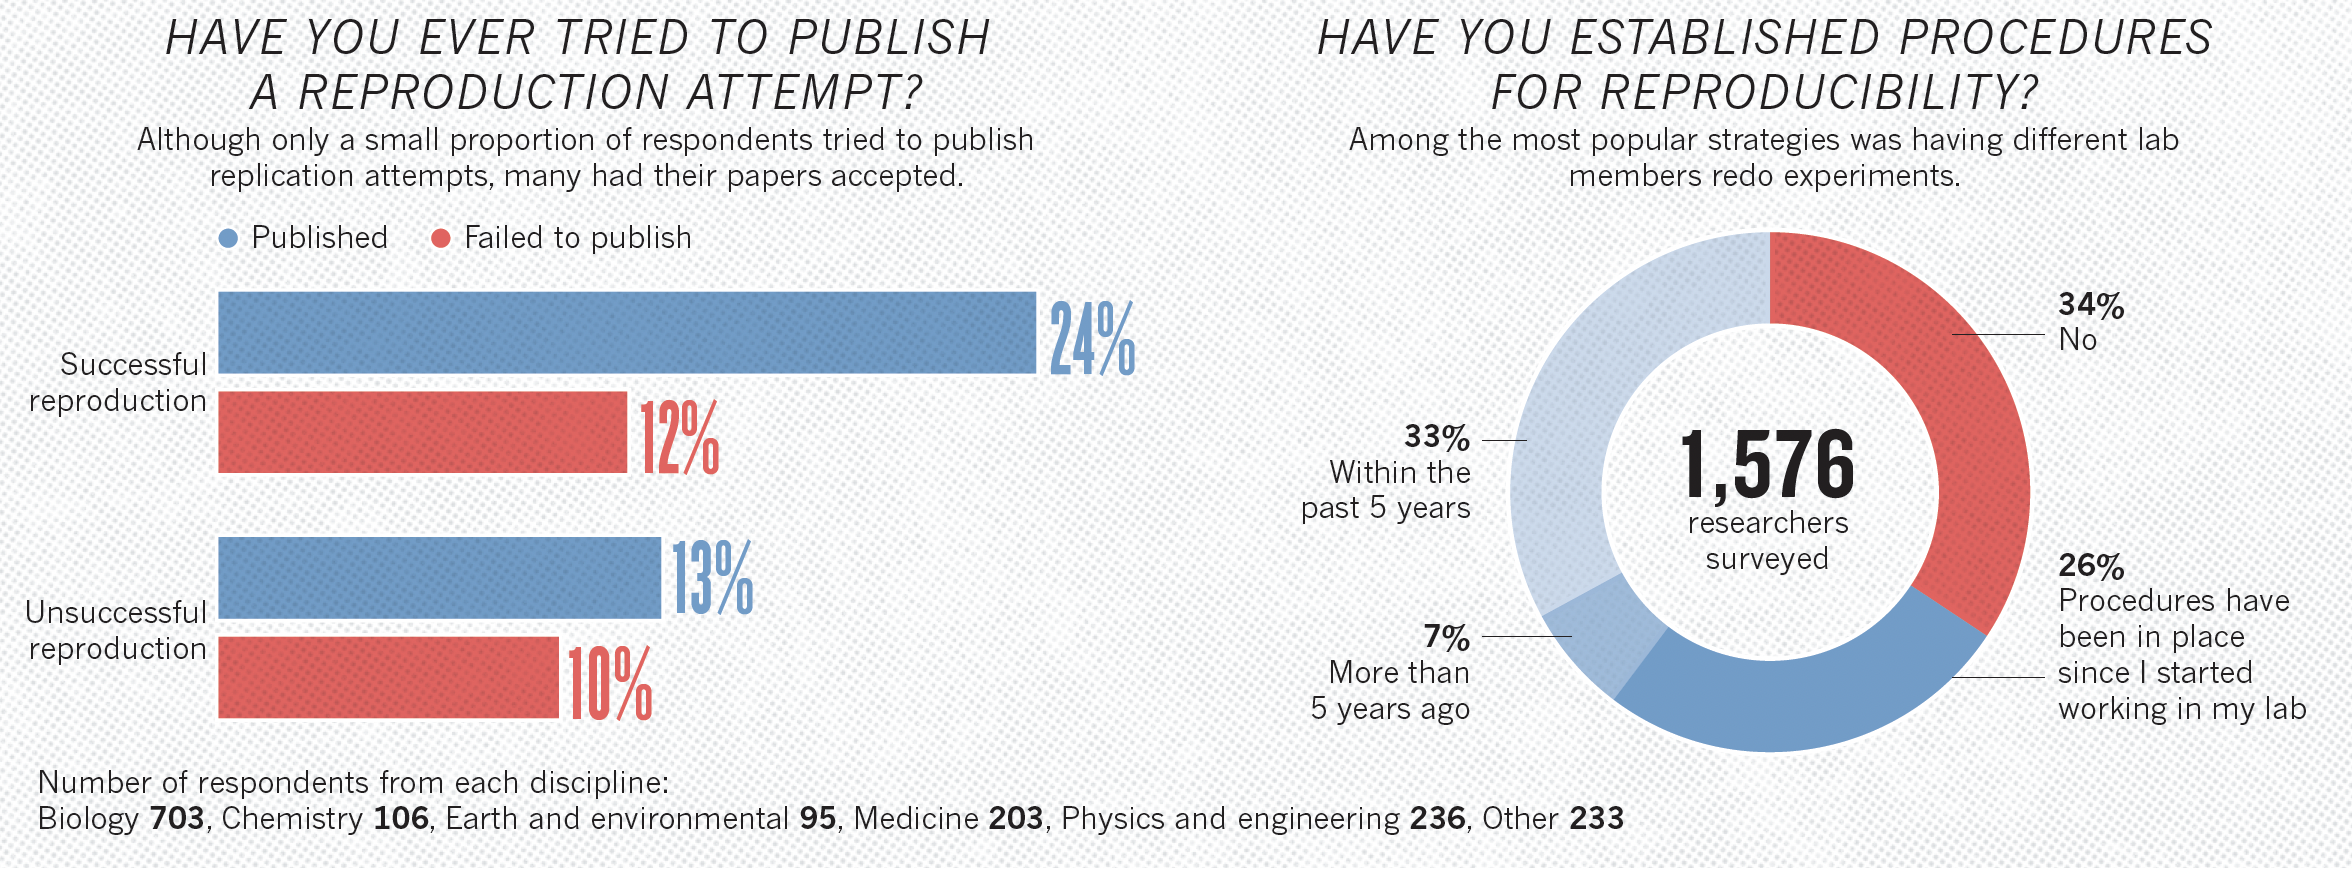
\includegraphics[width=6.5in,height=\textheight]{images/baker-02.png}

Figure 2:Attempts to publish reproducible research (Baker, 2016).

If contributing to science and other researchers seems not to be
compelling enough, here are 5 selfish reasons to work reproducibly
according to Markowetz (2015):

\begin{itemize}
\item
  Helps to avoid data loss and disaster
\item
  Makes it easier to write papers
\item
  Helps reviewers see it your way
\item
  Enables continuity of your work
\item
  Helps to build your reputation
\end{itemize}

\hypertarget{using-rstudio-for-your-project}{%
\section{Using RStudio for your
project}\label{using-rstudio-for-your-project}}

RStudio is an integrated development environment (IDE) for R and Python.
It includes a console, syntax-highlighting editor that supports direct
code execution, as well as tools for plotting, history, debugging,
collaboration, and workspace management. It is a powerful tool which
supports research by weaving the principles of reproducibility
throughout the entire research lifecycle, from data gathering to the
statistical analysis, presentation and publication of results.

\hypertarget{advantages-of-using-rstudio}{%
\subsection{Advantages of Using
RStudio}\label{advantages-of-using-rstudio}}

\begin{itemize}
\tightlist
\item
  It is free and open-source
\item
  It is designed to make it easy to write and reuse code
\item
  Makes it convenient to view and interact with the objects stored in
  your environment
\item
  Makes it easy to set your working directory and access files on your
  computer
\item
  Integrates with Collaboration and Publishing Tools
\item
  Creates documents using R Markdown
\end{itemize}

\hypertarget{setting-up-r-for-projects}{%
\subsection{Setting up R for Projects}\label{setting-up-r-for-projects}}

There are a number of RStudio settings that are recommended. These
settings will force RStudio to start ``fresh'' each time you open
RStudio.

This means that RStudio will not remember the code that you ran in your
previous session. This forces you to document your work in your code and
not in the RStudio workspace {[}which is temporary{]}.

Figure 3 list the preferred RStudio settings. To change these options go
to \textbf{Tools\textgreater Global Options\textgreater General.}

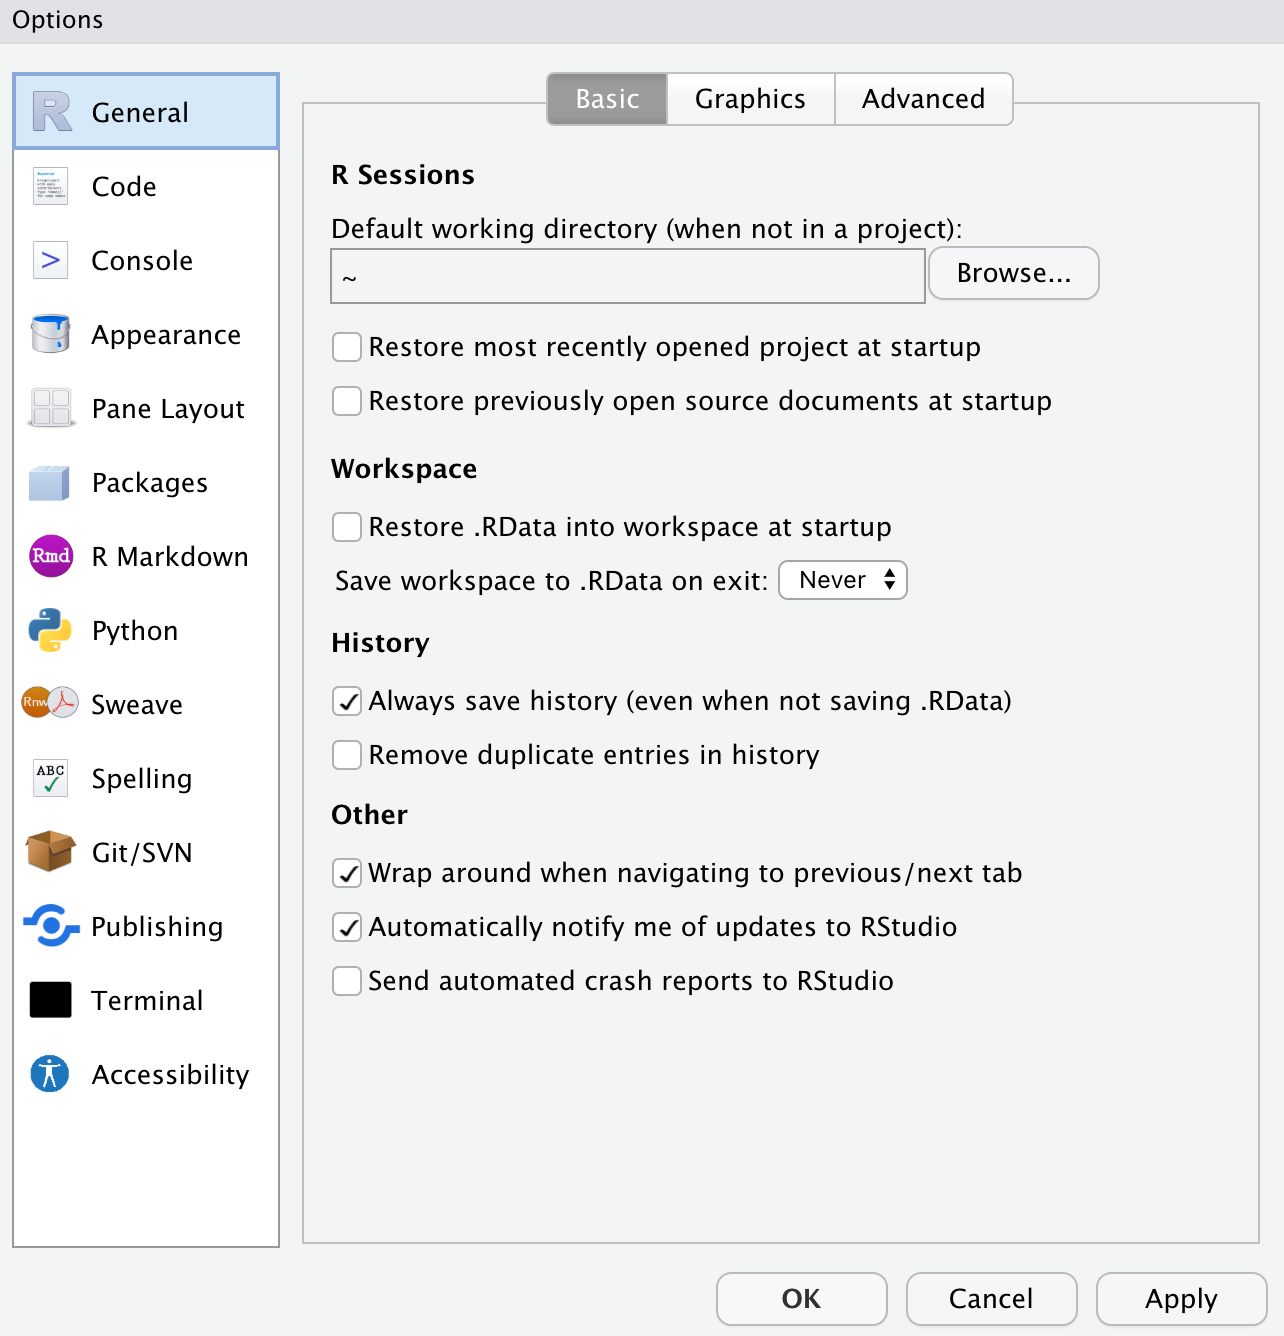
\includegraphics[width=4.5in,height=\textheight]{images/rstudio-preferences.png}

Figure 3: Preferred RStudio options.

You might want to also choose UTF-8 as the default text encoding. This
setting is available from \textbf{Tools\textgreater Global
Options\textgreater Code\textgreater Saving}.

\hypertarget{rstudio-projects}{%
\subsection{RStudio Projects}\label{rstudio-projects}}

An
\href{https://support.rstudio.com/hc/en-us/articles/200526207-Using-Projects}{RStudio
Project} provides a set of tools that allow you to organize your
scripts, files, and output: * Allows you to navigate quickly to your
working directory, and it is a great way to keep all your data
organized. * Can preserve custom settings and open files to make it
easier to resume work after a break. * An RStudio project is different
from an R session. Meaning that an R session is all the objects and work
done in R. Sessions are usually kept in working memory, until you
restart R.

\hypertarget{section}{%
\subsection{}\label{section}}

\hypertarget{creating-a-project-using-version-control-in-rstudio}{%
\section{Creating a Project Using Version Control in
RStudio}\label{creating-a-project-using-version-control-in-rstudio}}

Using version control is a powerful feature to make your research more
reproducible and better organized. In order to use versioning while
working in RStudio the first step is to make sure your work is set up as
an R Project, because you may not use the versioning features in RStudio
without one. There are three options for doing this depending on your
given scenario:

\begin{enumerate}
\def\labelenumi{\arabic{enumi}.}
\tightlist
\item
  New Directory - start a brand new R project (with the option of
  version control).
\item
  Existing Directory - add existing work to a R project (with the option
  of setting up version control).
\item
  Version Control Continue an existing R project that already uses
  version control (i.e.~download from GitHub).
\end{enumerate}

We will be using option 3, setting an R project on GitHub and then
importing this into RStudio.

\#\#About Authentication to GitHub

You can securely access your account's resources by authenticating to
GitHub, using different credentials depending on where you authenticate.

To keep your account secure, you must authenticate before you can access
certain resources on GitHub. When you authenticate to GitHub, you supply
or confirm credentials that are unique to you to prove that you are
exactly who you declare to be.

You can access your resources in GitHub in a variety of ways: in the
browser, via GitHub Desktop or another desktop application, with the
API, or via the command line. Each way of accessing GitHub supports
different modes of authentication.

\begin{itemize}
\item
  Username and password with two-factor authentication
\item
  Personal access token
\item
  SSH key
\end{itemize}

\#\#Authenticating in your browser**

You will authenticate using your GitHub.com username and password. You
may also use two-factor authentication and SAML single sign-on, which
can be required by organization and enterprise owners. The help
\href{https://docs.github.com/en/authentication/keeping-your-account-and-data-secure/about-authentication-to-github}{documentation}
for this topic on GitHub is an excellent resource. I will talk about
sync issues in a separate section.

\#\#Choosing a URL for your remote repository**

There are several ways to clone repositories available on GitHub.com.

When you view a repository while signed in to your account, the URLs you
can use to clone the project onto your computer are available below the
repository details.

For information on setting or changing your remote URL, see
``\href{https://docs.github.com/en/github/getting-started-with-github/managing-remote-repositories}{Managing
remote repositories}.''

\hypertarget{creating-a-new-repository-in-github}{%
\subsection{Creating a New Repository in
GitHub}\label{creating-a-new-repository-in-github}}

GitHub's collaborative approach to development depends on publishing
commits from your local repository to GitHub for other people to view,
fetch, and update.

\href{https://github.com/signup}{At this link}, you may sign into your
GitHub account or create one if you have not already.

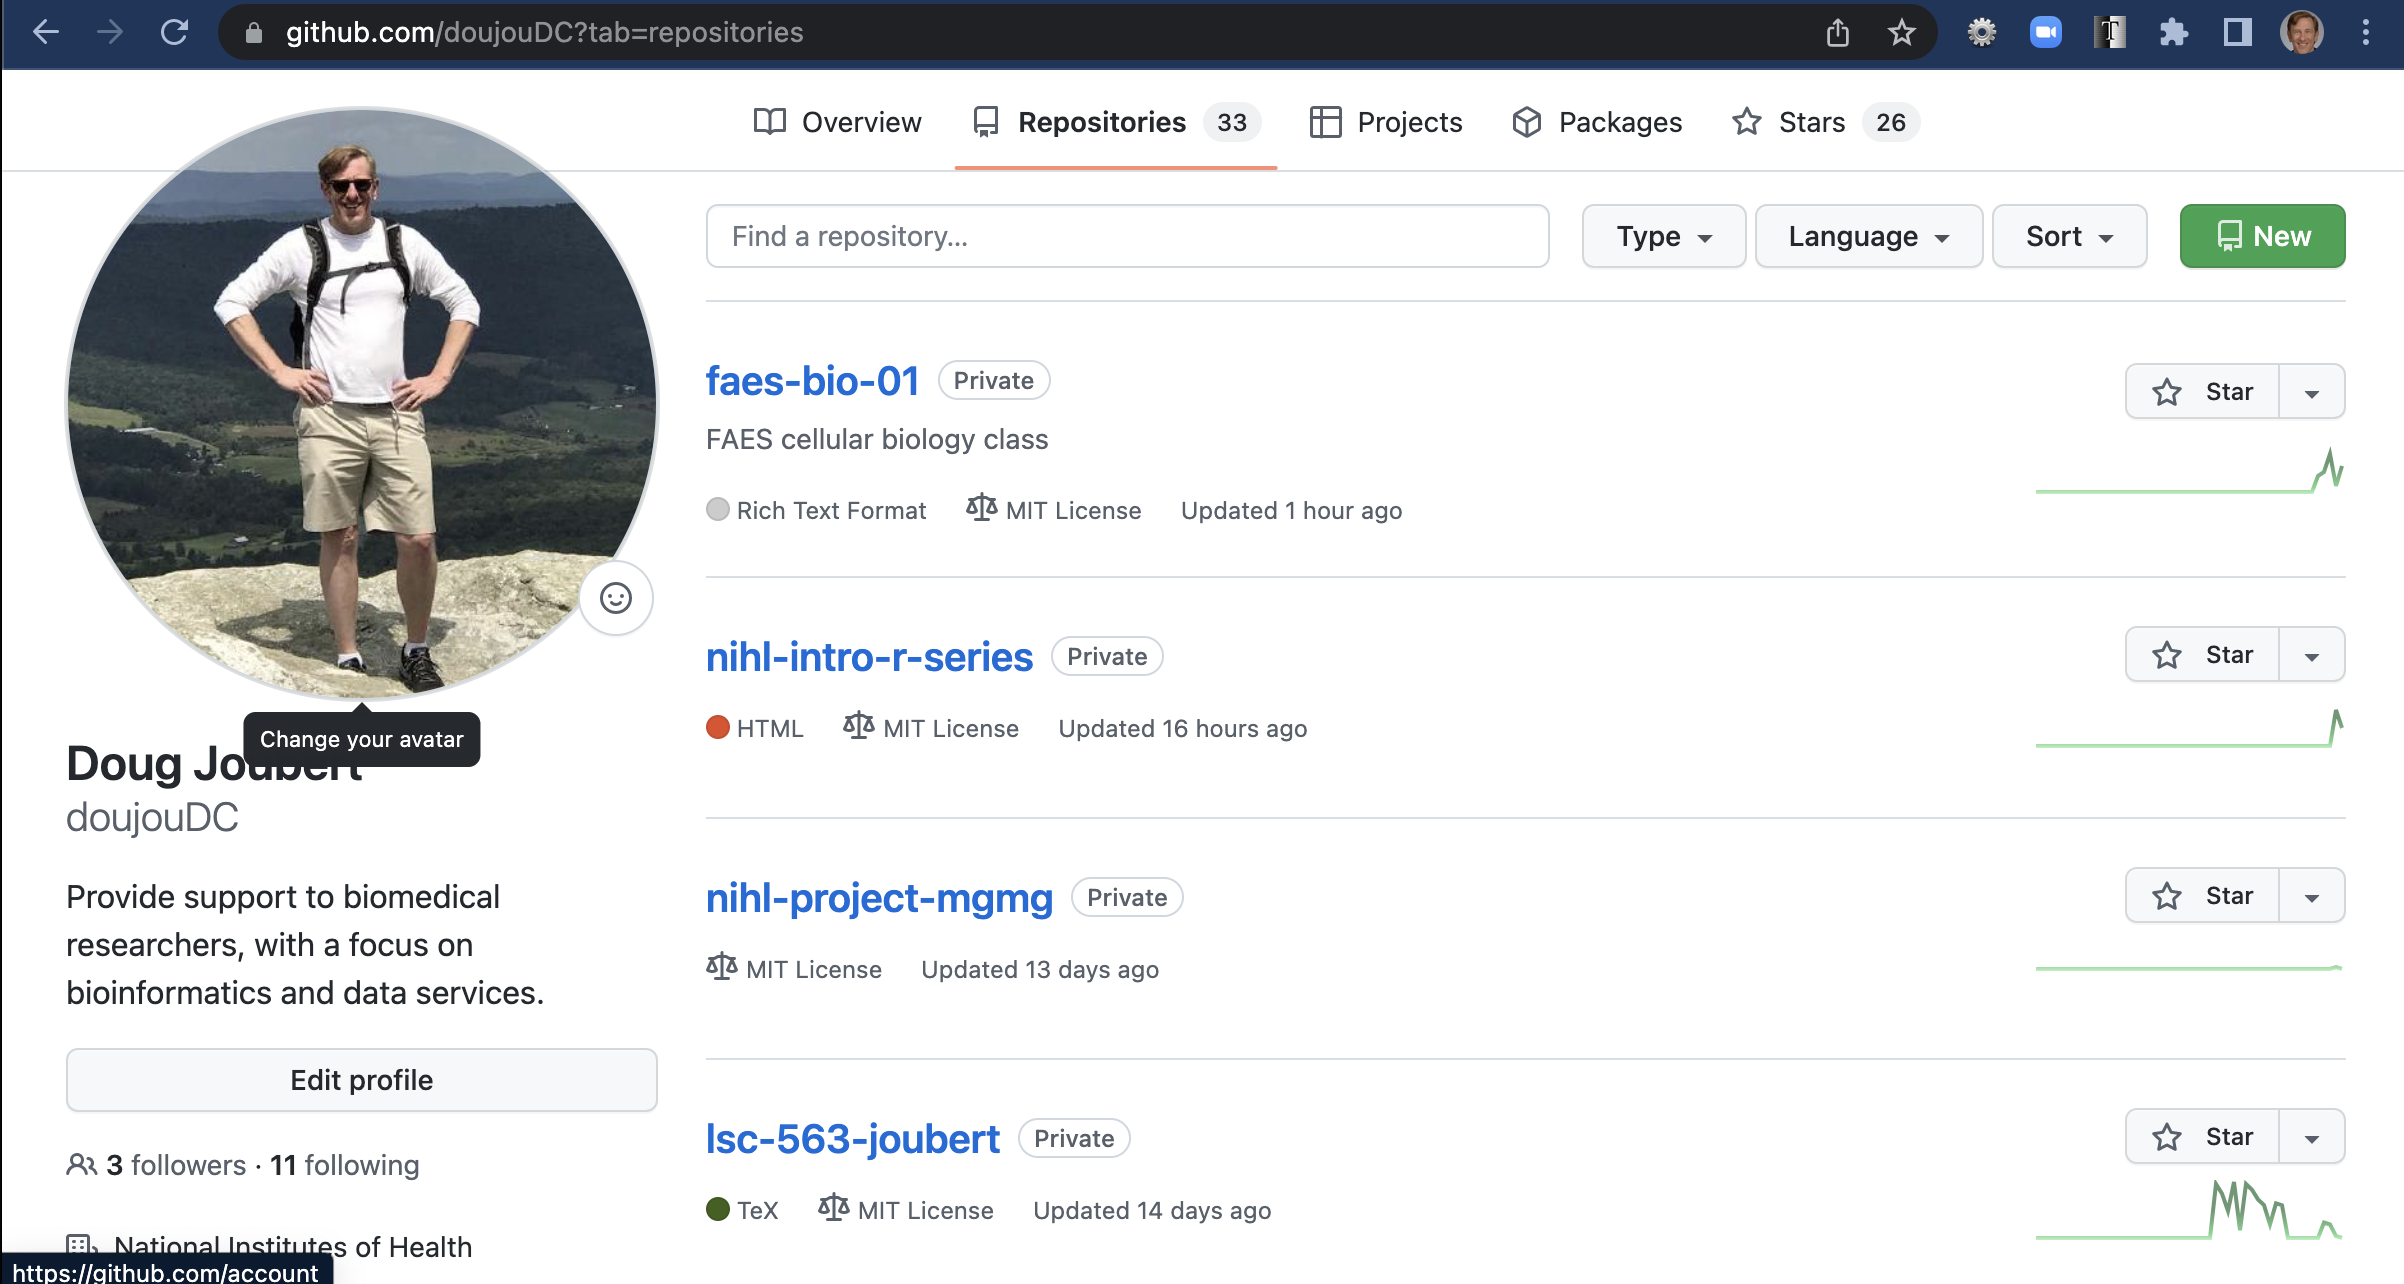
\includegraphics[width=6.5in,height=\textheight]{images/git-hub-01.png}

Figure 4: My repository homepage in GitHub

I have already created a
\href{https://github.com/doujouDC/nihl-intro-r-series.git}{repository}
for this class. However Figure 5 is displaying the Create a New
Repository screen. {[}Figure 5{]}.

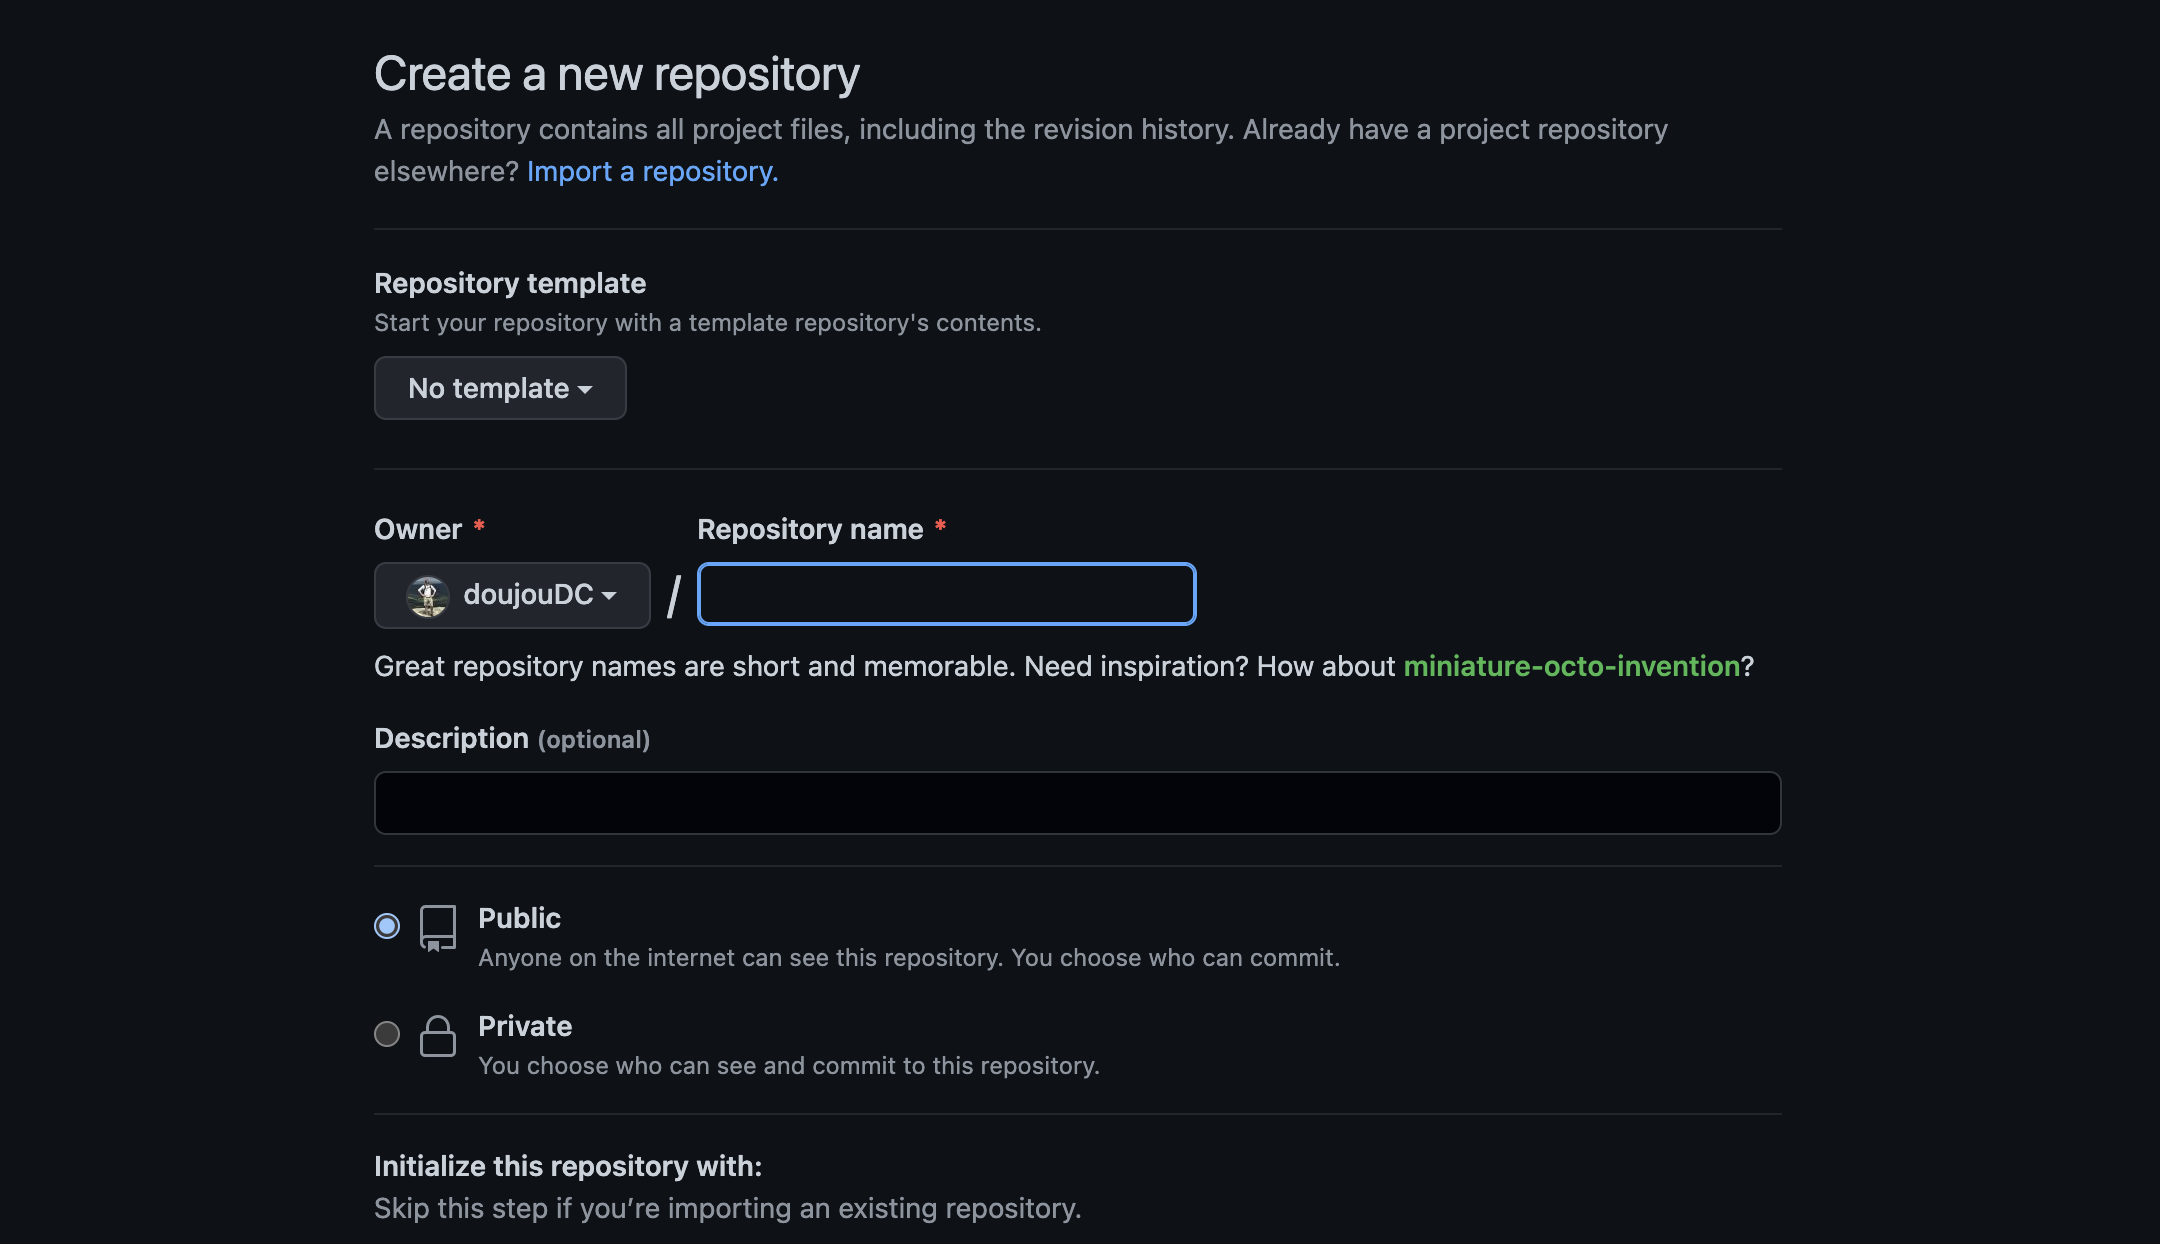
\includegraphics[width=6.5in,height=\textheight]{images/git-hub-02.png}

Figure 5: Creating a new repository on GitHub.

Once your repository is created, you will need to copy the repository
URL before you create the project in RStudio {[}Figure 6{]}. Figure 6
shows the 3 different methods for creating a URL: (1) https, (2) SSH, or
(3) GitHub CLI.

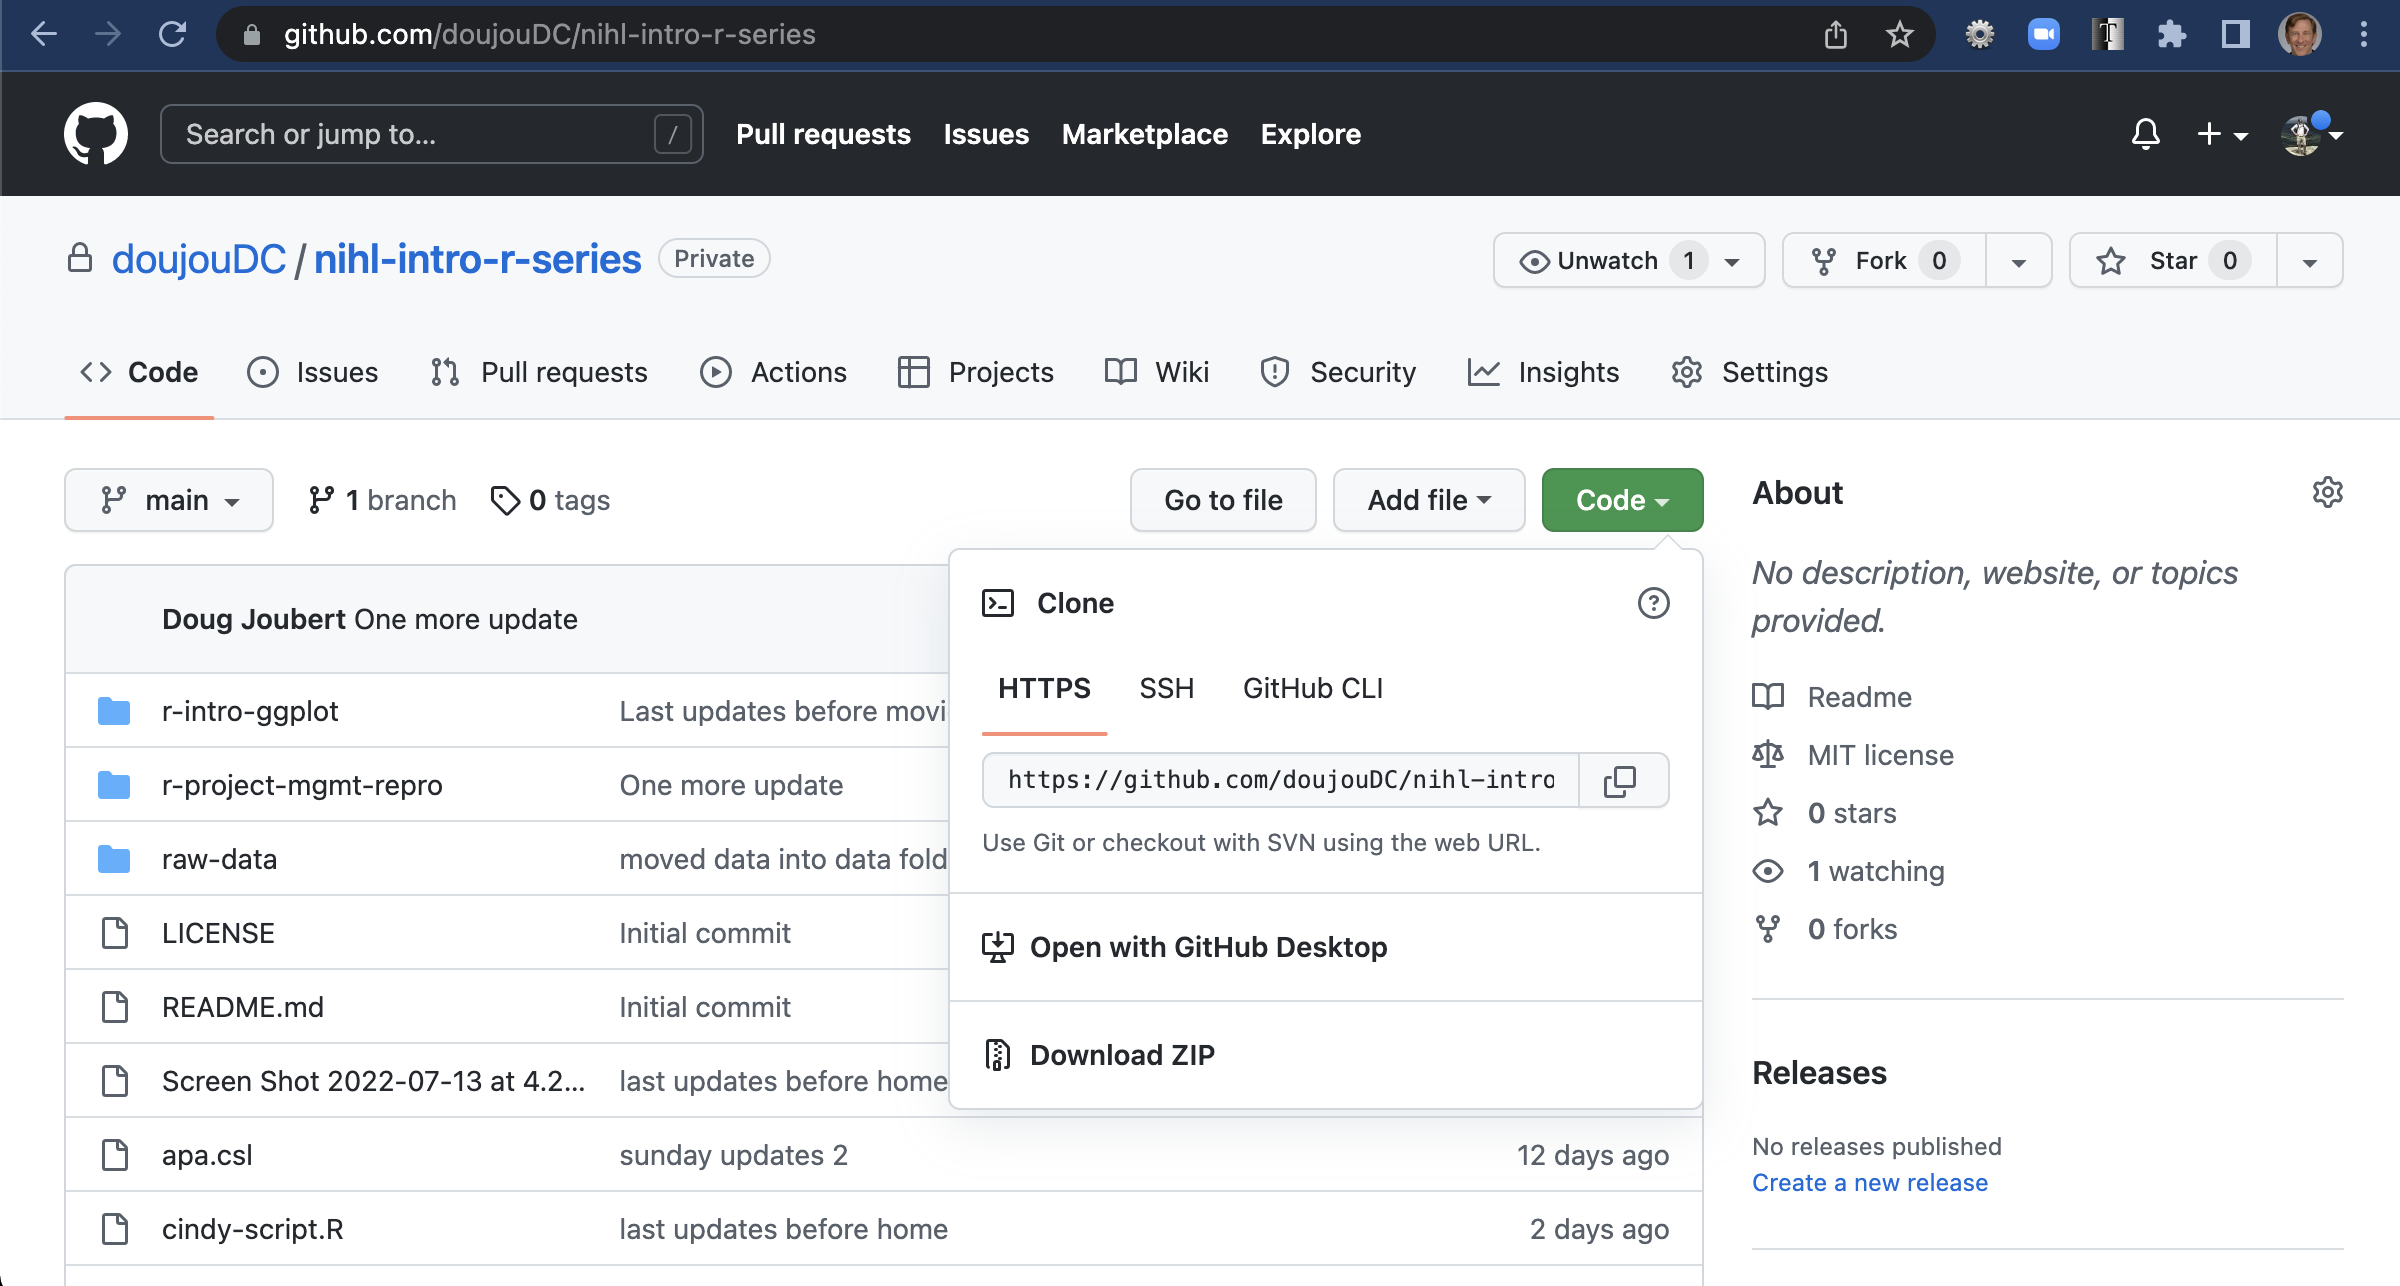
\includegraphics[width=6.5in,height=\textheight]{images/git-hub-03.png}

Figure 6: Creating a link to a GitHub repository.

The ability to create an SSH key is location under settings {[}Figure
7{]}.

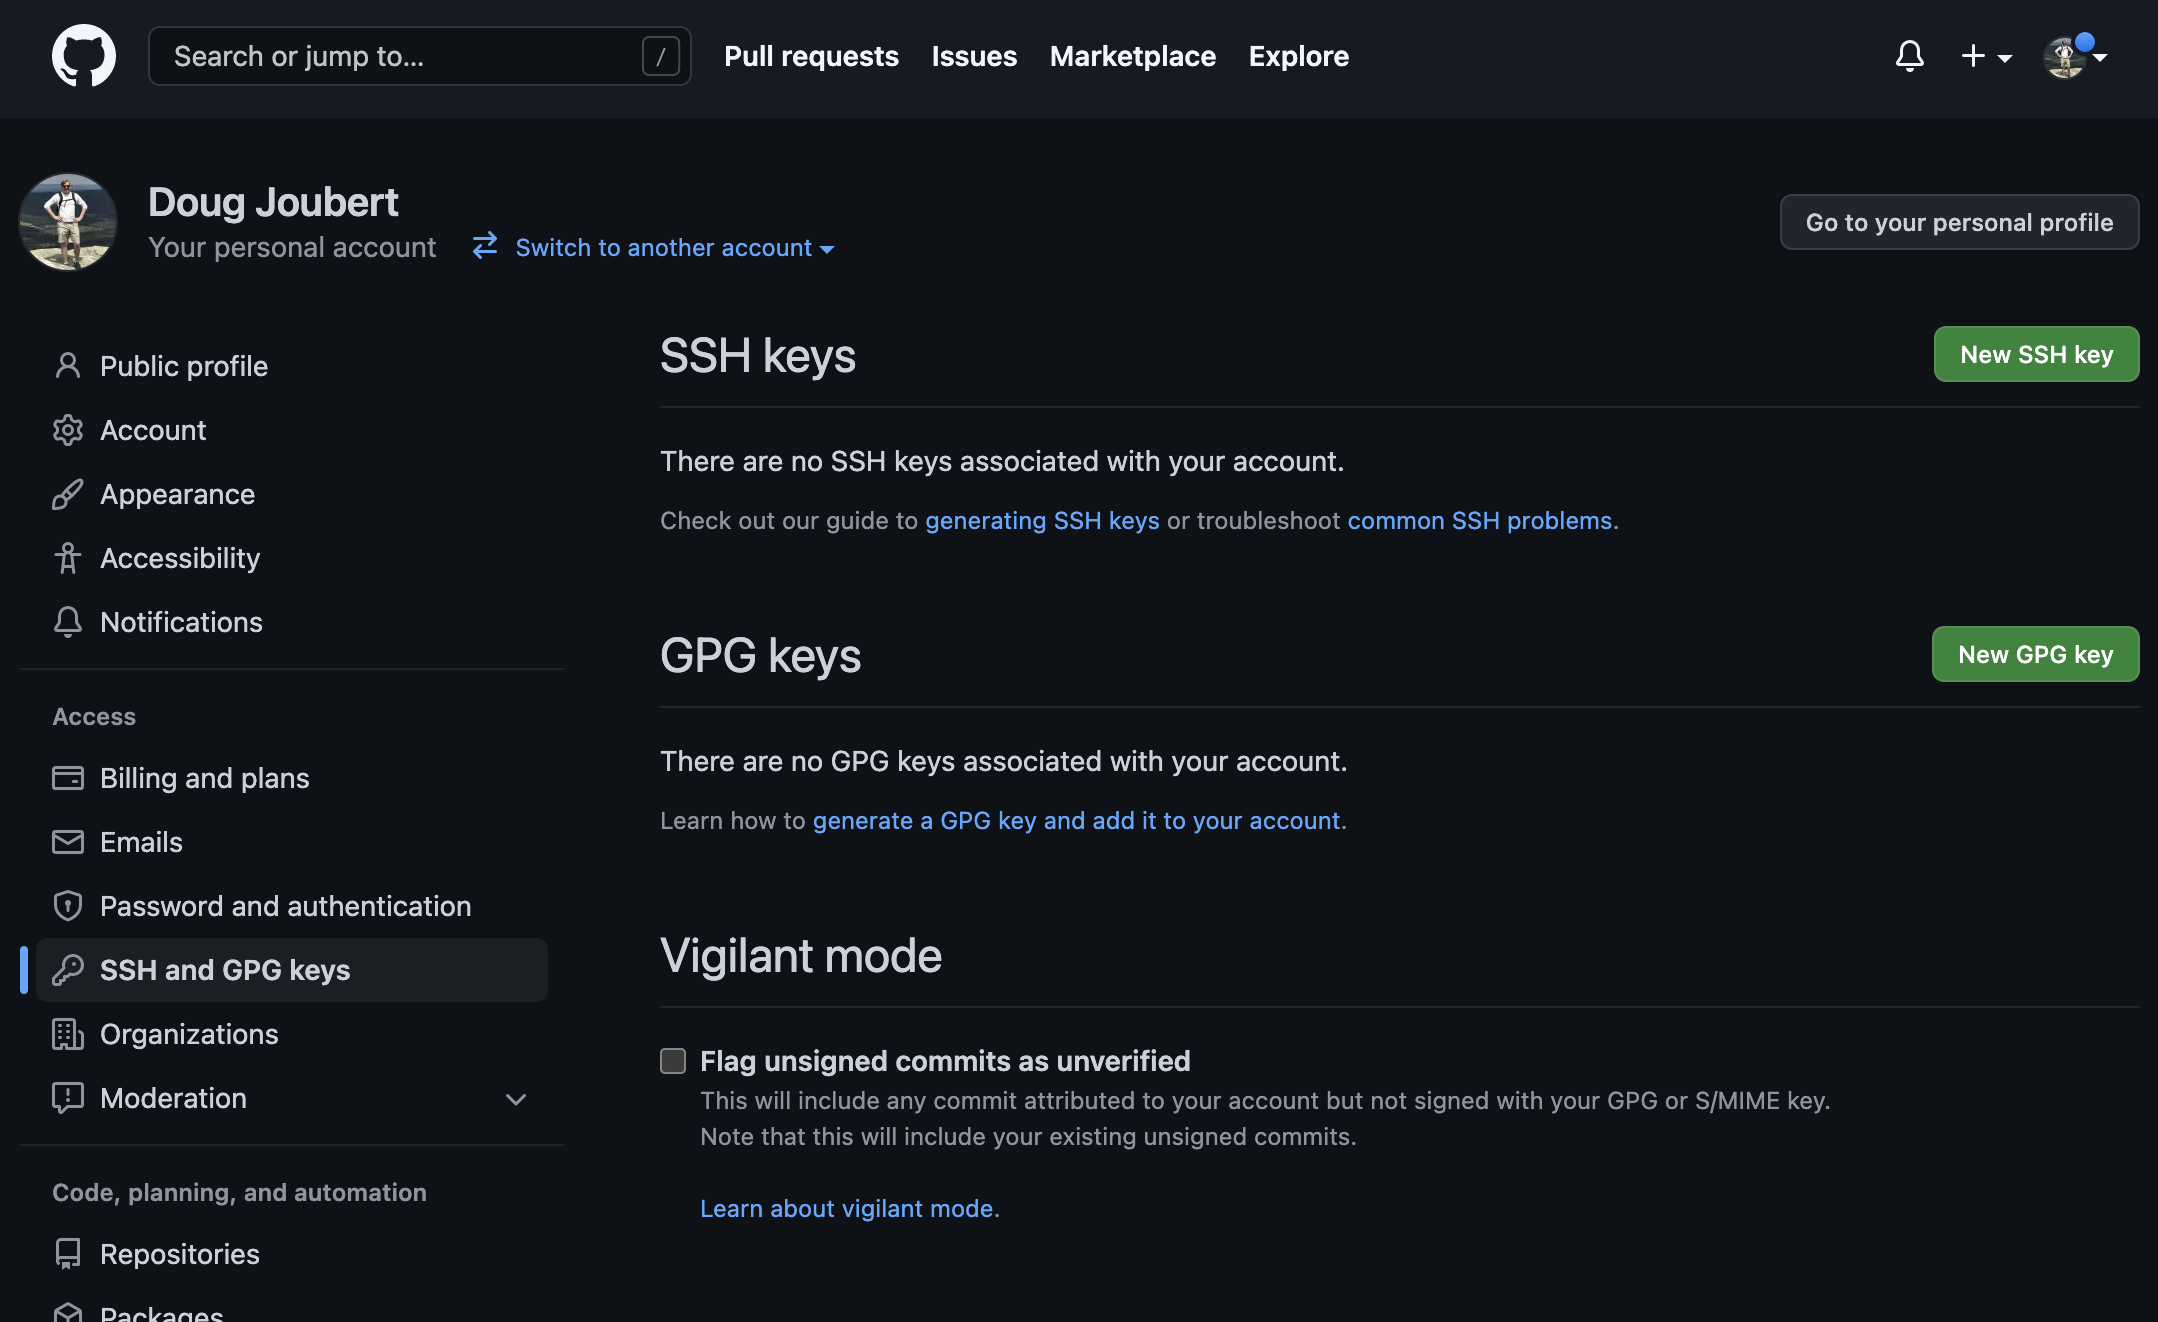
\includegraphics[width=6.5in,height=\textheight]{images/git-hub-05.png}

Figure 7: Creating SSH keys in GitHub.

\hypertarget{before-you-sync-your-repository}{%
\subsection{Before you ``Sync'' Your
Repository}\label{before-you-sync-your-repository}}

Depending on the authentic methods that you have in GitHub, you might
also need to create a Personal Access Token that is used to connect
RStudio to GitHub, the first time you sync {[}Figure 8{]}.

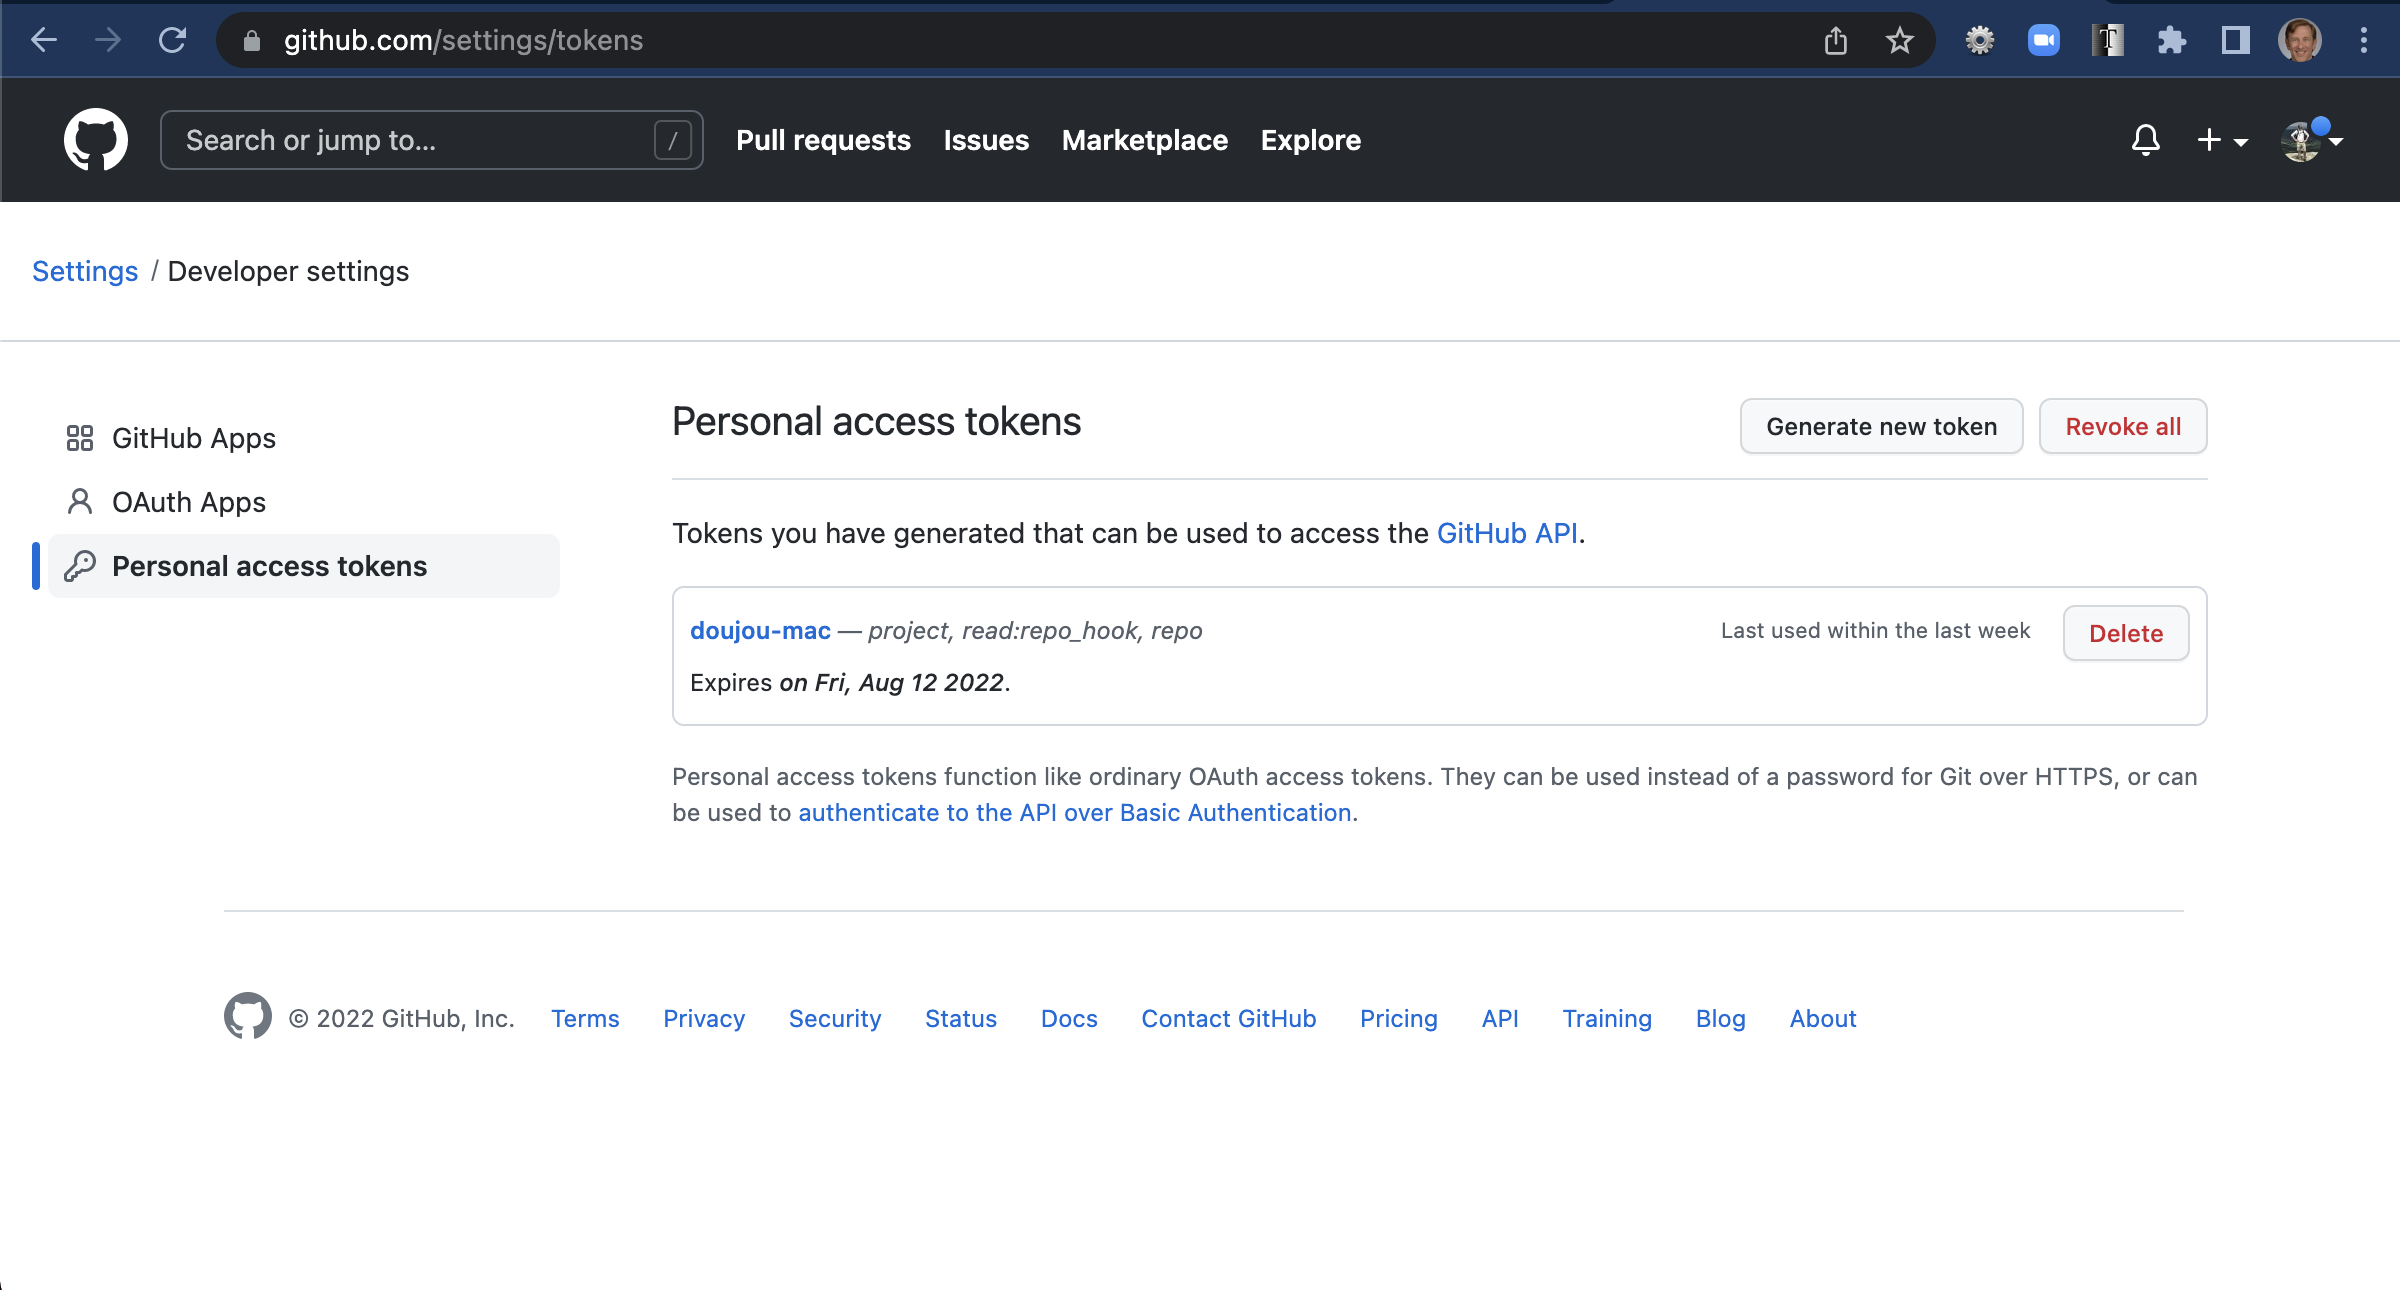
\includegraphics[width=6.5in,height=\textheight]{images/git-hub-04.png}

Figure 8: Creating a Personal Access Code in GitHub.

Depending on the OS that you use, you might need to authenticate via the
RStudio Shell. The RStudio Terminal is accessed from the Tools menu.

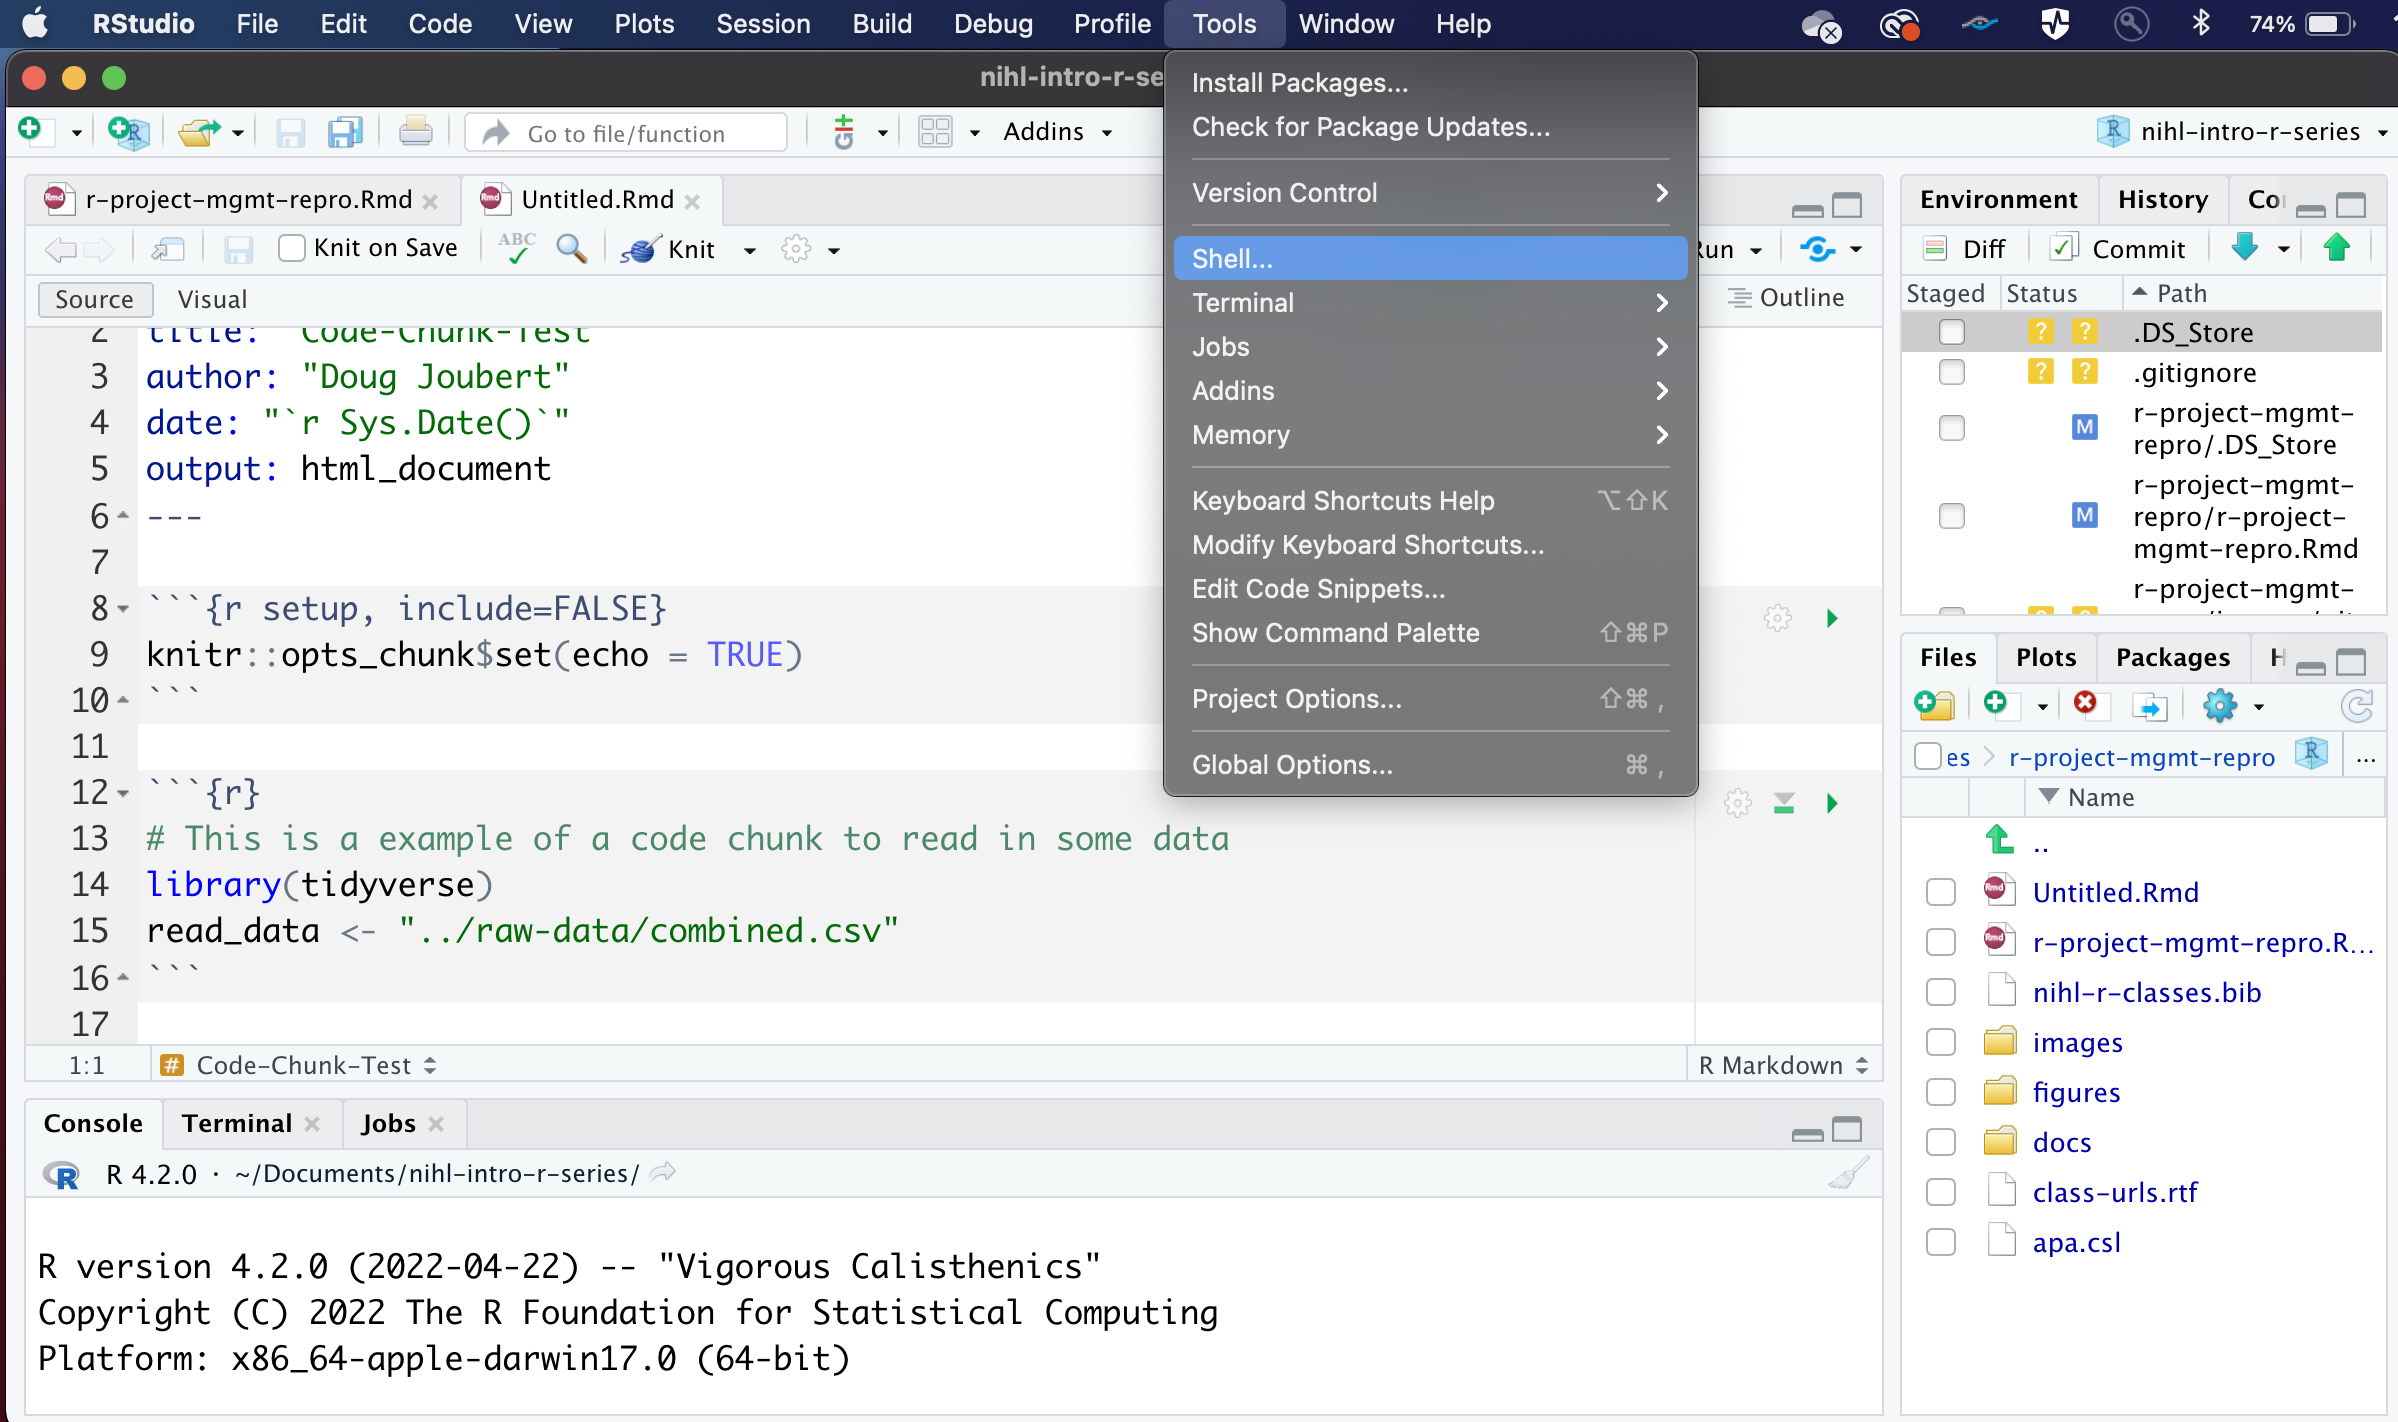
\includegraphics[width=6.5in,height=\textheight]{images/git-hub-06.png}

Figure 9: Connecting to the Shell via RStudio.

The first time to connect to your remote repository, you be prompted to
enter your username and password via the Shell {[}Figure 10{]}.

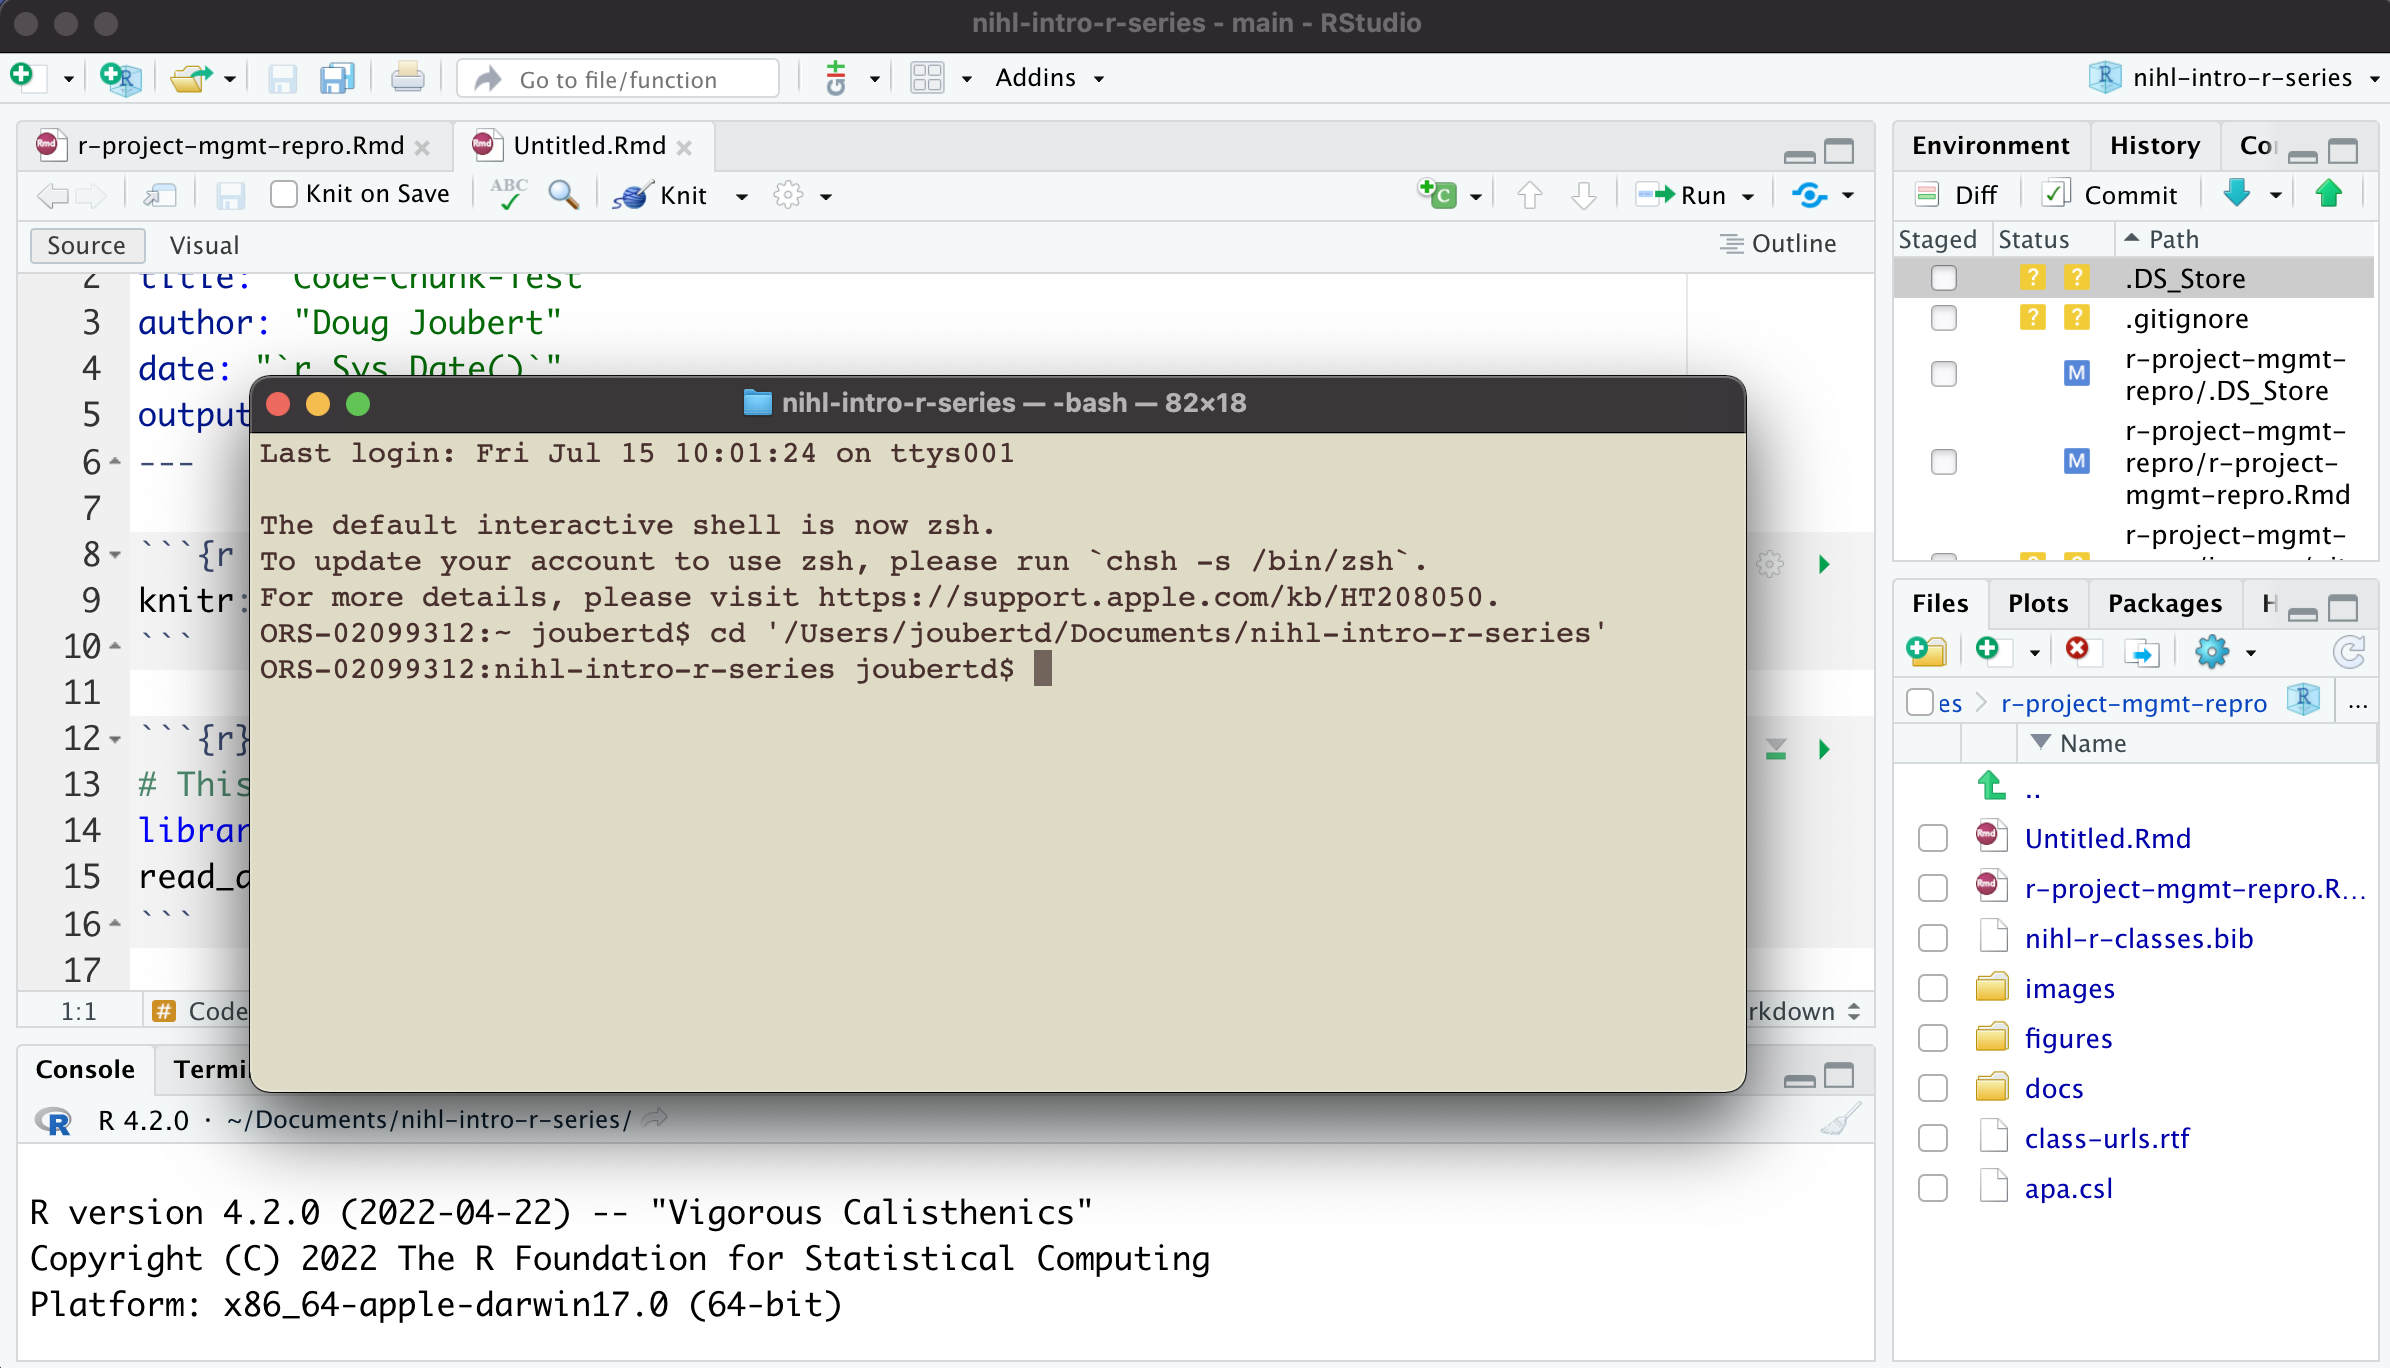
\includegraphics[width=6.5in,height=\textheight]{images/git-01.png}

Figure 10: Accessing a project via the Shell.

As you can see I am in the project working directory:
\texttt{ORS-02099312:nihl-intro-r-series\ joubertd\$}~If I type
\texttt{ls}, I will see all of the files in my working directory
{[}Figure 11{]}. There will be no folders when you first create a new
project.

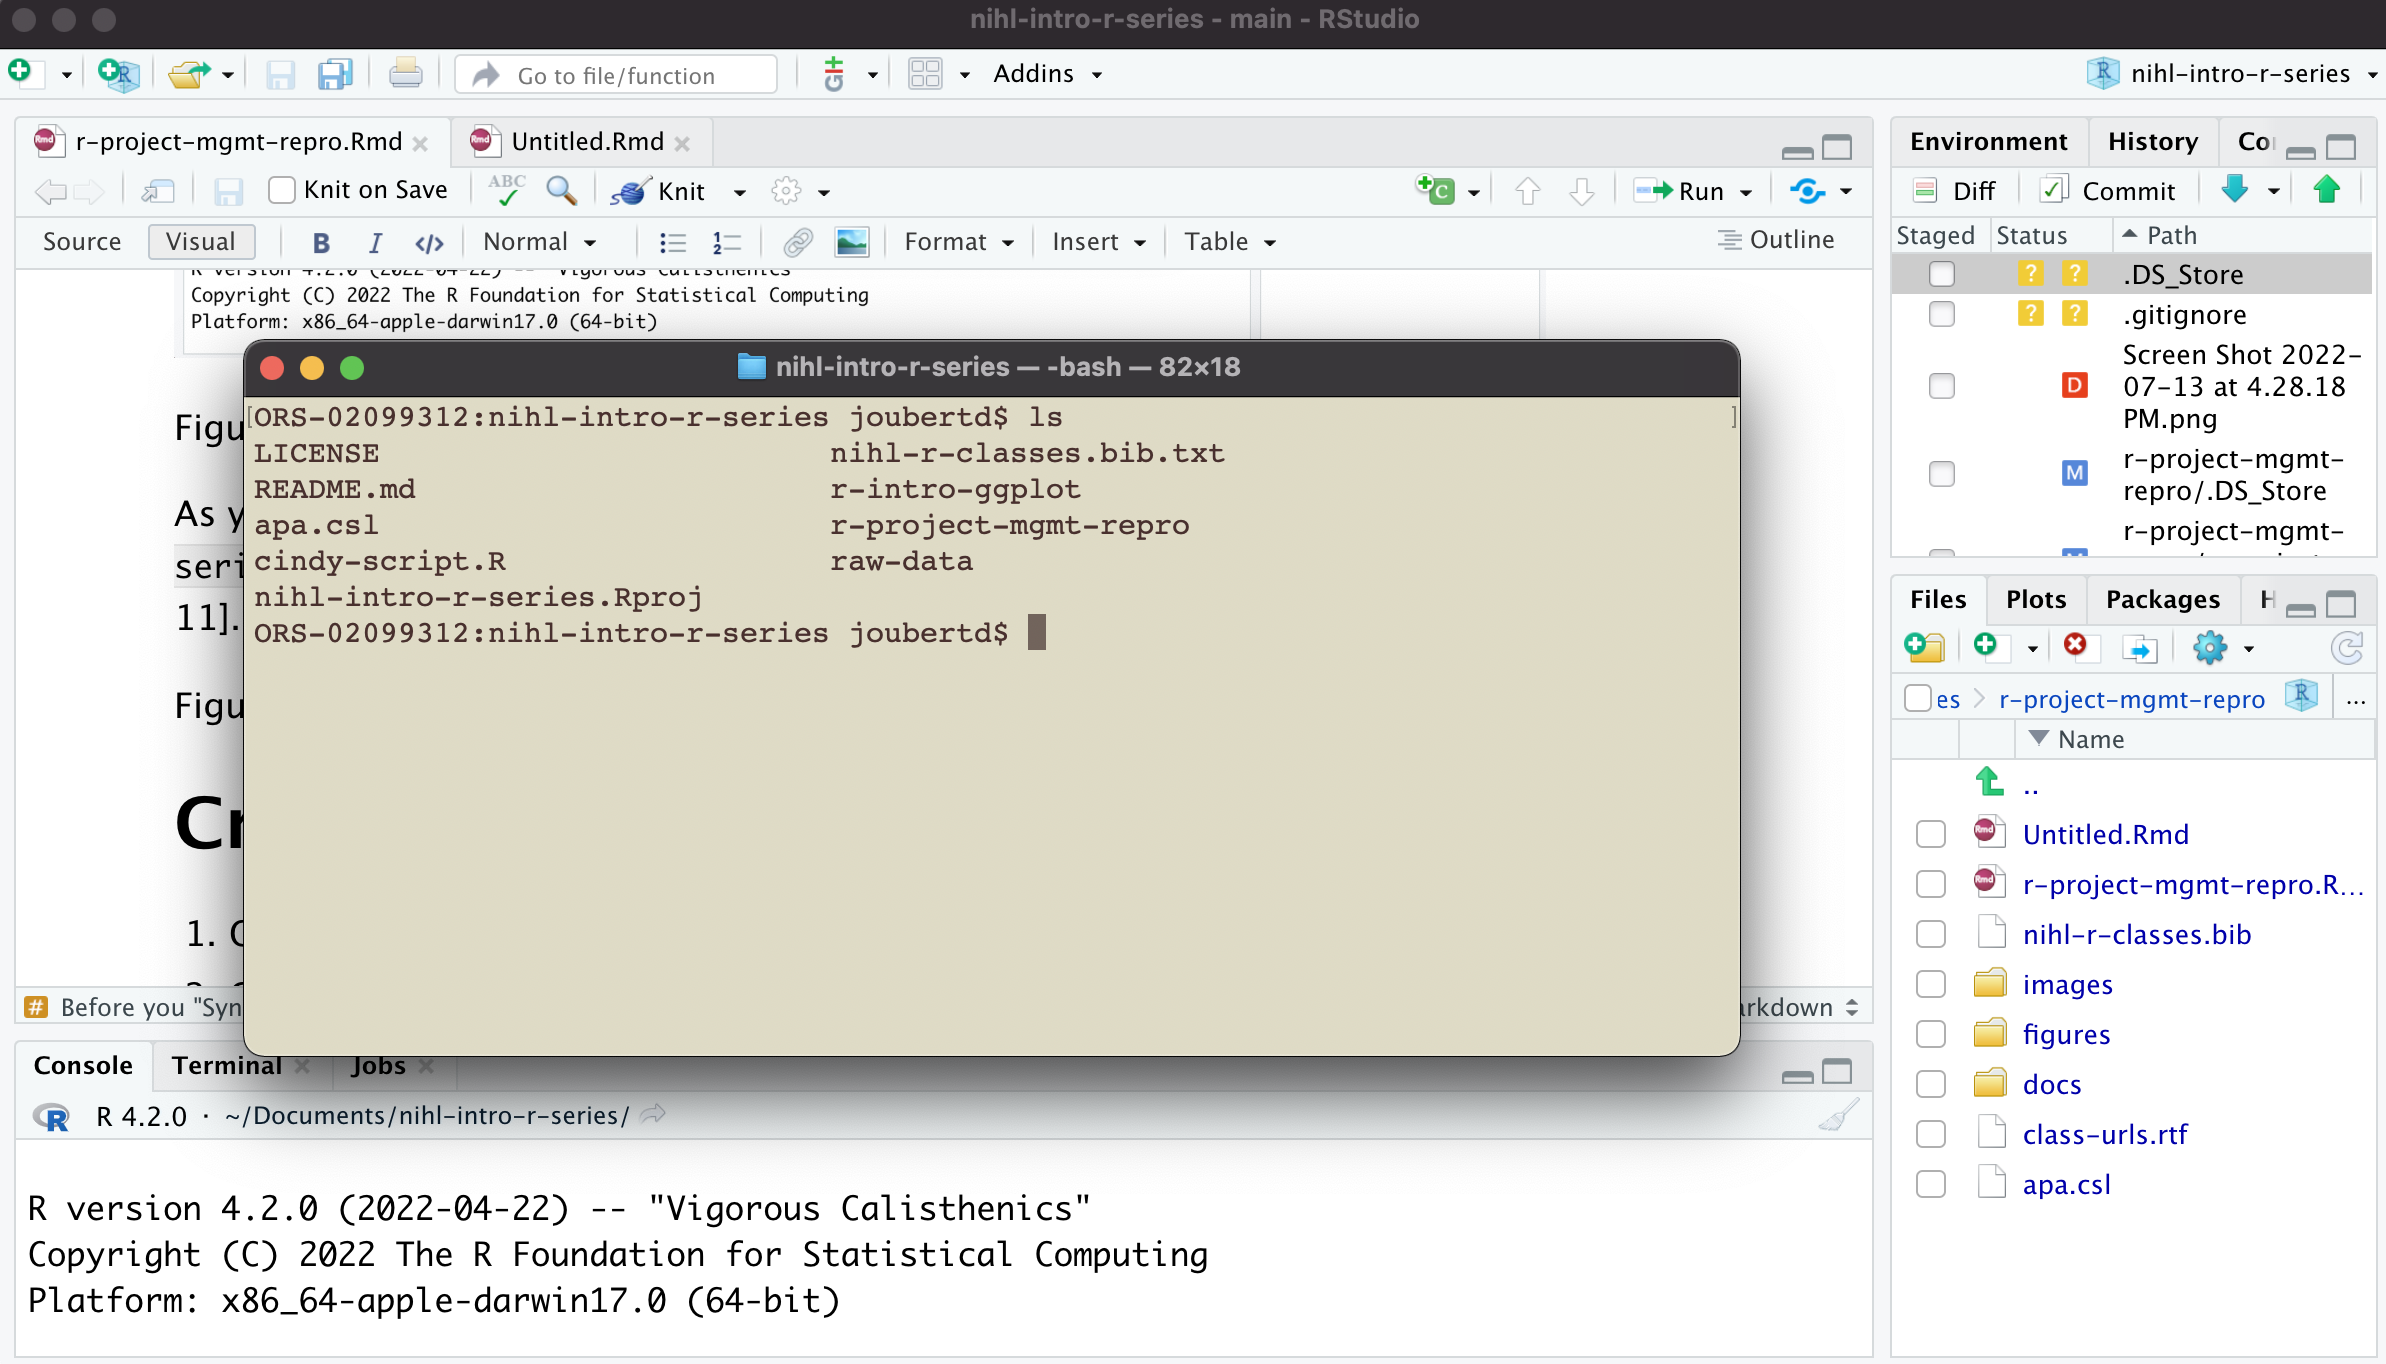
\includegraphics[width=6.5in,height=\textheight]{images/git-02.png}

Figure 11: Files structure in my working directly.

If you need a refresher, the Carpentries have a great
\href{https://swcarpentry.github.io/git-novice/}{lesson} on using GIT.

\hypertarget{creating-a-new-project-in-rstudio}{%
\section{Creating a New Project in
RStudio}\label{creating-a-new-project-in-rstudio}}

\begin{enumerate}
\def\labelenumi{\arabic{enumi}.}
\tightlist
\item
  Open RStudio
\item
  Choose New Project from the Tools Menu.
\item
  There are three options when creating a new project: (1) Creating a
  project in a new directory, (2) Creating a project in an existing
  directory, and (3) Creating a project using version control.
\end{enumerate}

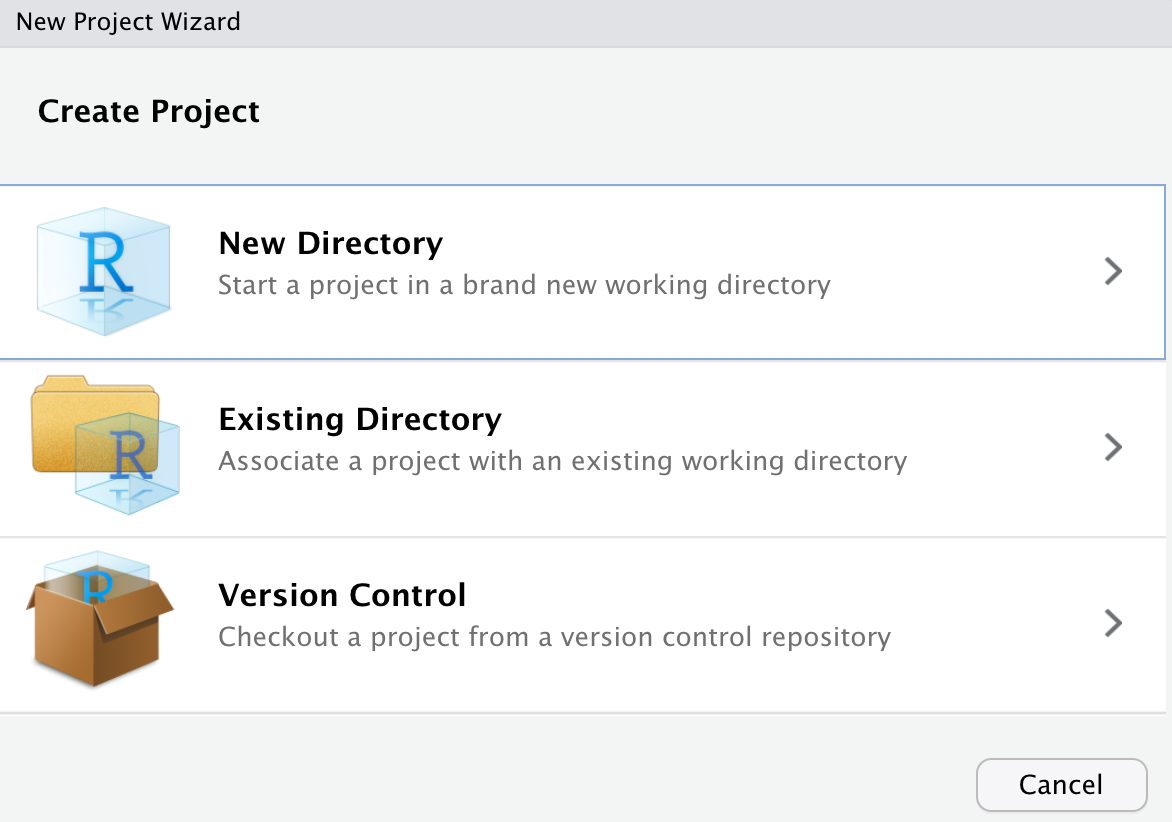
\includegraphics[width=4.5in,height=\textheight]{images/new-project-01.png}

Figure 9: Creating a new project in RStudio.

\begin{enumerate}
\def\labelenumi{\arabic{enumi}.}
\setcounter{enumi}{3}
\tightlist
\item
  Choose the Version Control option
\item
  Chose Git as the option, RStudio will automatically open the next
  screen
\end{enumerate}

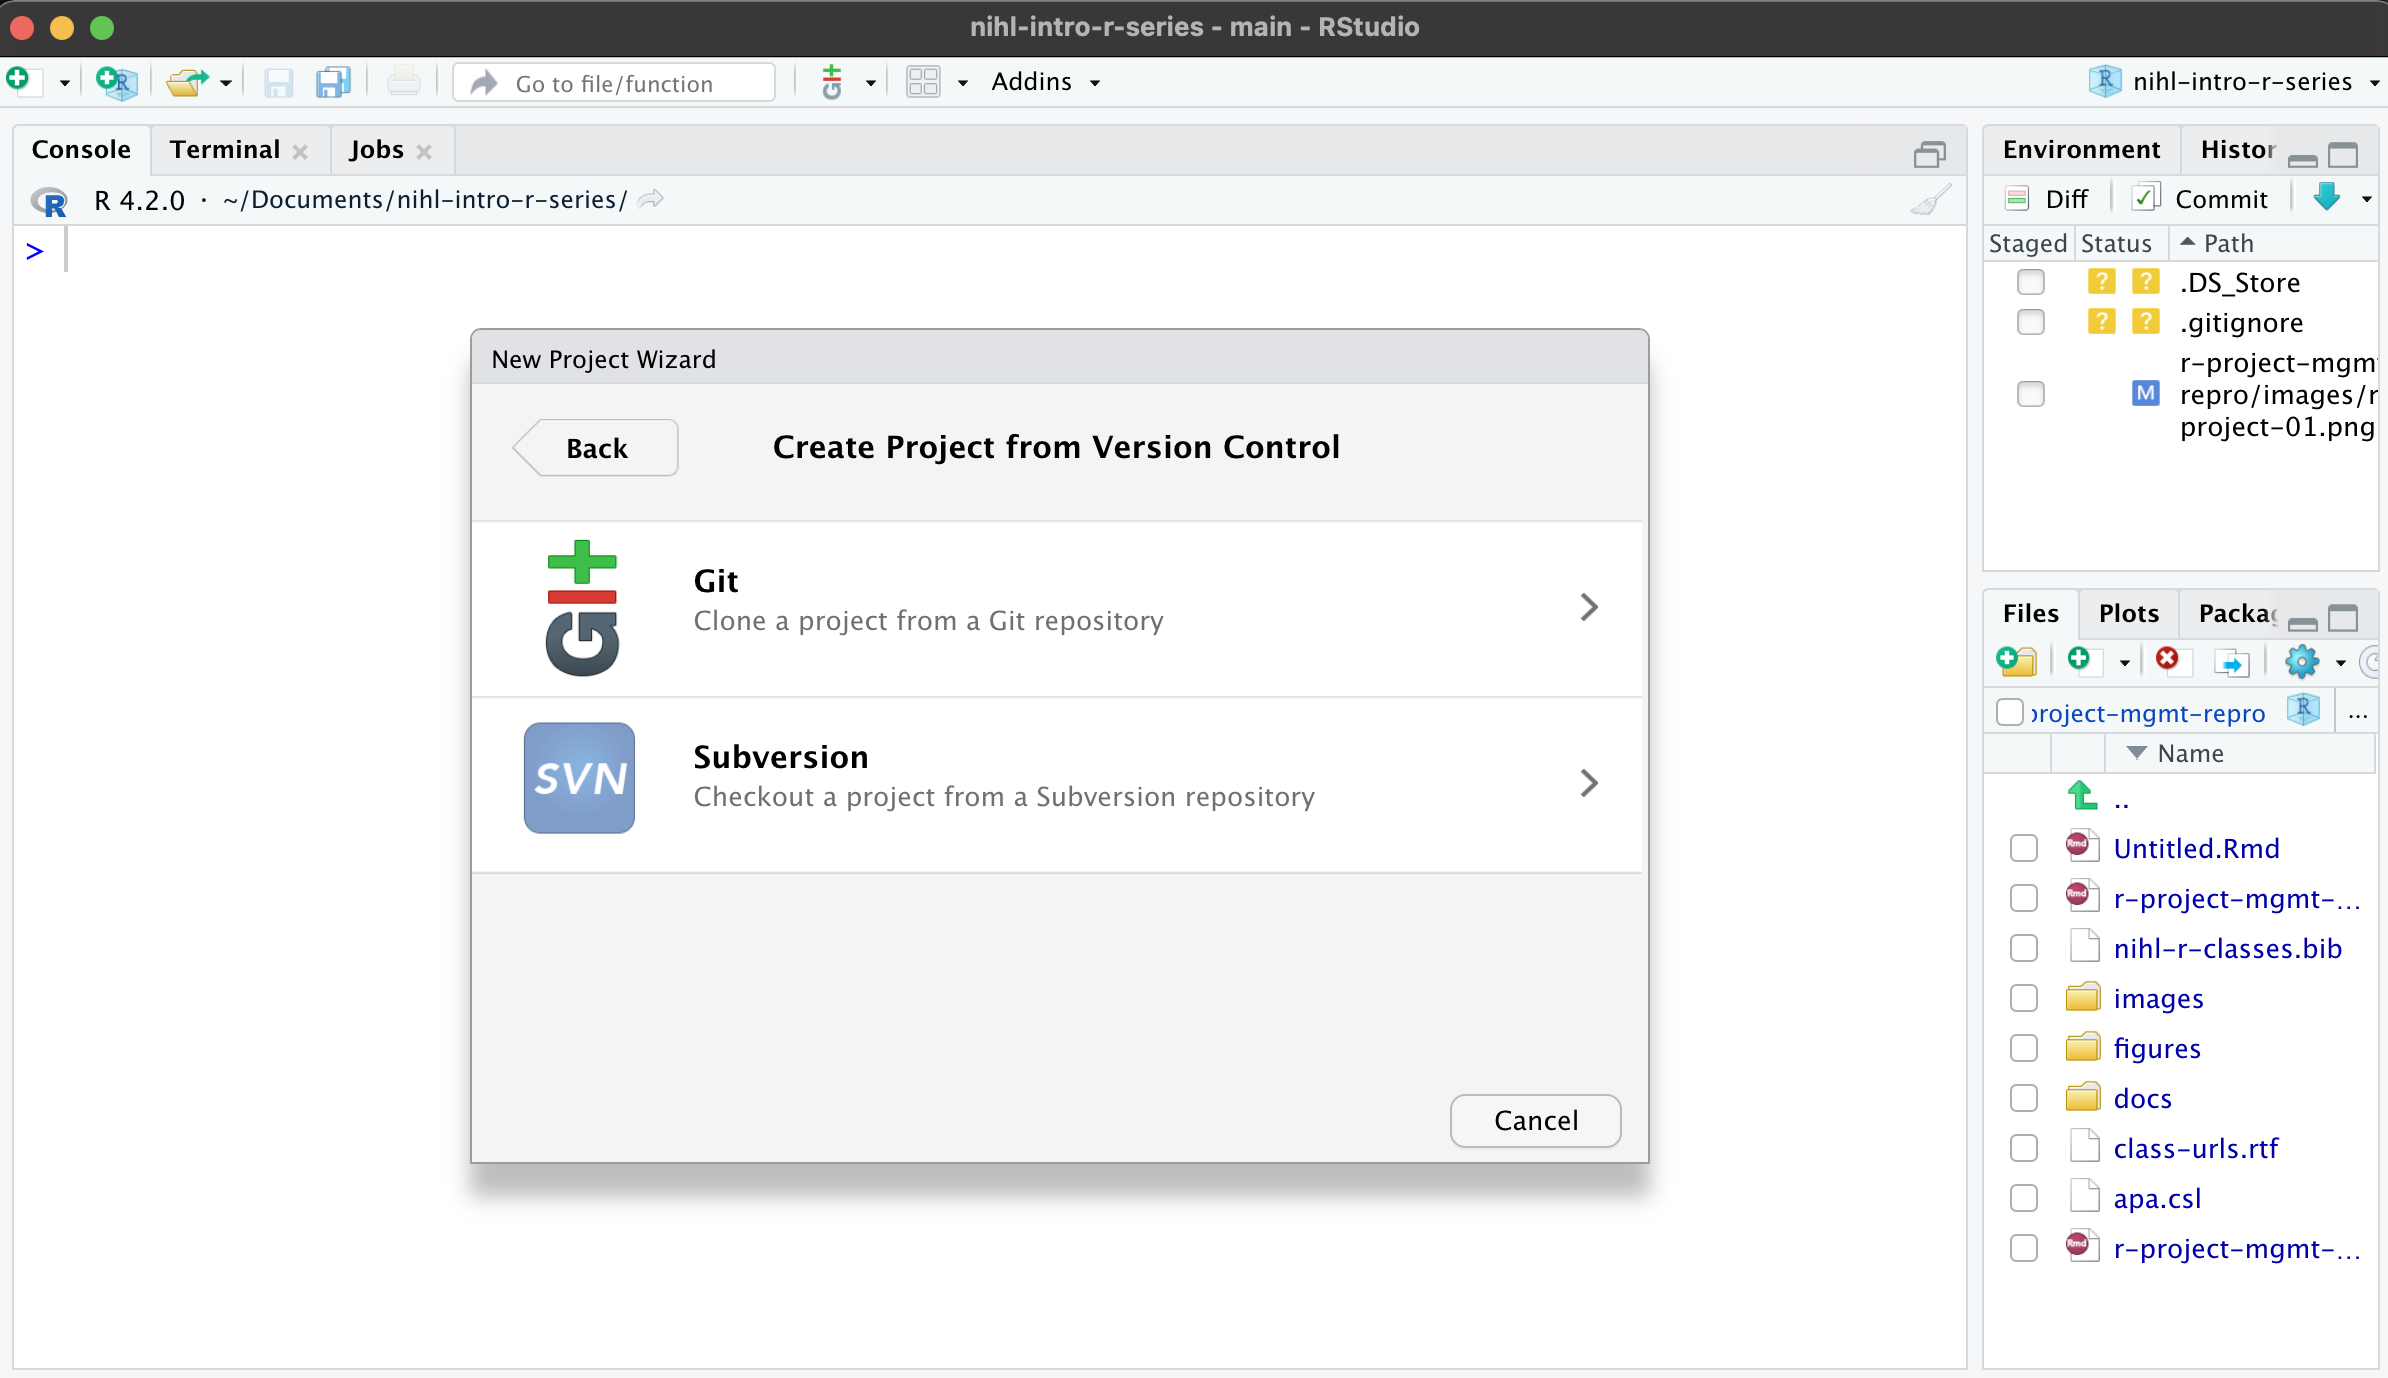
\includegraphics[width=4.5in,height=\textheight]{images/new-project-02.png}

Figure 10: Choosing the version control option in RStudio.

\begin{enumerate}
\def\labelenumi{\arabic{enumi}.}
\setcounter{enumi}{5}
\tightlist
\item
  This screen is where you enter the repository URL that you copied from
  GitHub
\end{enumerate}

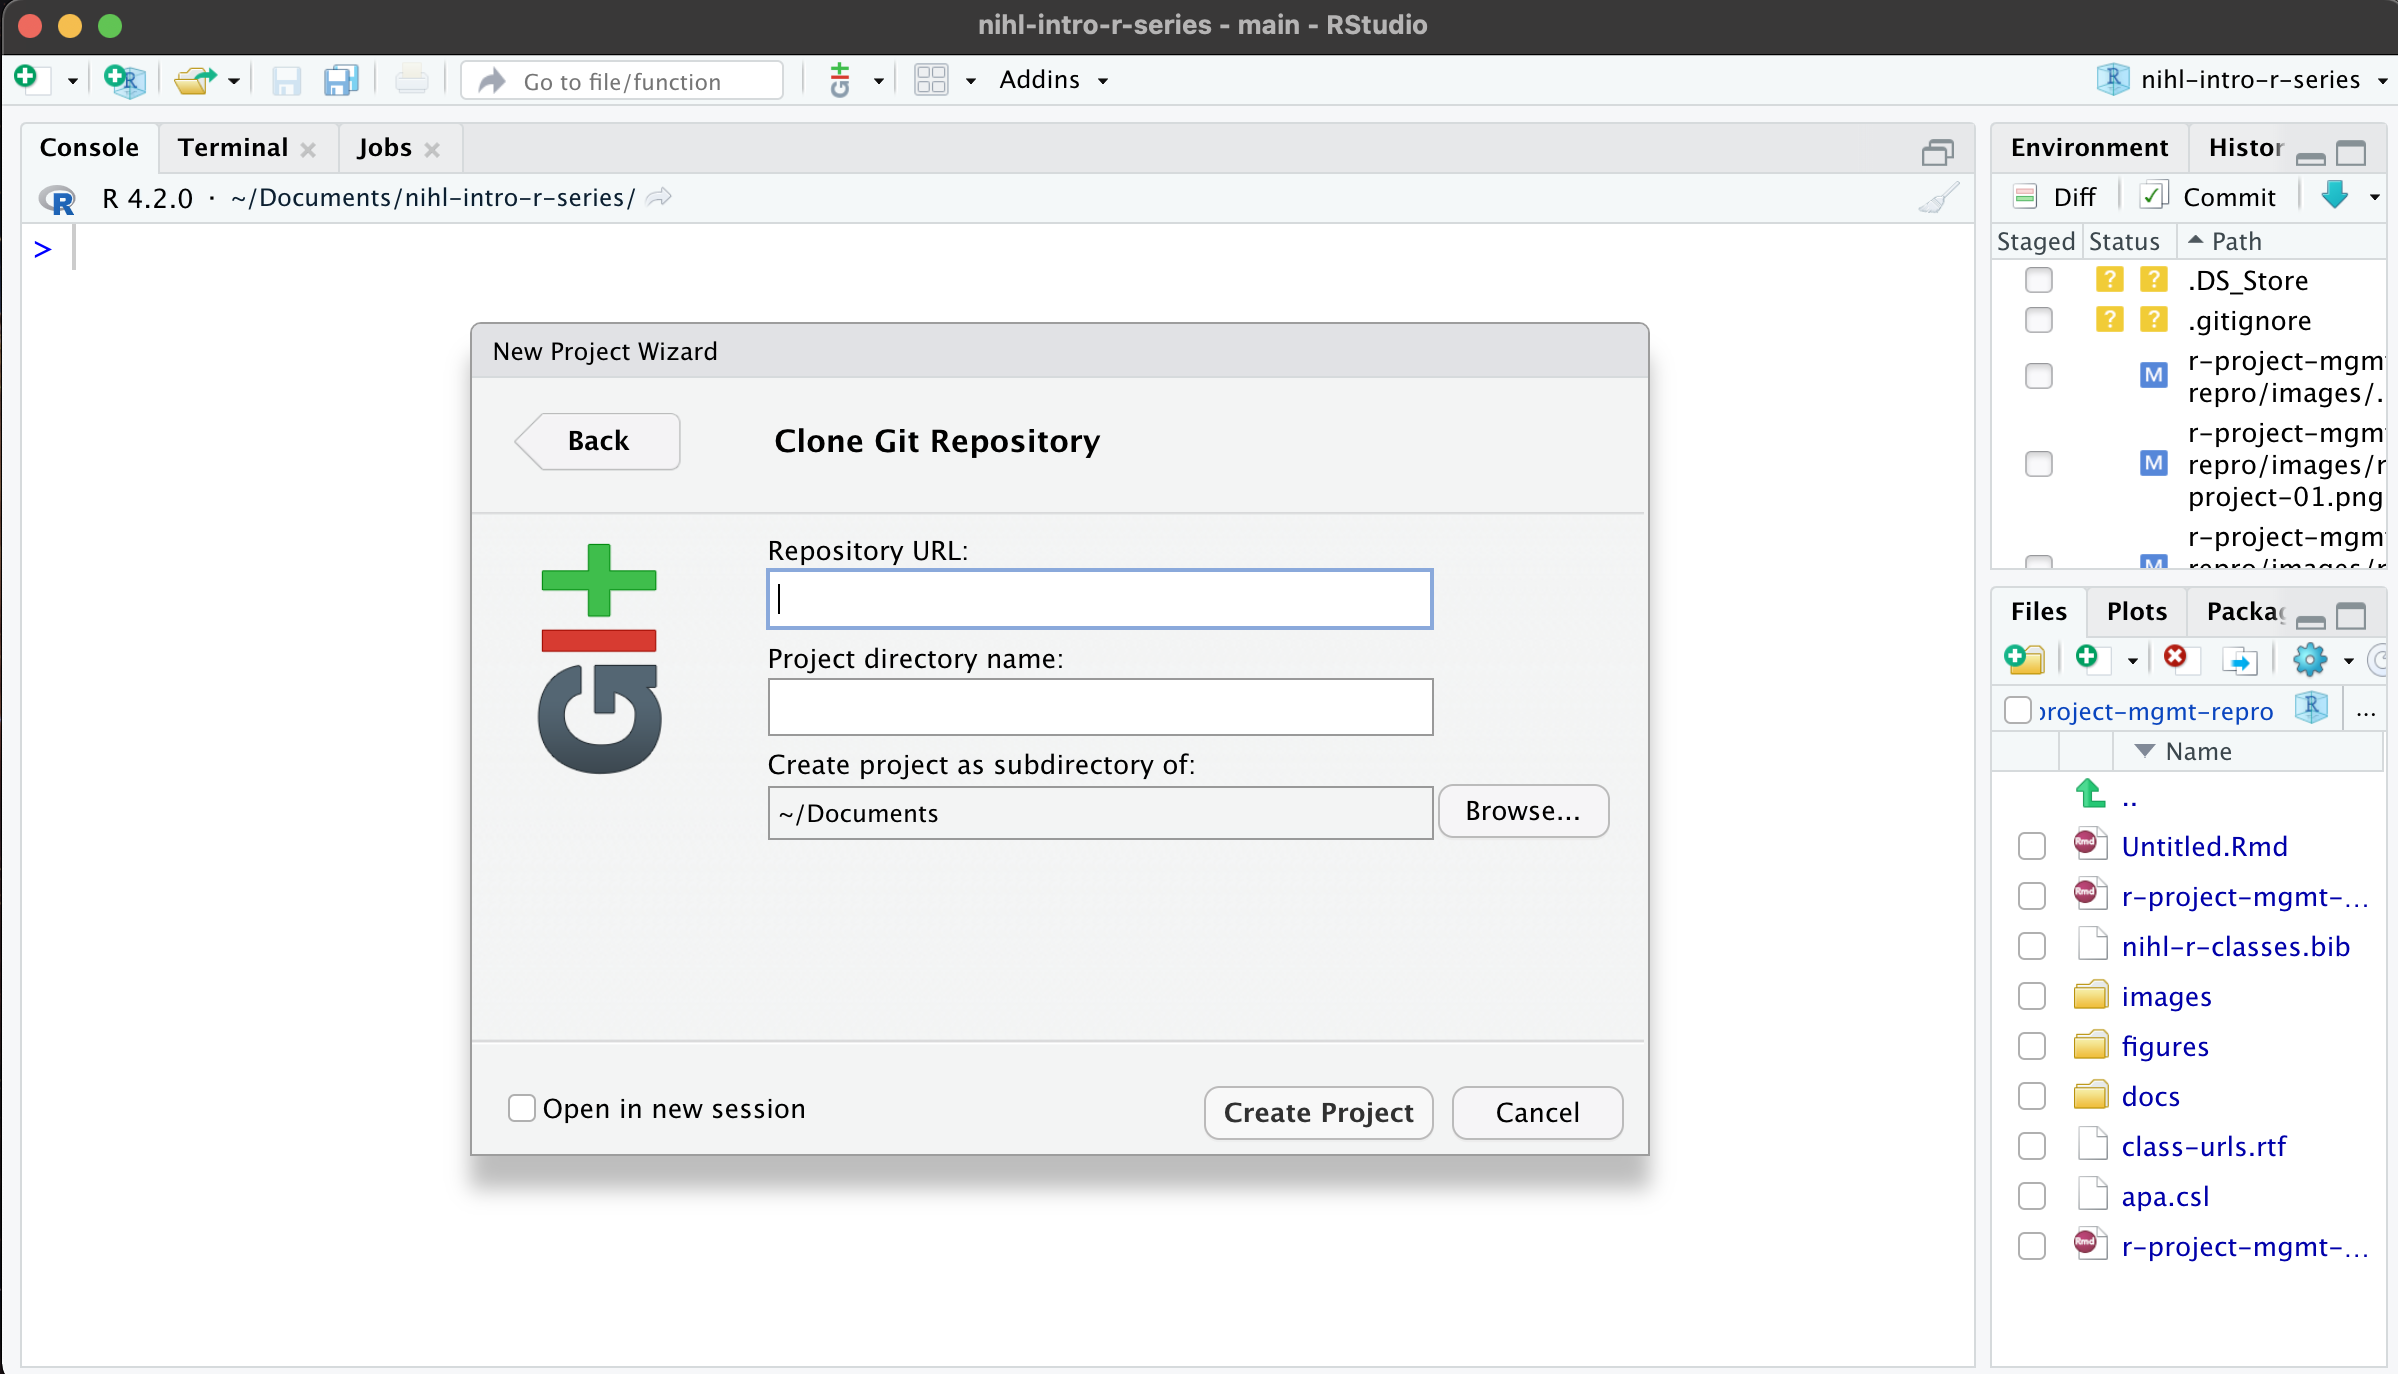
\includegraphics[width=4.5in,height=\textheight]{images/new-project-03.png}

Figure 11: Using a GitHub repository URL to create a new project

\begin{enumerate}
\def\labelenumi{\arabic{enumi}.}
\setcounter{enumi}{6}
\tightlist
\item
  Click \textbf{Create Project}. The screen will refresh as RStudio
  switches over to project view an downloads any data from GitHub
\end{enumerate}

\hypertarget{good-practices-for-managing-projects-in-rstudio}{%
\section{Good Practices for Managing Projects in
RStudio}\label{good-practices-for-managing-projects-in-rstudio}}

\hypertarget{sources}{%
\subsection{Sources}\label{sources}}

\href{Good\%20Practices\%20for\%20Managing\%20Projects\%20in\%20RStudio}{\textbf{Good
Practices for Managing Projects in RStudio}}

\hypertarget{project-organization-issues}{%
\subsection{Project Organization
Issues}\label{project-organization-issues}}

We often have stress points in our research that may become breaking
points, especially when it comes to working with collaborators,
returning to a project after a hiatus, or dealing with data and scripts.
Let's discuss three of those common stress points:

\hypertarget{filefolder-disorganization}{%
\subsubsection{File/folder
disorganization}\label{filefolder-disorganization}}

\begin{itemize}
\tightlist
\item
  You cannot find your files on your computer (or your cloud storage)
\item
  Multiple versions of files with names such as ``finaldraft\_4.txt''
\item
  Path issues when trying to run code
\item
  Reviewers or colleagues cannot re-run your code/analyses
\end{itemize}

\hypertarget{storage-and-sharing-issues}{%
\subsubsection{Storage and sharing
issues}\label{storage-and-sharing-issues}}

\begin{itemize}
\tightlist
\item
  Files are only saved to your computer and are vulnerable (or have
  already succumbed to computer/hard drive failure
\item
  When working with collaborators, they (or you) don't share the files
  needed
\item
  Files are shared via email attachments
\item
  Difficult to know if you have the latest version of documents
\end{itemize}

\hypertarget{losing-track-of-project-status}{%
\subsubsection{Losing track of project
status}\label{losing-track-of-project-status}}

\begin{itemize}
\tightlist
\item
  You cannot remember where you are in a project after being away for an
  extended period (or what you worked on the previous day\ldots no
  judgement)
\item
  You aren't sure what you should be working on next
\item
  You have various to-do notes spread across your office or home (or
  never write them down in the first place)
\end{itemize}

\hypertarget{discusion-points}{%
\subsection{Discusion Points}\label{discusion-points}}

To what extent do these stress points affect your research projects? Are
there additional issues that you've encountered that slow down or derail
your work due to issues with project management?

\hypertarget{project-filefolder-organization}{%
\subsection{Project File/Folder
Organization}\label{project-filefolder-organization}}

Although there is no ``best'' way to lay out a project, there are some
general principles to adhere to that will make project management
easier.

\hypertarget{practice-good-file-organization}{%
\subsection{Practice good
file-organization}\label{practice-good-file-organization}}

\href{http://swcarpentry.github.io/good-enough-practices-in-scientific-computing/}{Good
Enough Practices for Scientific Computing} gives the following
recommendations for project organization:

\begin{enumerate}
\def\labelenumi{\arabic{enumi}.}
\tightlist
\item
  Put each project in its own directory, which is named after the
  project.
\item
  Put text documents associated with the project in the doc directory.
\item
  Put raw data and metadata in the data directory, and files generated
  during cleanup and analysis in a results directory.
\item
  Put source for the project's scripts and programs in the src
  directory, and programs brought in from elsewhere or compiled locally
  in the bin directory.
\item
  Name all files to reflect their content or function.
\end{enumerate}

Additionally, we'd recommend to include README, LICENSE, and CITATION
files! Additionaly recommendations for projects and creating folders is
covered in the Introduction to R and Rstudio class. Class handouts are
available upon request.

\hypertarget{practices-for-naming-files}{%
\subsection{Practices for Naming
Files}\label{practices-for-naming-files}}

\hypertarget{machine-readable}{%
\subsubsection{Machine-readable}\label{machine-readable}}

No spaces, unsupported punctuation, accented characters, or
case-sensitive file names

Deliberate use of delimiters (i.e.~for splitting file names)

Consistently use the same delimiters: \texttt{data-analyses-fig1.R} as
an example

\hypertarget{human-readable}{%
\subsubsection{Human-readable}\label{human-readable}}

Name contains brief description of content:
i.e.~\texttt{data-analyses-fig1.R}

\hypertarget{ordering-files}{%
\subsubsection{Ordering Files}\label{ordering-files}}

Use chronological or logical order. With chronological, file name starts
with date.

\begin{itemize}
\item
  i.e.~\texttt{2022-01-01\_data\_analyses.R}
\item
  Use \href{https://en.wikipedia.org/wiki/ISO_8601}{ISO 8601 date
  standard}
\item
  \textbf{logical}: filename starts with a number or keyword/number
  combo.

  \begin{itemize}
  \item
    i.e.~\texttt{01\_data\_preprocessing.R} \emph{see code directory}
  \item
    i.e.~\texttt{CC-101\_1\_data.csv} \emph{see data directory}
  \end{itemize}
\end{itemize}

Adapted from
\url{https://datacarpentry.org/rr-organization1/01-file-naming/index.html}.
For more tips on file naming, check:
\href{https://www.library.ucsb.edu/sites/default/files/dls-n01-2021-filenaming.pdf}{The
Dos and Don'ts of File Naming}.

\hypertarget{working-with-r-markdown-files}{%
\section{Working with R Markdown
Files}\label{working-with-r-markdown-files}}

R Markdown provides an authoring framework for data science. You can use
a single R Markdown file to both

\begin{itemize}
\item
  save and execute code
\item
  generate high quality reports that can be shared with an audience
\end{itemize}

R Markdown documents are fully reproducible and support dozens of static
and dynamic output formats.

\hypertarget{installation}{%
\subsection{Installation}\label{installation}}

Like the rest of R, R Markdown is free and open source. You can install
the R Markdown package from CRAN with:

\begin{verbatim}
install.packages("rmarkdown")
\end{verbatim}

You will also need to install the \href{http://yihui.name/knitr/}{knitr}
package. Knitr is a general-purpose tool for dynamic report generation
in R using Literate Programming techniques.

\begin{verbatim}
install.packages("knitr")
\end{verbatim}

There are a number of packages that are required for \texttt{rmarkdown}
and \texttt{knitr}, these should install automatically.

\hypertarget{getting-started}{%
\subsubsection{Getting Started}\label{getting-started}}

This \href{https://rmarkdown.rstudio.com/lesson-1.html}{page} provides a
nice overview of R markdown the top provide examples of R Markdown
documents, as well as an in depth discussion of various R Markdown
topics.

You may also find the following resources helpful:

\begin{itemize}
\item
  \href{https://github.com/rstudio/cheatsheets/raw/main/rmarkdown-2.0.pdf}{The
  R Markdown Cheatsheet}
\item
  \href{https://www.rstudio.com/wp-content/uploads/2015/03/rmarkdown-reference.pdf}{The
  R Markdown Reference Guide}
\item
  \href{https://bookdown.org/yihui/rmarkdown-cookbook/}{R Markdown
  Cookbook}
\end{itemize}

\hypertarget{writing-and-styling-rmd-documents}{%
\subsection{Writing and Styling Rmd
Documents}\label{writing-and-styling-rmd-documents}}

Let us create a new document by navigating to
\texttt{File\ \textgreater{}\ New\ File\ \textgreater{}\ R\ Markdown}.

\begin{itemize}
\item
  Add the title \texttt{Code-Chunk-Test}.
\item
  Add your name as author
\item
  Select ``Use current date when rendering documents''
\end{itemize}

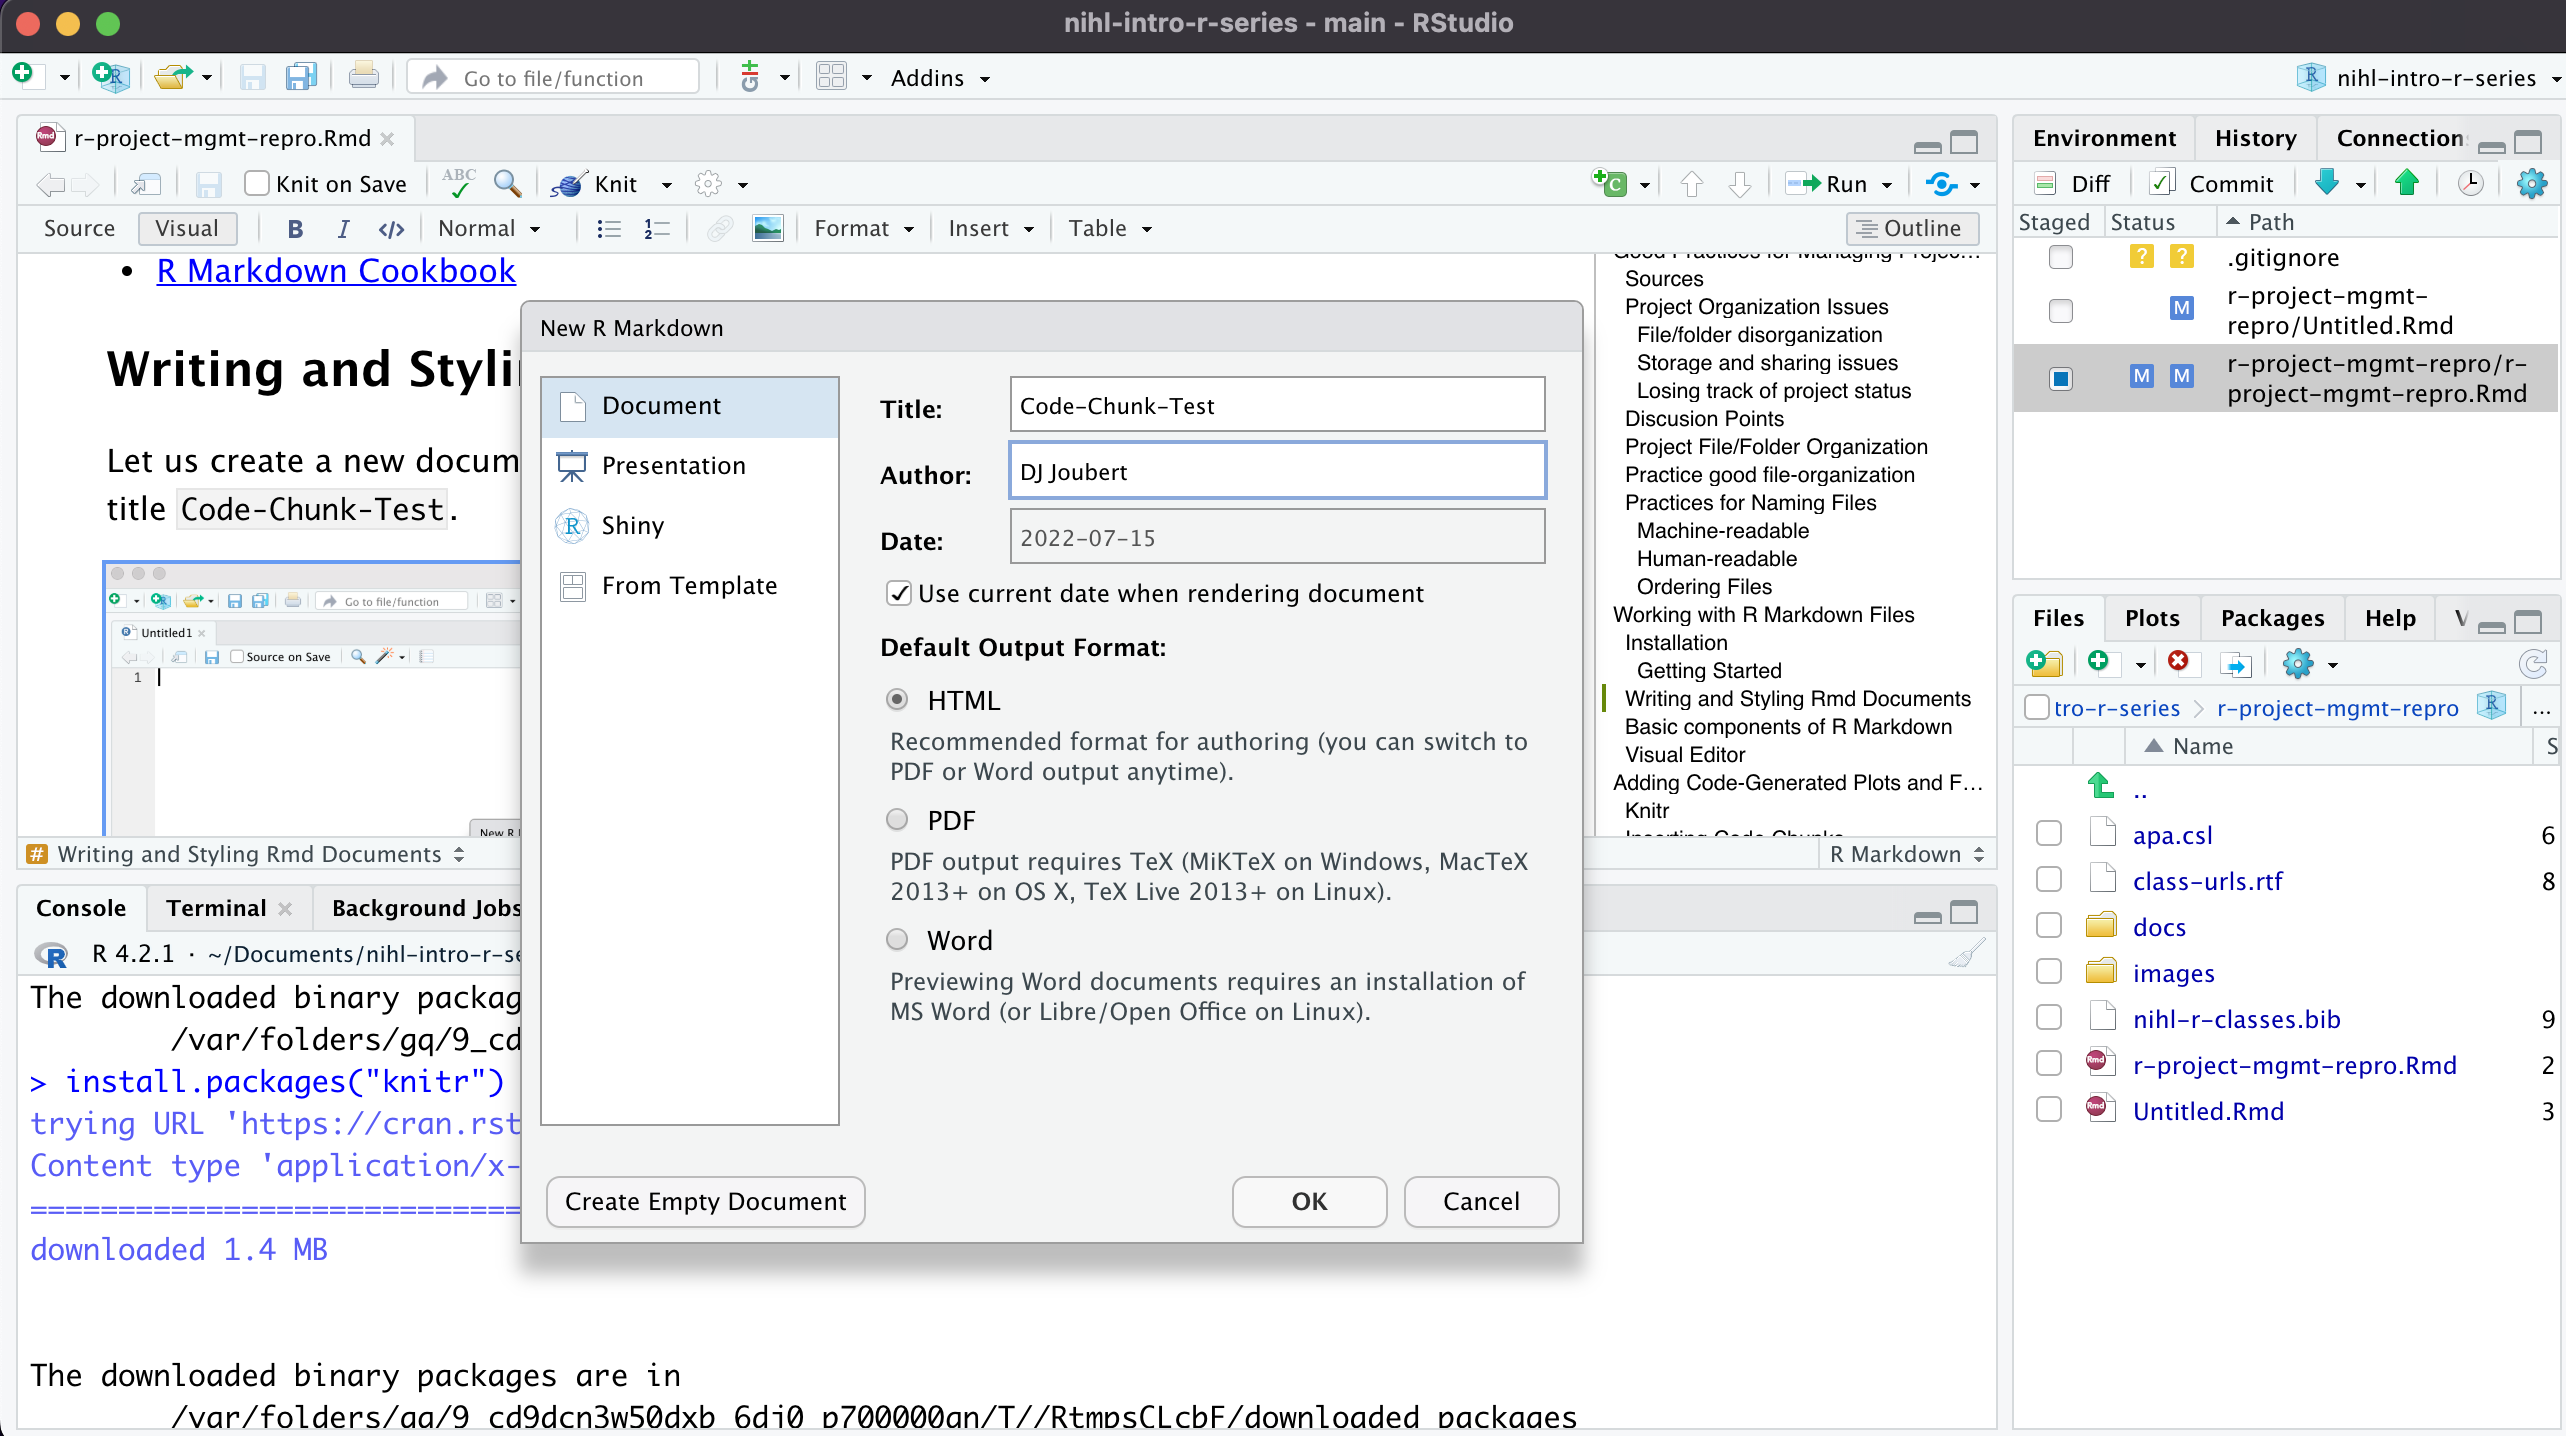
\includegraphics[width=6.5in,height=\textheight]{images/02-name-new-rmd.png}

Figure 8: Creating a new markdown document

If you scroll down the doc that you just created you can see that the
RMD file is already populated with text and code.

Let's first delete the generic text because we don't need it at this
point (all except the first code chunk that is - we'll get back to that
in a second).

\hypertarget{basic-components-of-r-markdown}{%
\subsection{Basic components of R
Markdown}\label{basic-components-of-r-markdown}}

The initial chunk of text (header) contains instructions for R to
specify what kind of document will be created, and the options chosen.
You can use the header to give your document a title, author, date, and
tell it what type of output you want to produce.

\begin{verbatim}
---
title: "Introduction to R Markdown"
author: "Doug Joubert"
date: "2022-07-18"
output: html_document
---
\end{verbatim}

You can delete any of those fields if you don't want them included. The
double-quotes aren't strictly \emph{necessary} in this case. They're
mostly needed if you want to include a colon in the title.

Note that you have the option to select \emph{Use the current date when
rendering the document}. If you choose so, this will generate the date
dynamically each time you knit your document and replace the rmd
creation date with the inline R expression:

2022-07-18

You may also consider exploring changing date formats
\href{https://bookdown.org/yihui/rmarkdown-cookbook/update-date.html}{following
these tips}.

\hypertarget{source-editor}{%
\subsection{Source Editor}\label{source-editor}}

The image below displays the default R Markdown template in the ``source
editor'' mode. Notice the symbols scattered throughout the text (\#, *,
\textless\textgreater). Those are examples of R Markdown syntax, which
is a flavor of Markdown syntax, an easy and quick, human-readable markup
language for document styling.

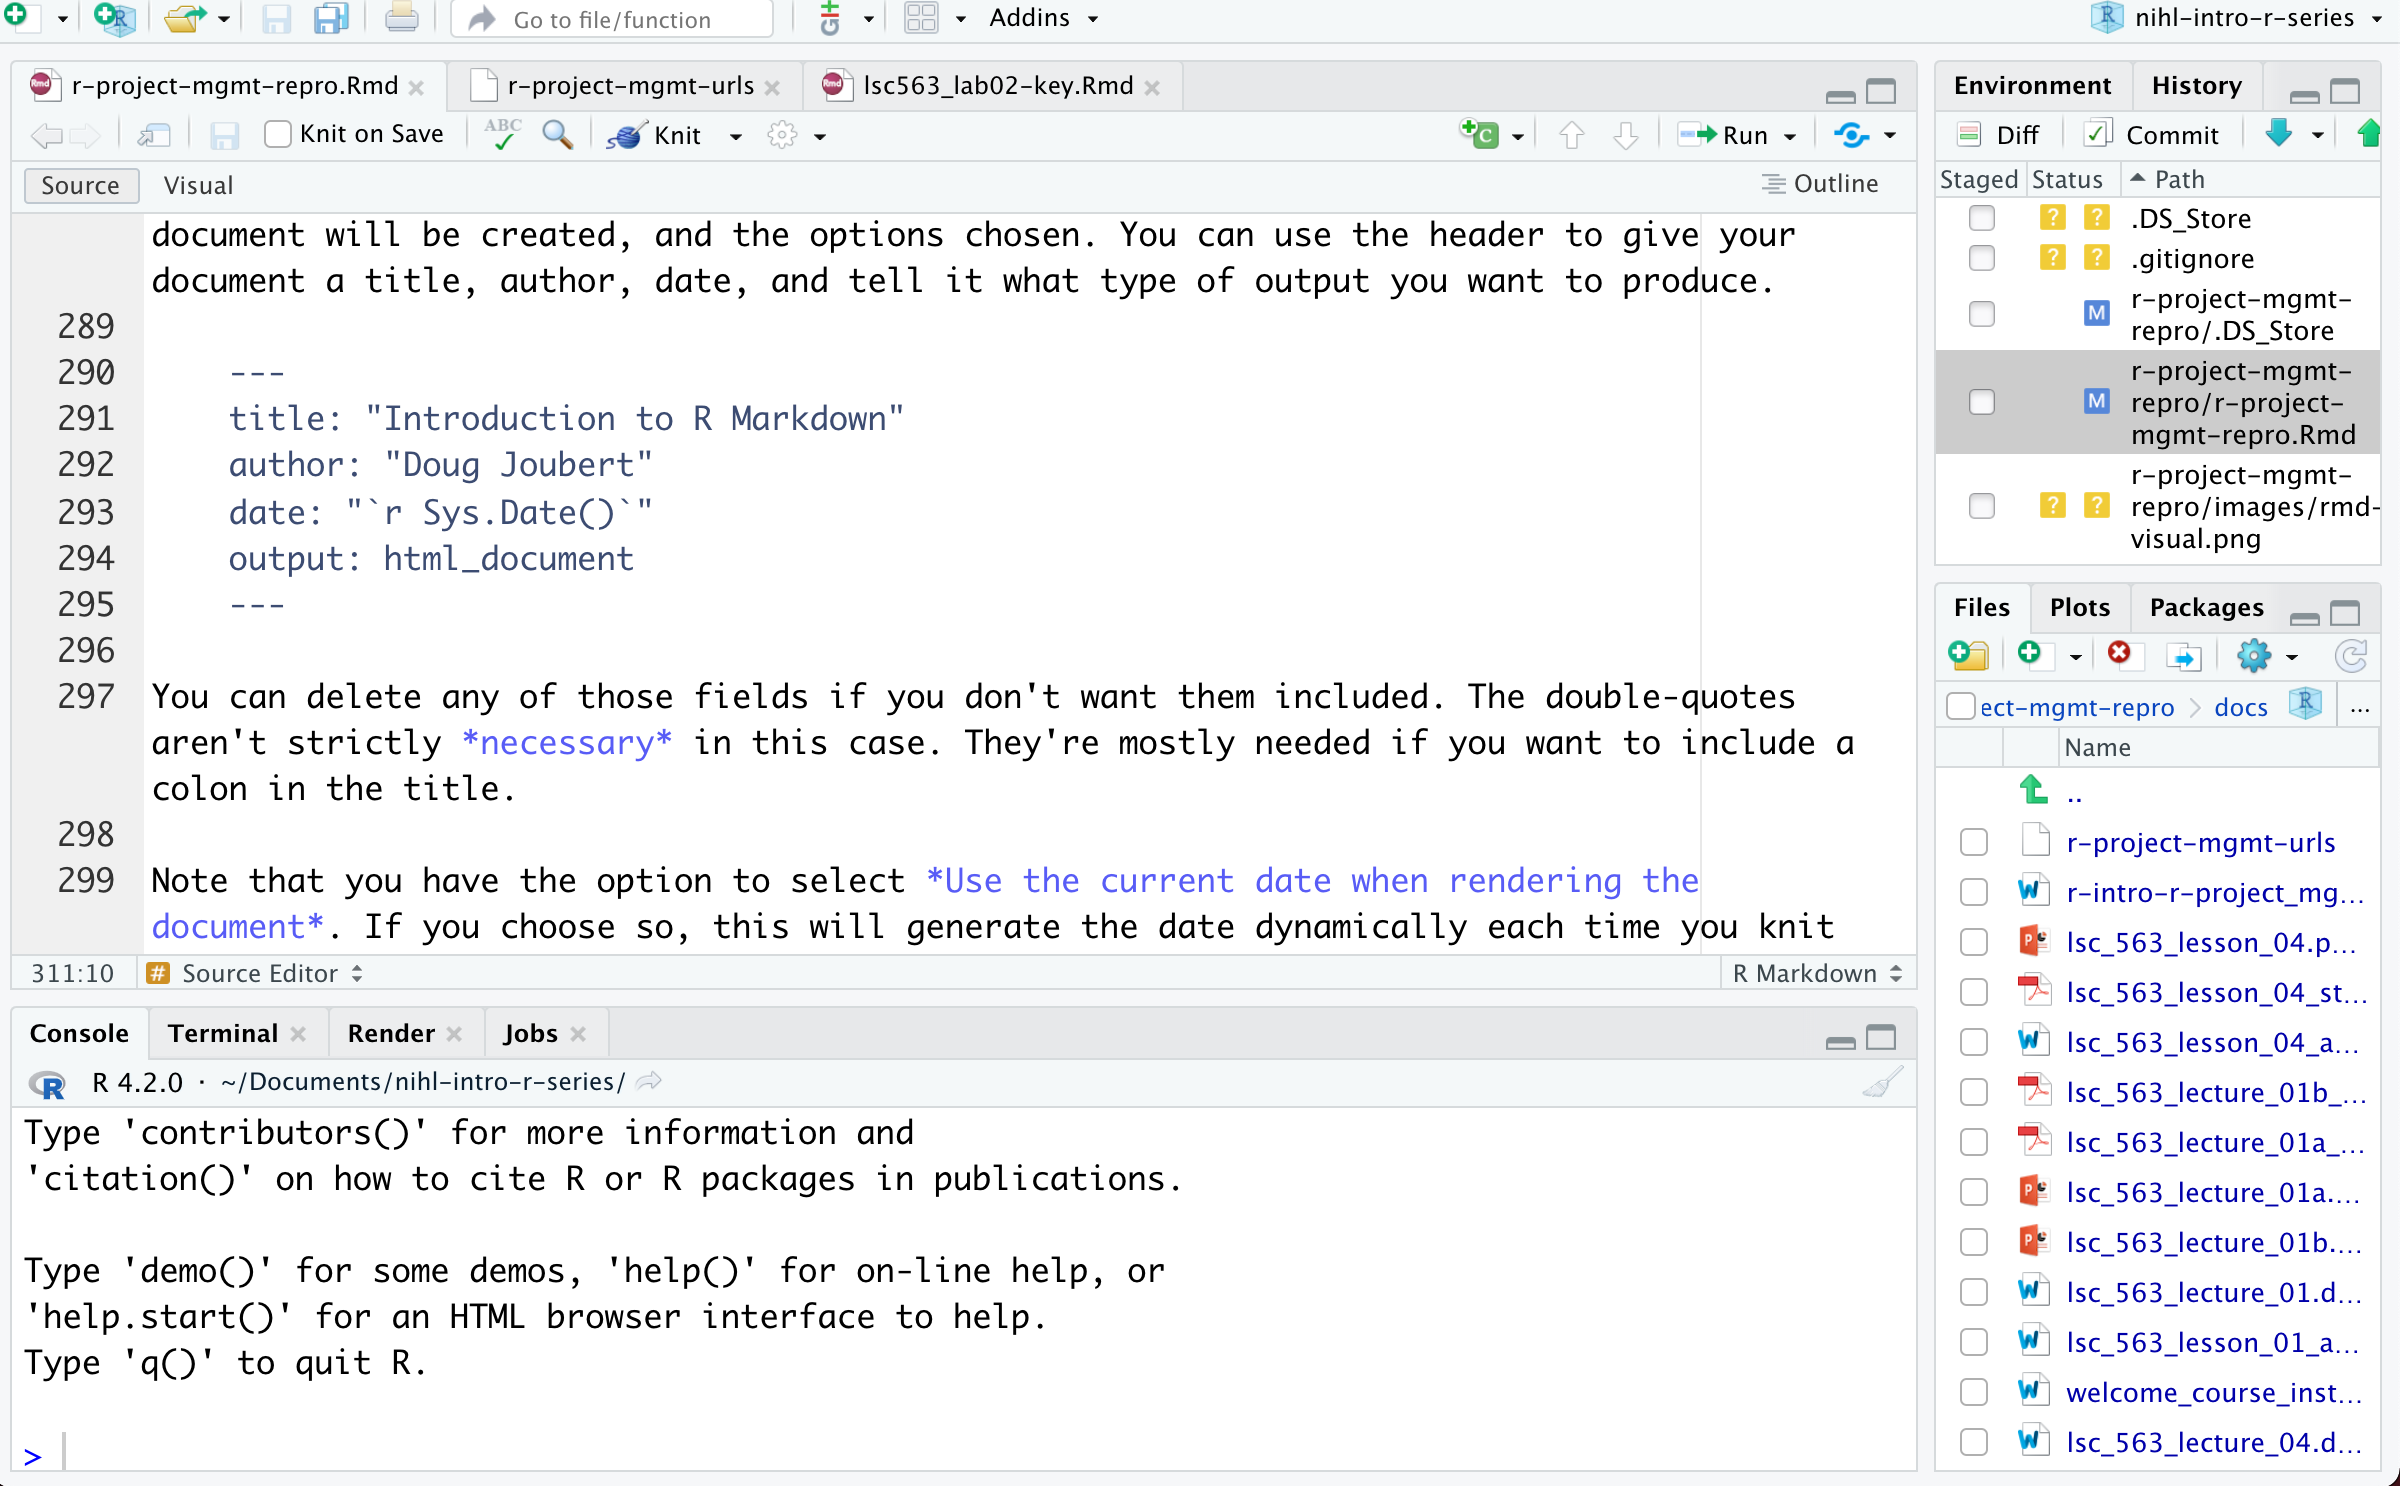
\includegraphics[width=6.5in,height=\textheight]{images/02-rmd-new-template.png}

Figure 9: Creating an RMD file in RStudio.

\hypertarget{visual-editor}{%
\subsection{Visual Editor}\label{visual-editor}}

RStudio released a new major update to their IDE in January 2020, which
includes a new ``visual editor'' for R Markdown to supplement their
original editor (which we will call the source editor) for authoring
with R Markdown syntax.

The new visual editor is friendlier with a graphical user interface
similar to Word or Google docs that lets you choose styling options from
the menu (before you had to either have the R Markdown code memorized or
look it up for each of your styling choices). Another major benefit is
that the new editor renders the R Markdown styling in real time so you
can preview your paper before rendering to your output format. The image
below is displaying the same document using the visual editor.

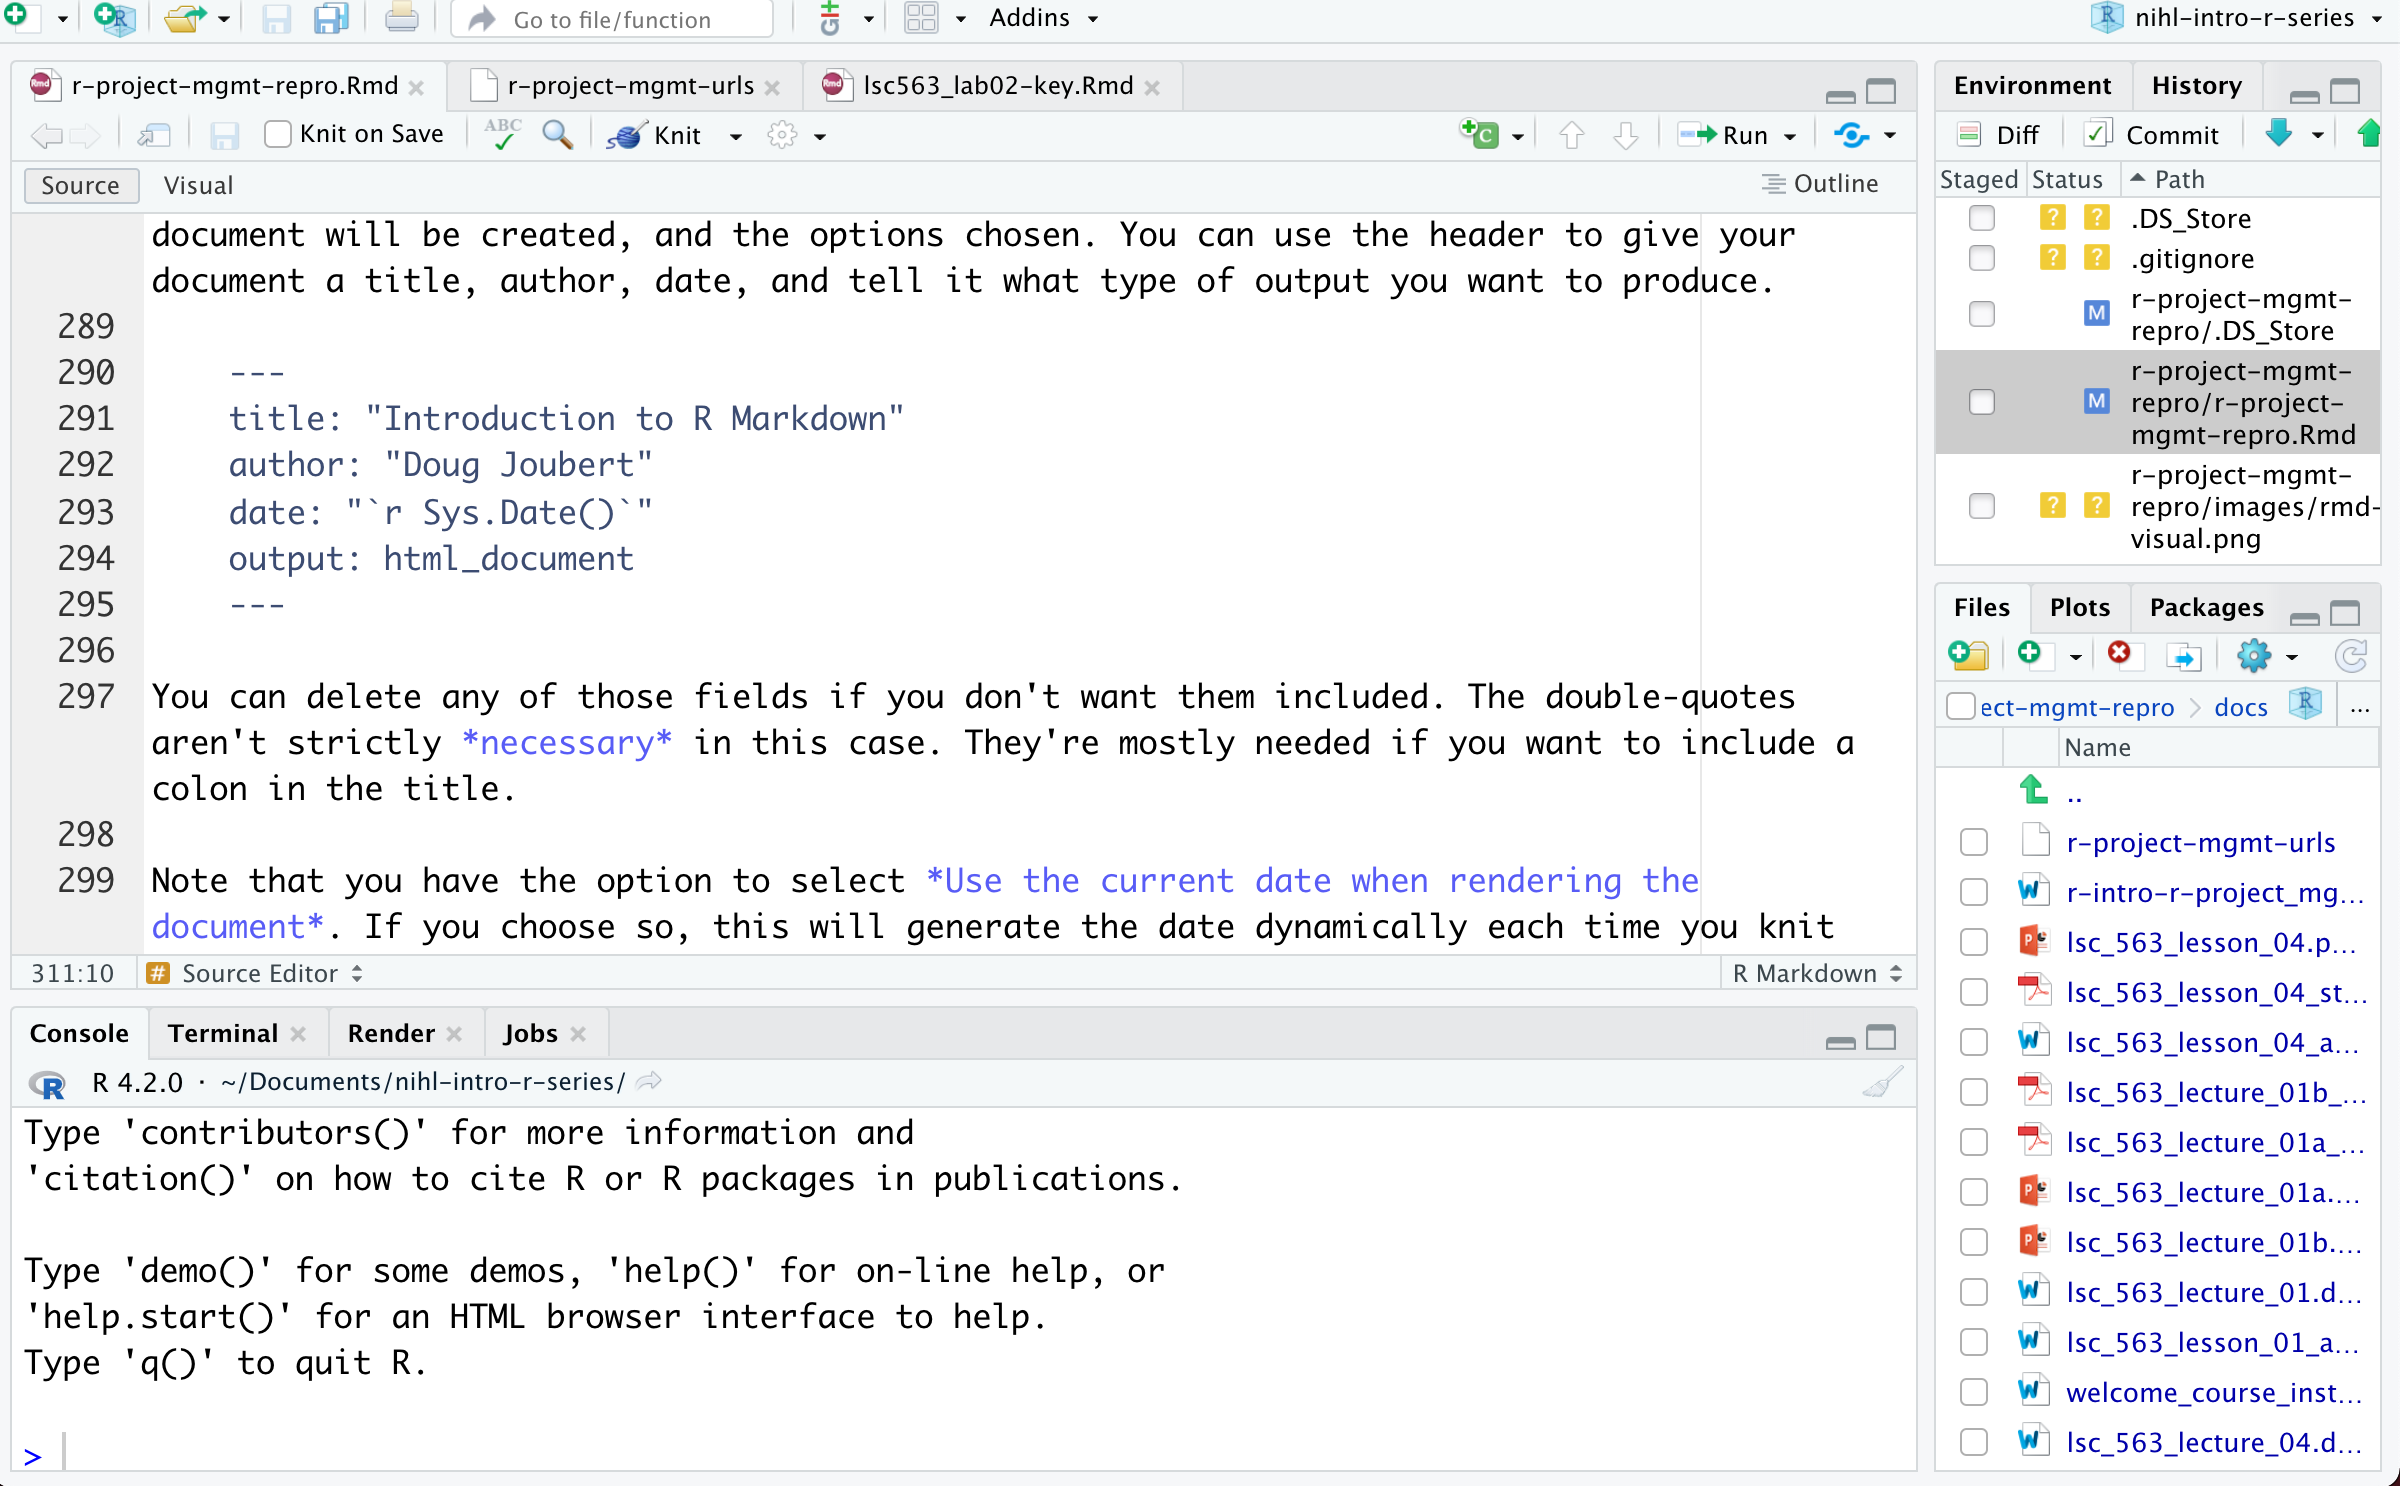
\includegraphics[width=6.5in,height=\textheight]{images/02-rmd-new-template.png}

Figure 10: Source/Visual options for markdown

On a PC the visual editor is accessible through a small button on the
far right side of the script/document pane in RStudio. The icon is a
protractor, but from further away it just looks like a squiggly ``A''.

On a Mac there are Source/Visual tabs on the Menu panel

\hypertarget{adding-code-generated-plots-and-figures}{%
\section{Adding Code-Generated Plots and
Figures}\label{adding-code-generated-plots-and-figures}}

There are two main ways to process code with Knitr in R Markdown
documents:

\begin{enumerate}
\def\labelenumi{\arabic{enumi}.}
\item
  Code Chunks
\item
  Inline Code
\end{enumerate}

\hypertarget{inserting-code-chunks}{%
\subsection{Inserting Code Chunks}\label{inserting-code-chunks}}

Code chunks are better when you need to do something more sophisticated
with your code, such as building plots or tables. They also incorporate
syntax which allows modifications to how that code is rendered and
styled in your final output. We'll learn more about that as we walk
through the ``anatomy'' of a code chunk.

\hypertarget{basic-anatomy-of-the-code-chunk}{%
\subsection{Basic Anatomy of the Code
Chunk}\label{basic-anatomy-of-the-code-chunk}}

You can quickly insert chunks like these into your file with:

\begin{itemize}
\item
  the keyboard shortcut Ctrl + Alt + I (OS X: Cmd + Option + I)
\item
  the Add Chunk command in the editor toolbar
\item
  or by typing the chunk delimiters \{r\} and ```.
\end{itemize}

The most basic (and empty) code chunk looks like this:

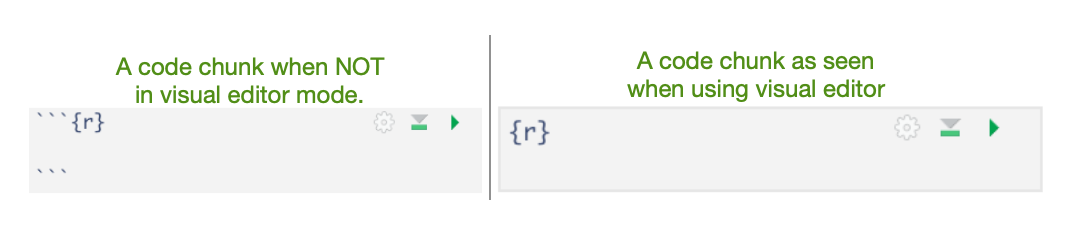
\includegraphics[width=6.5in,height=\textheight]{images/blank-code-chunk.png}

Although I am demostrating using R in this workshop, it's possible to
use other programming or markup languages. For example, we have seen
that we can use LaTeX code for equations. You can also use python and a
handful of other languages.

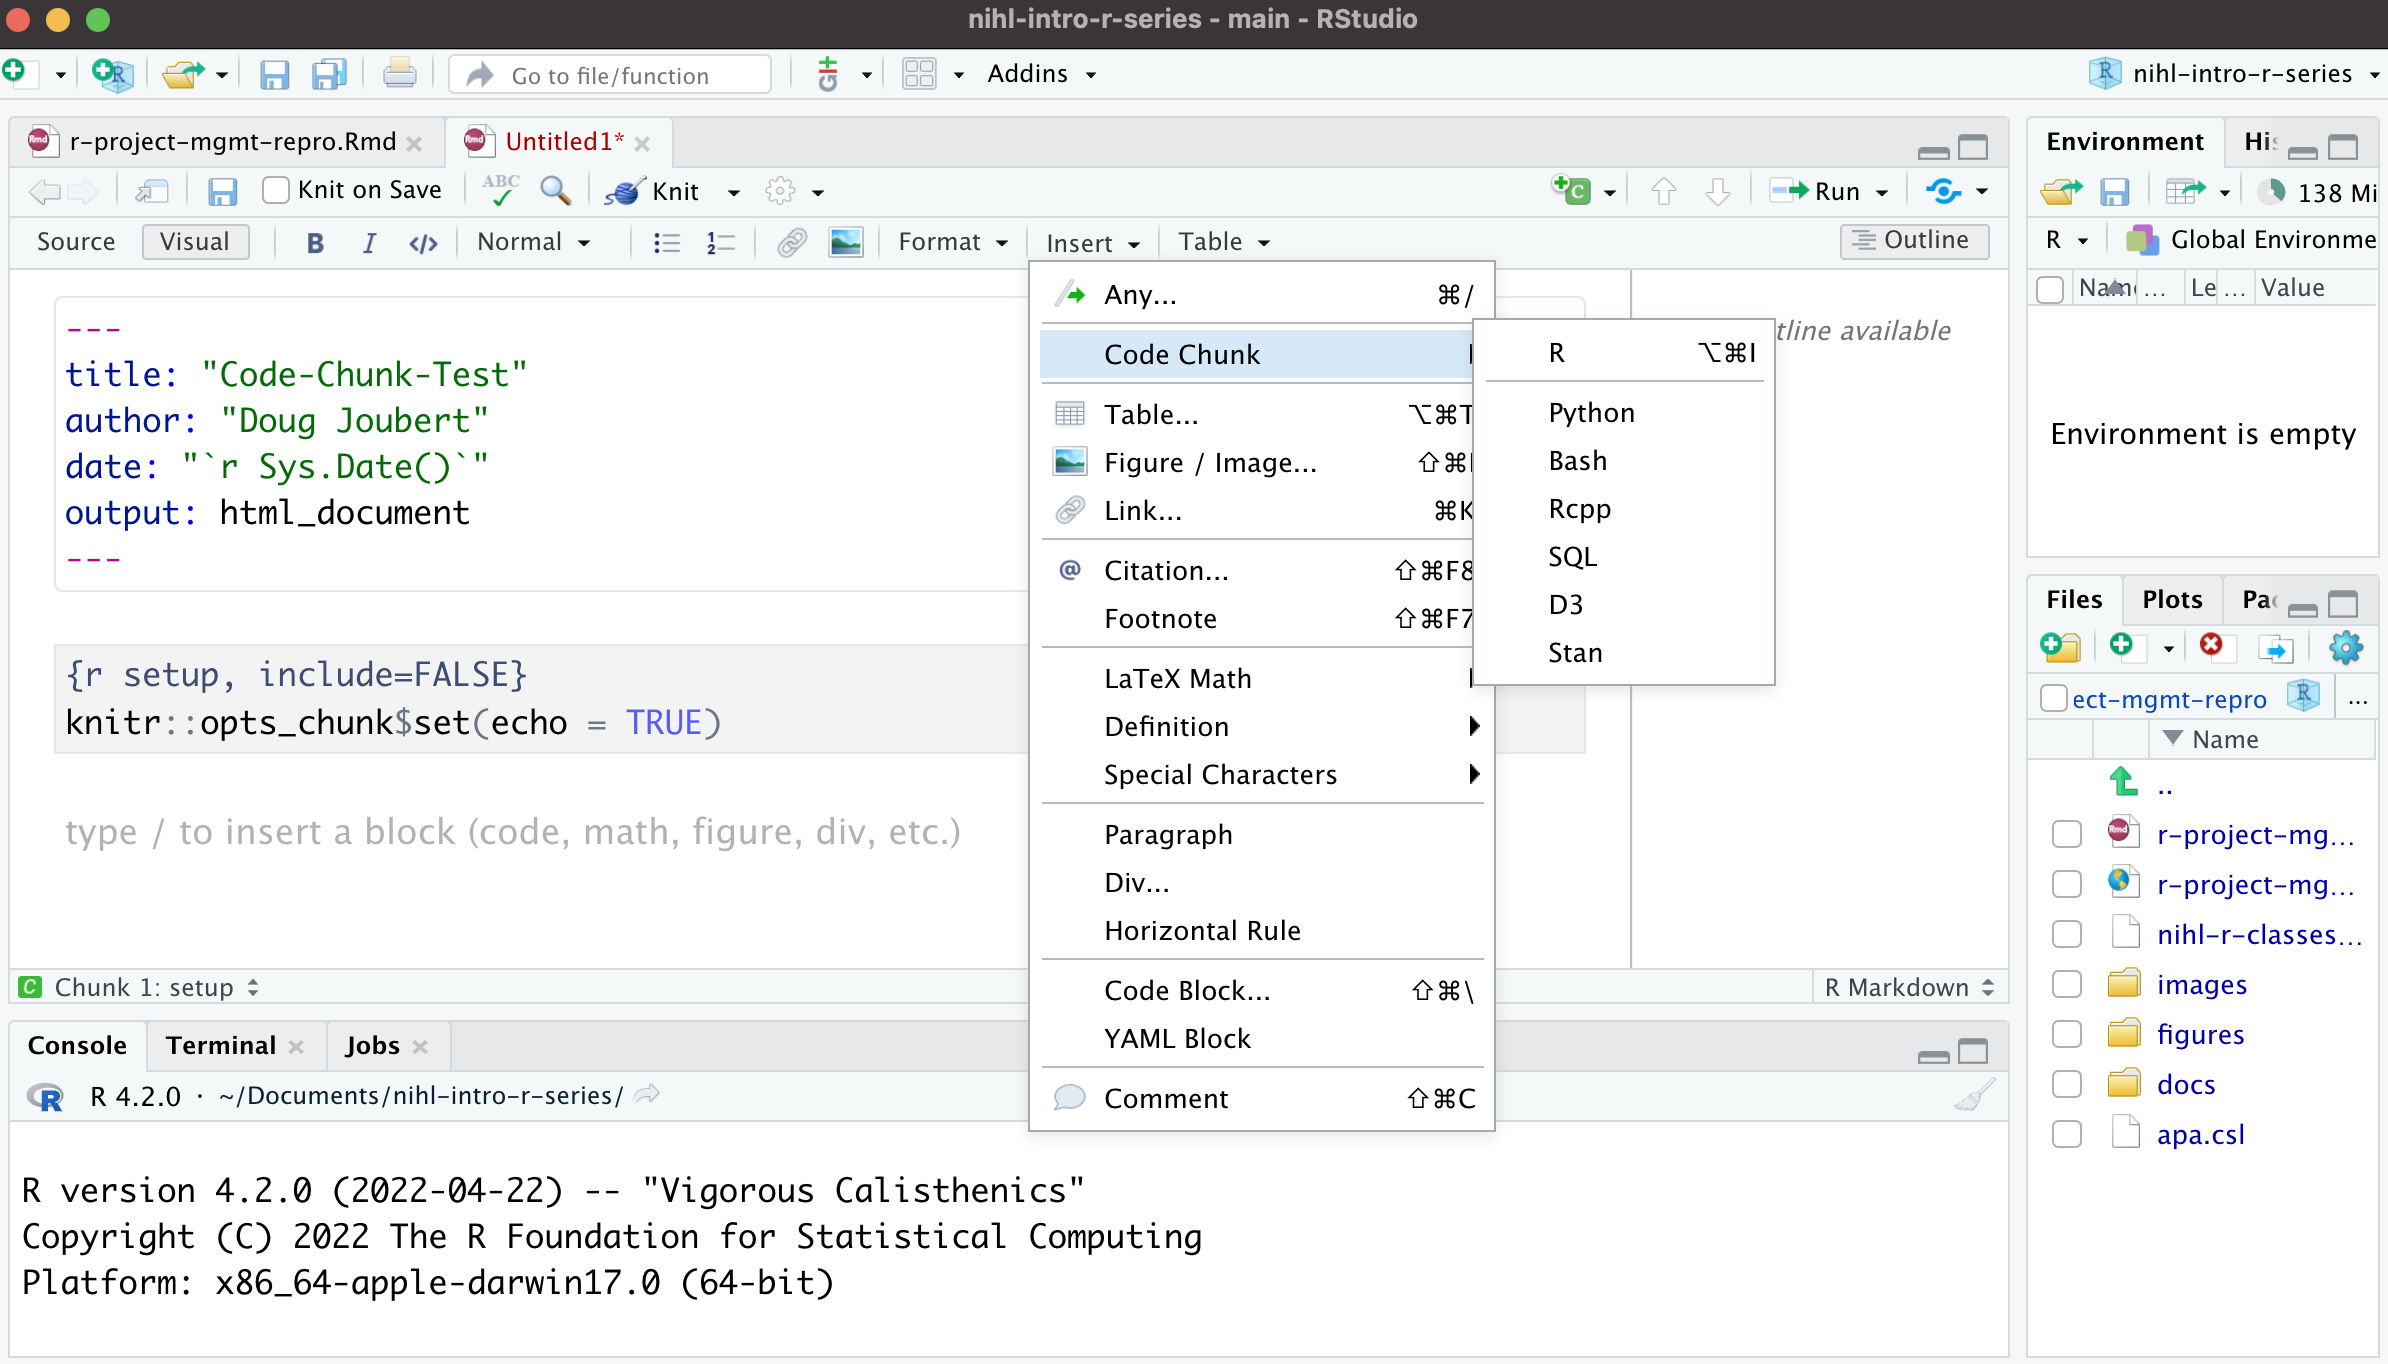
\includegraphics[width=6.5in,height=\textheight]{images/code-chunk-other.png}

Figure 11: Code options available in R-markdown.

There's a button you can use in the RStudio menu to generate the code
chunks automatically. Automatic code chunk generation is available for
several other languages as well. Also, you can use the keyboard shortcut
\texttt{ctrl}+\texttt{alt}+\texttt{i} for Windows and
\texttt{command}+\texttt{option}+\texttt{i} for Mac. As you can see in
Figure 12, the console is blank because we have not executed/run the
code chunk. Let us enter the following read statement into our first
code chunk:

\texttt{\#\ This\ is\ a\ example\ of\ a\ code\ chunk\ to\ read\ in\ some\ data}

\texttt{library(tidyverse)}

\texttt{read\_data\ \textless{}-\ "../raw-data/combined.csv"}

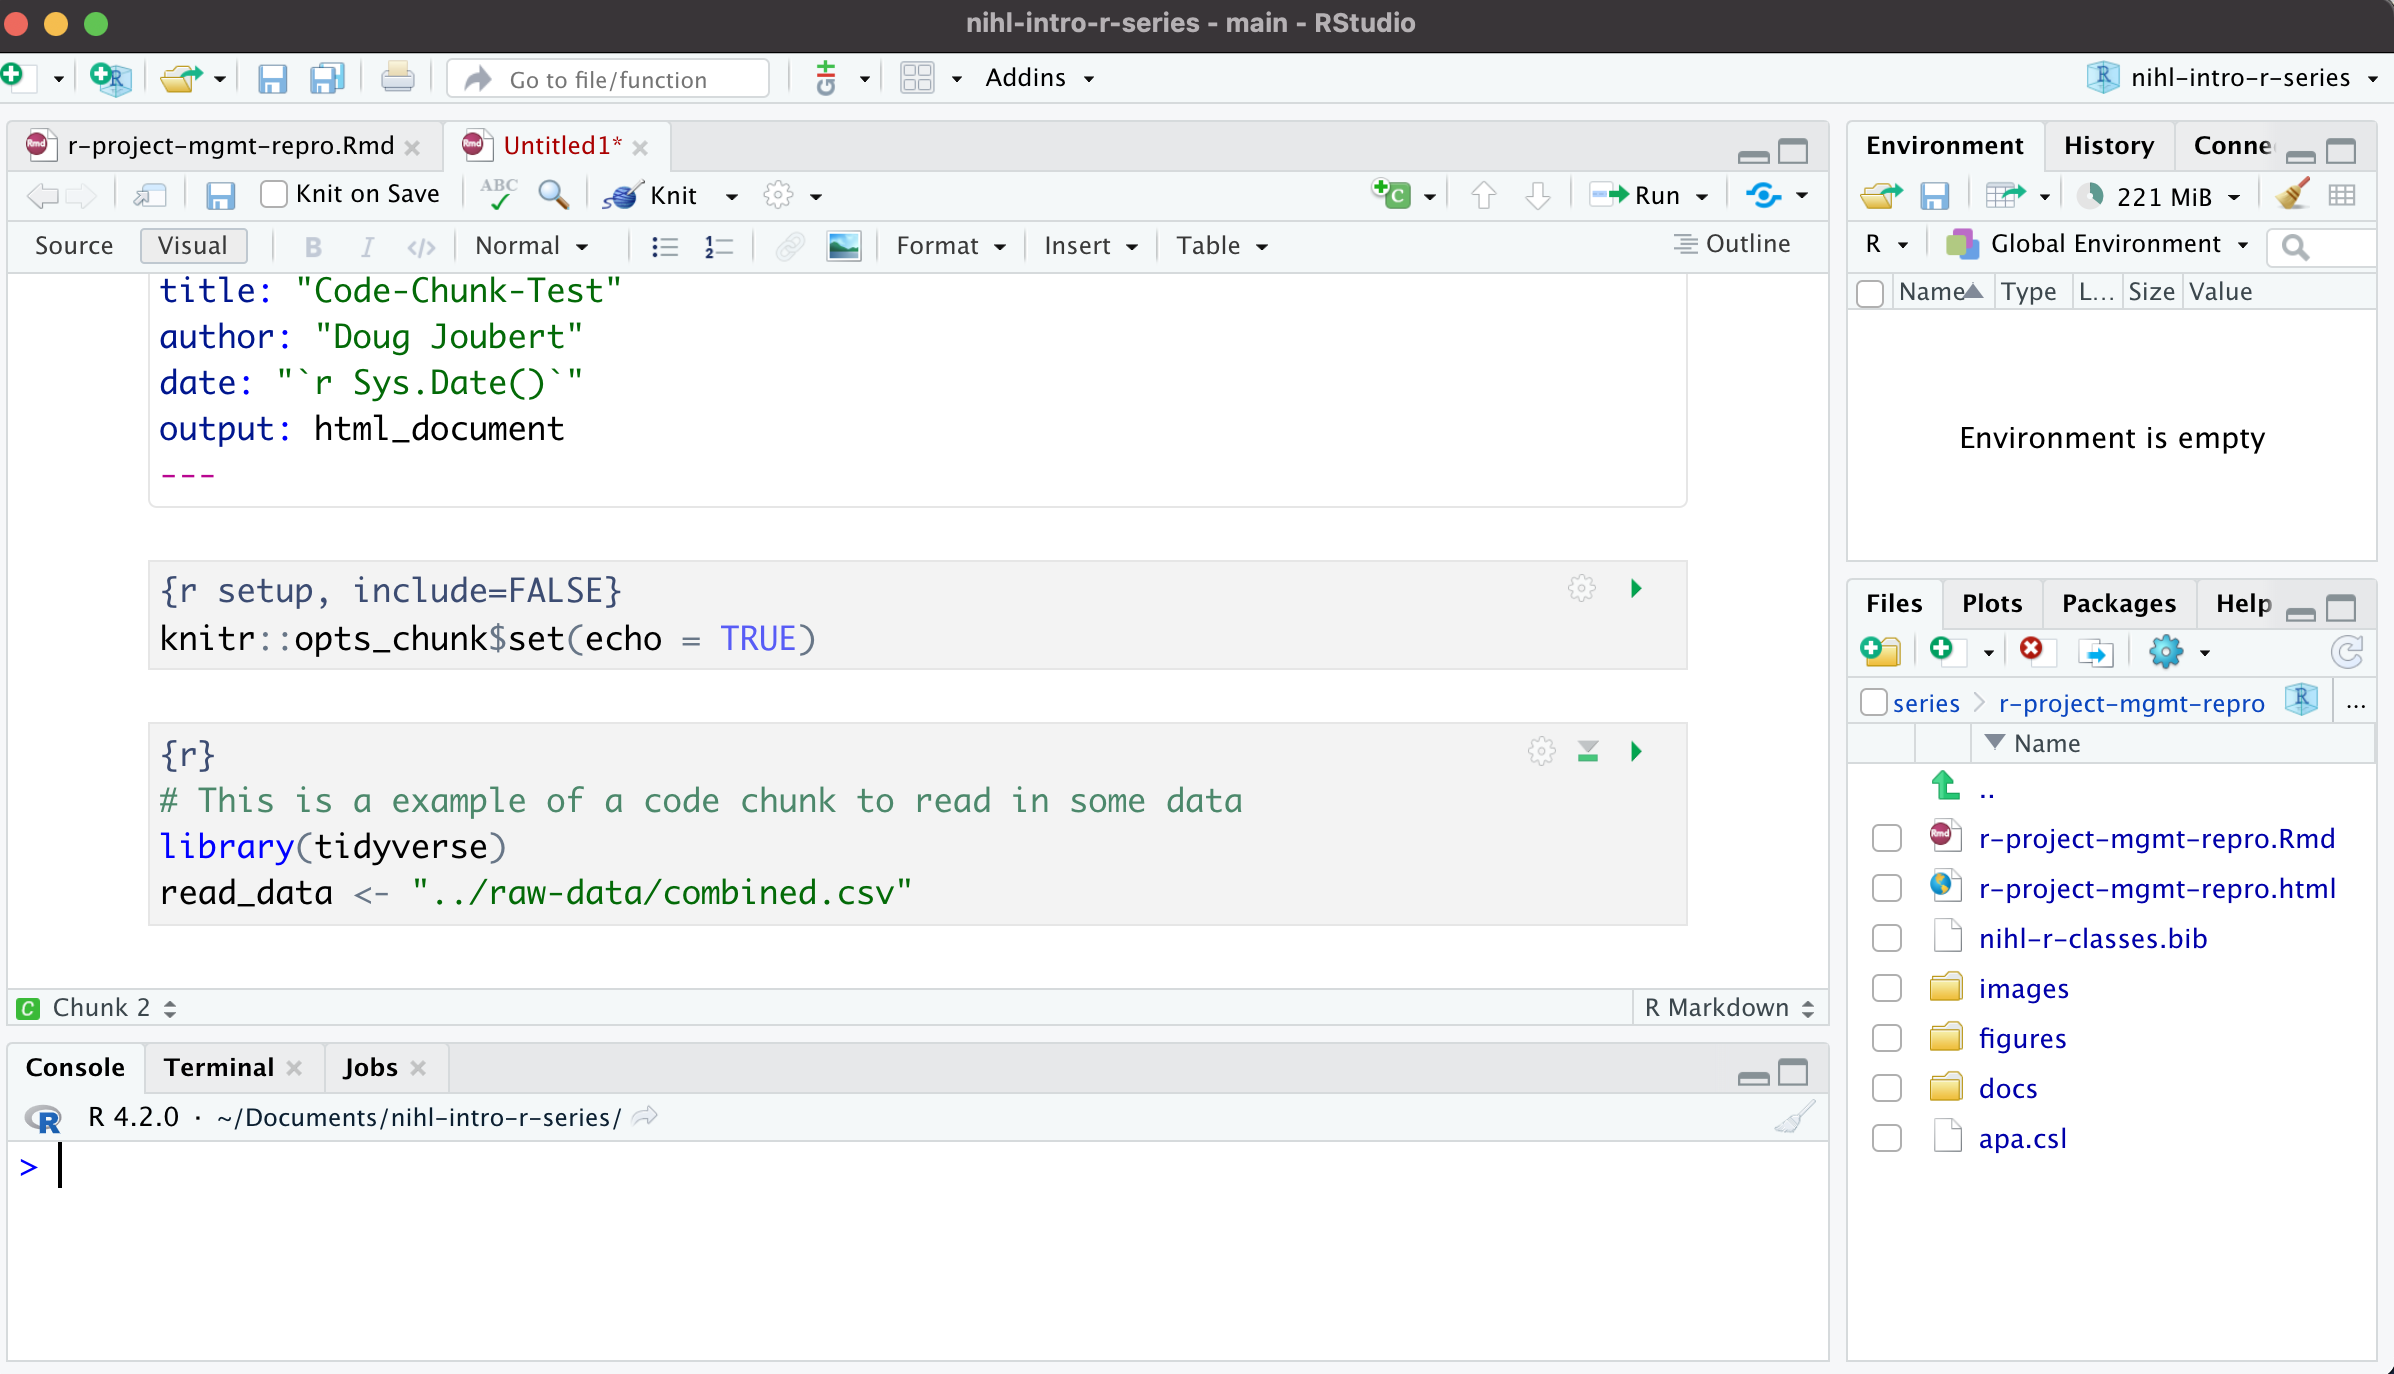
\includegraphics[width=6.5in,height=\textheight]{images/code-chunk-script.png}

Figure 12: Code chunk in R-markdown.

\hypertarget{run-the-code-in-a-code-chunk}{%
\subsection{Run the code in a code
chunk}\label{run-the-code-in-a-code-chunk}}

There are 3 main options for running and debugging code that don't
require us to wait for the file to render.

\begin{enumerate}
\def\labelenumi{\arabic{enumi})}
\tightlist
\item
  Run from code chunk (green play button on the right top corner). This
  allows us to run one specific code chunk {[}Figure13{]}.
\end{enumerate}

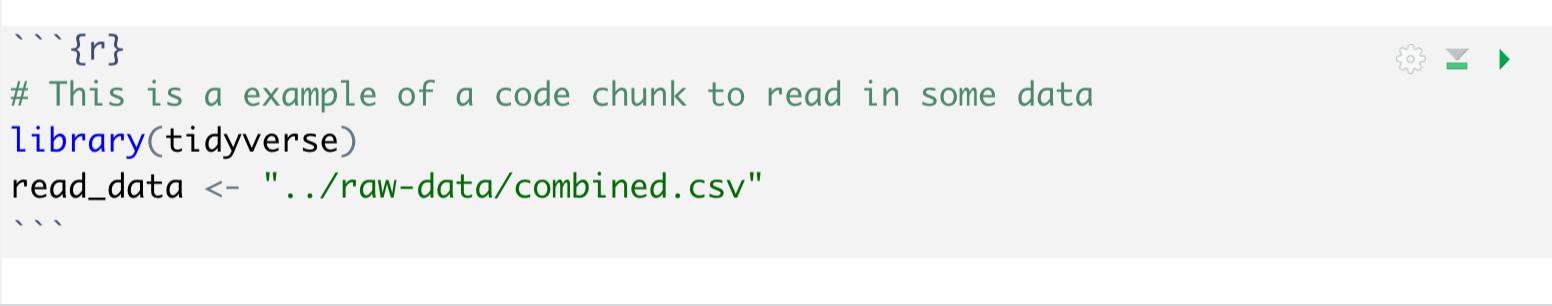
\includegraphics[width=6.5in,height=\textheight]{images/code-chunk-run-01.png}

Figure 13: Running a code chunk from the code-box.

\begin{enumerate}
\def\labelenumi{\arabic{enumi}.}
\setcounter{enumi}{1}
\tightlist
\item
  Run menu, which gives more options for running code chunks including
  the current one, the next one, all chunks, etc {[}Figure 14{]}.
\end{enumerate}

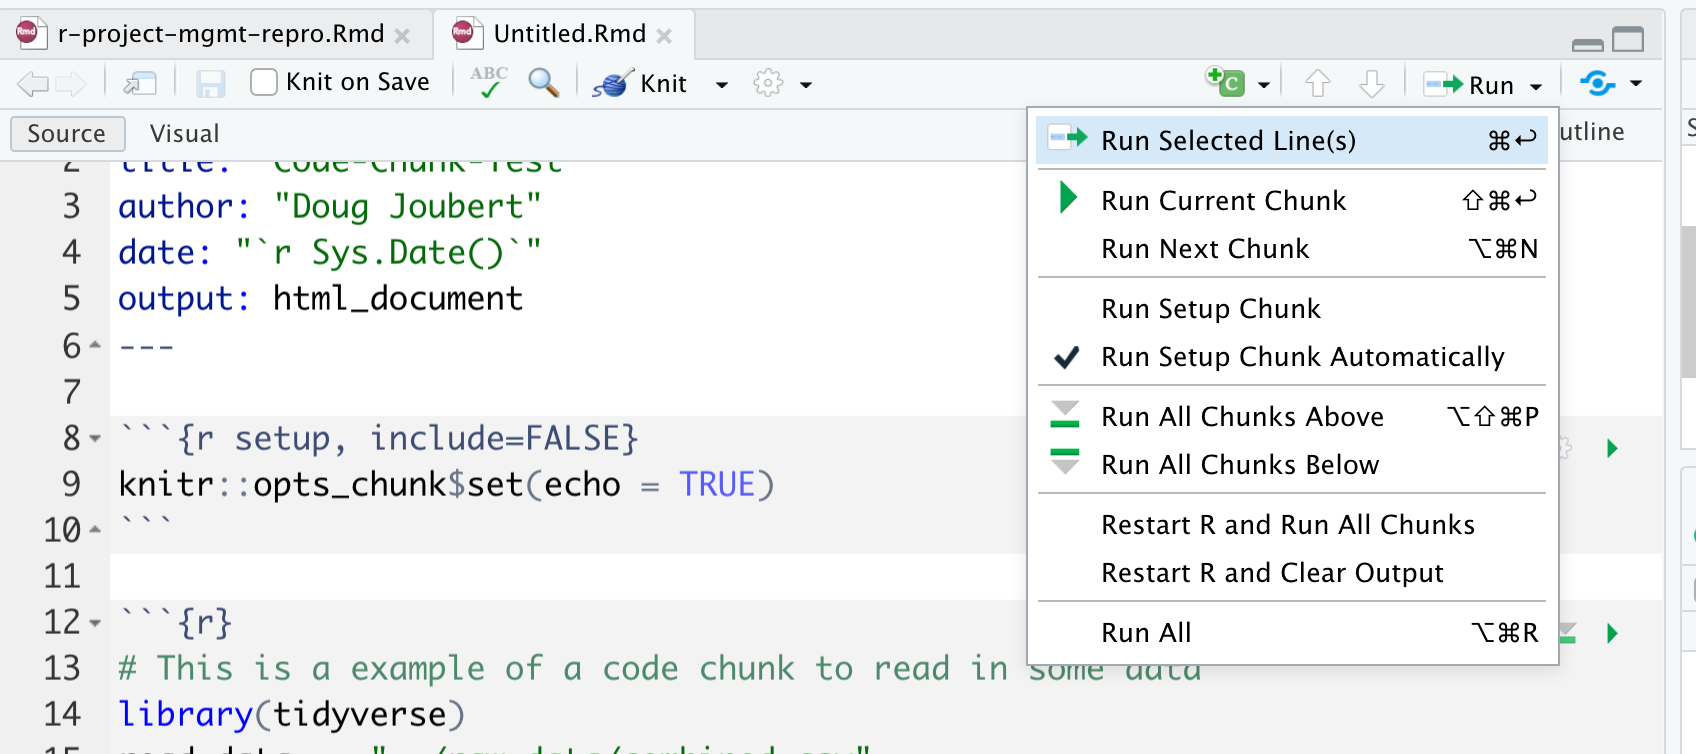
\includegraphics[width=6.5in,height=\textheight]{images/code-run-chunk-02.png}

Figure 14: Running a code chunk from the Code-Chunk menu.

\begin{enumerate}
\def\labelenumi{\arabic{enumi}.}
\setcounter{enumi}{2}
\tightlist
\item
  Using keyboard shortcuts
\end{enumerate}

\begin{longtable}[]{@{}
  >{\raggedright\arraybackslash}p{(\columnwidth - 4\tabcolsep) * \real{0.4000}}
  >{\raggedright\arraybackslash}p{(\columnwidth - 4\tabcolsep) * \real{0.3000}}
  >{\raggedright\arraybackslash}p{(\columnwidth - 4\tabcolsep) * \real{0.3000}}@{}}
\toprule
\begin{minipage}[b]{\linewidth}\raggedright
\textbf{Task}
\end{minipage} & \begin{minipage}[b]{\linewidth}\raggedright
\textbf{Windows \& Linux}
\end{minipage} & \begin{minipage}[b]{\linewidth}\raggedright
\textbf{macOS}
\end{minipage} \\
\midrule
\endhead
Create a code chunk & Ctrl + Alt + I & Cmd + Option + I \\
Run all chunks above & Ctrl+Alt+P & Command+Option+P \\
Run current chunk & Ctrl+Alt+C & Command+Option+C \\
Run current chunk & Ctrl+Shift+Enter & Command+Shift+Enter \\
Run next chunk & Ctrl+Alt+N & Command+Option+N \\
Run all chunks & Ctrl+Alt+R & Command+Option+R \\
Go to next chunk/title & Ctrl+PgDown & Command+PgDown \\
Go to previous chunk/title & Ctrl+PgUp & Command+PgUp \\
\bottomrule
\end{longtable}

\hypertarget{labeling-code-chunk}{%
\subsection{\texorpdfstring{\textbf{Labeling Code
Chunk}}{Labeling Code Chunk}}\label{labeling-code-chunk}}

While not necessary for running your code, it is good practice is to
give a name to each code chunk because it gives the chunk a unique
identifier which allows for more advanced options (such as
cross-referencing) to work with your rmd files later on:

\texttt{\{r\ chunk-name\}}

Some things to keep in mind

\begin{itemize}
\item
  The chunk name is the only value other than r in the code chunk
  options that doesn't require a tag (i.e.~\texttt{echo\ =} )
\item
  The chunk label has to be unique (i.e.you can't use the the same name
  for multiple chunks)
\end{itemize}

We'll see in a bit where this code chunk label comes in handy. But, for
now let's go back and give our first code chunk a name:

\begin{enumerate}
\def\labelenumi{\arabic{enumi}.}
\item
  \texttt{\{r\ Importing\ our\ Data\}}
\item
  Then, run the code-chunk
\end{enumerate}

Figure 15 is displaying the output of the code-chunk. Can you explain
what is happening in the console?

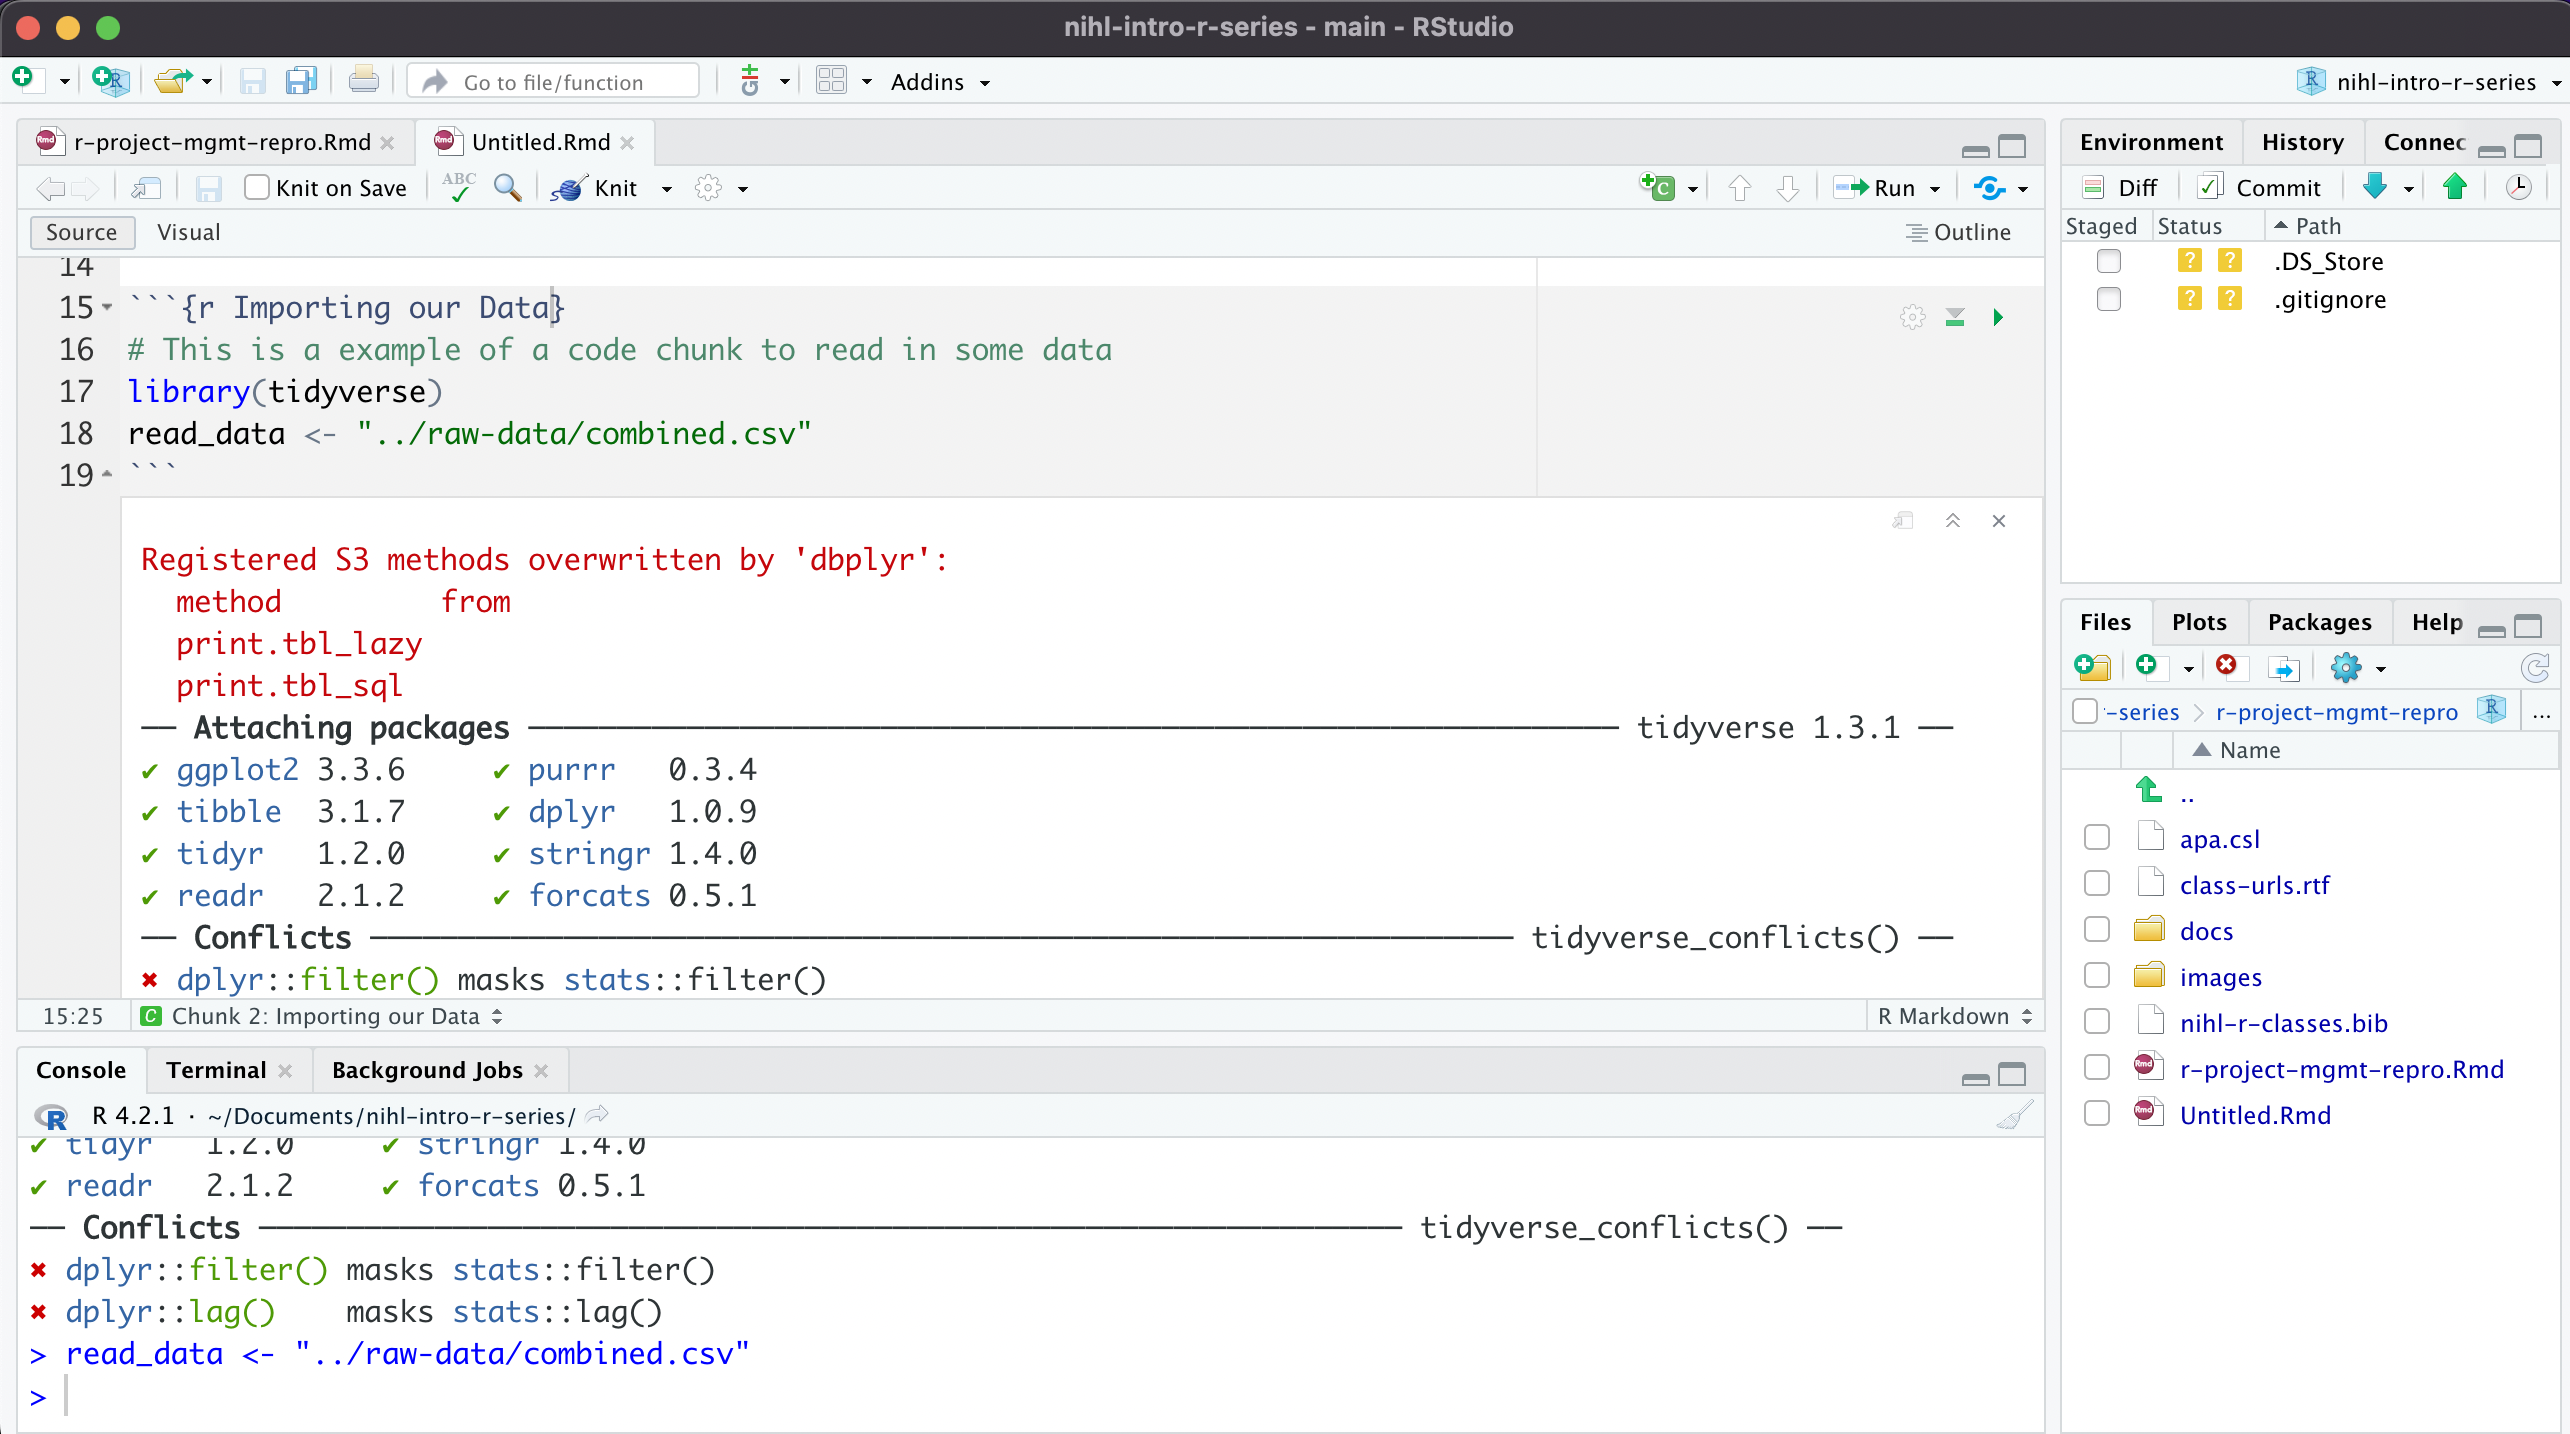
\includegraphics[width=6.5in,height=\textheight]{images/knit-02.png}

Figure 15: Output from our first code chunk.

\hypertarget{code-chunk-options}{%
\subsection{Code Chunk Options}\label{code-chunk-options}}

There are over 50 different code chunk options. Wow, that is a lot.
Obviously we will not go over all of them, but they fall into several
larger categories including: code evaluation, text output, code style,
cache options, plot output and animation.

You can find a complete list of code chunk options on Knitr developer,
Yihui Xie's, \href{https://yihui.org/knitr/options/}{online guide to
knitr}. Or, you can find a brief list of all options on the R Markdown
Reference guide on page 3 accesible through the RStudio Interface by
navigating to the main menu bar
\texttt{Help\ \textgreater{}\ Cheat\ Sheets\ \textgreater{}\ R\ Markdown\ Reference\ Guide}.

The chunk name is the only value other than \texttt{r} in the code chunk
options that doesn't require a tag (i.e.~the ``= VALUE'' part of
\texttt{option\ =\ VALUE}). So chunk options will always require a tag,
and the syntax will be in the form:

\texttt{\{r\ chunk-label,\ option\ =\ VALUE\}}

The option always follows the code chunk label (don't forget to add a
\texttt{,} after the label either).

\hypertarget{code-evaluation-option}{%
\subsection{Code Evaluation Option}\label{code-evaluation-option}}

\begin{itemize}
\tightlist
\item
  \textbf{include} = (logical) whether to include the chunk output in
  the output document (defaults to TRUE).
\end{itemize}

\hypertarget{text-output-options}{%
\subsection{\texorpdfstring{\textbf{Text Output
Options}}{Text Output Options}}\label{text-output-options}}

\begin{itemize}
\item
  \textbf{eval} = (logical or numeric) TRUE/FALSE to evaluate (or not)
  or a numeric value like c(1,3) (only evaluate expressions 1 and 3)
\item
  \textbf{echo} = (logical or numeric - following the same rules as
  above) whether to display source code or not.
\item
  \textbf{results} = (logical or character) text output of the code can
  be hidden (hide or FALSE), or delineated in a certain way (default
  `markup').
\item
  \textbf{warning} = (logical) whether to display the warnings in the
  output (default TRUE). FALSE will output warnings to the console only.
\item
  \textbf{message} = (logical) whether or not to display messages that
  appear when running the code (default TRUE).
\end{itemize}

\hypertarget{producing-your-document}{%
\subsection{Producing Your Document}\label{producing-your-document}}

\hypertarget{knitr}{%
\subsection{Knitr}\label{knitr}}

\href{https://yihui.org/knitr/}{Knitr} is the engine in RStudio which
creates the ``dynamic'' part of R Markdown reports. It's specifically a
package that allows the integration of R code into the html, word, pdf,
or LaTex document you have specified as your output for R Markdown.

We just saw how to run our code in our code chunks to see a preview of
the code output. However, if we want to produce a final report with
code, we need to use the Knit button. Using the knit button with code
chunks is a two step process:

\begin{enumerate}
\def\labelenumi{\arabic{enumi}.}
\tightlist
\item
  The code is run (all code chunks will run automatically).
\item
  Second, (if there are no code errors) the document of choice will
  render for our whole R Markdown document.
\item
  Figure 15 is showing the Knitr options available
\end{enumerate}

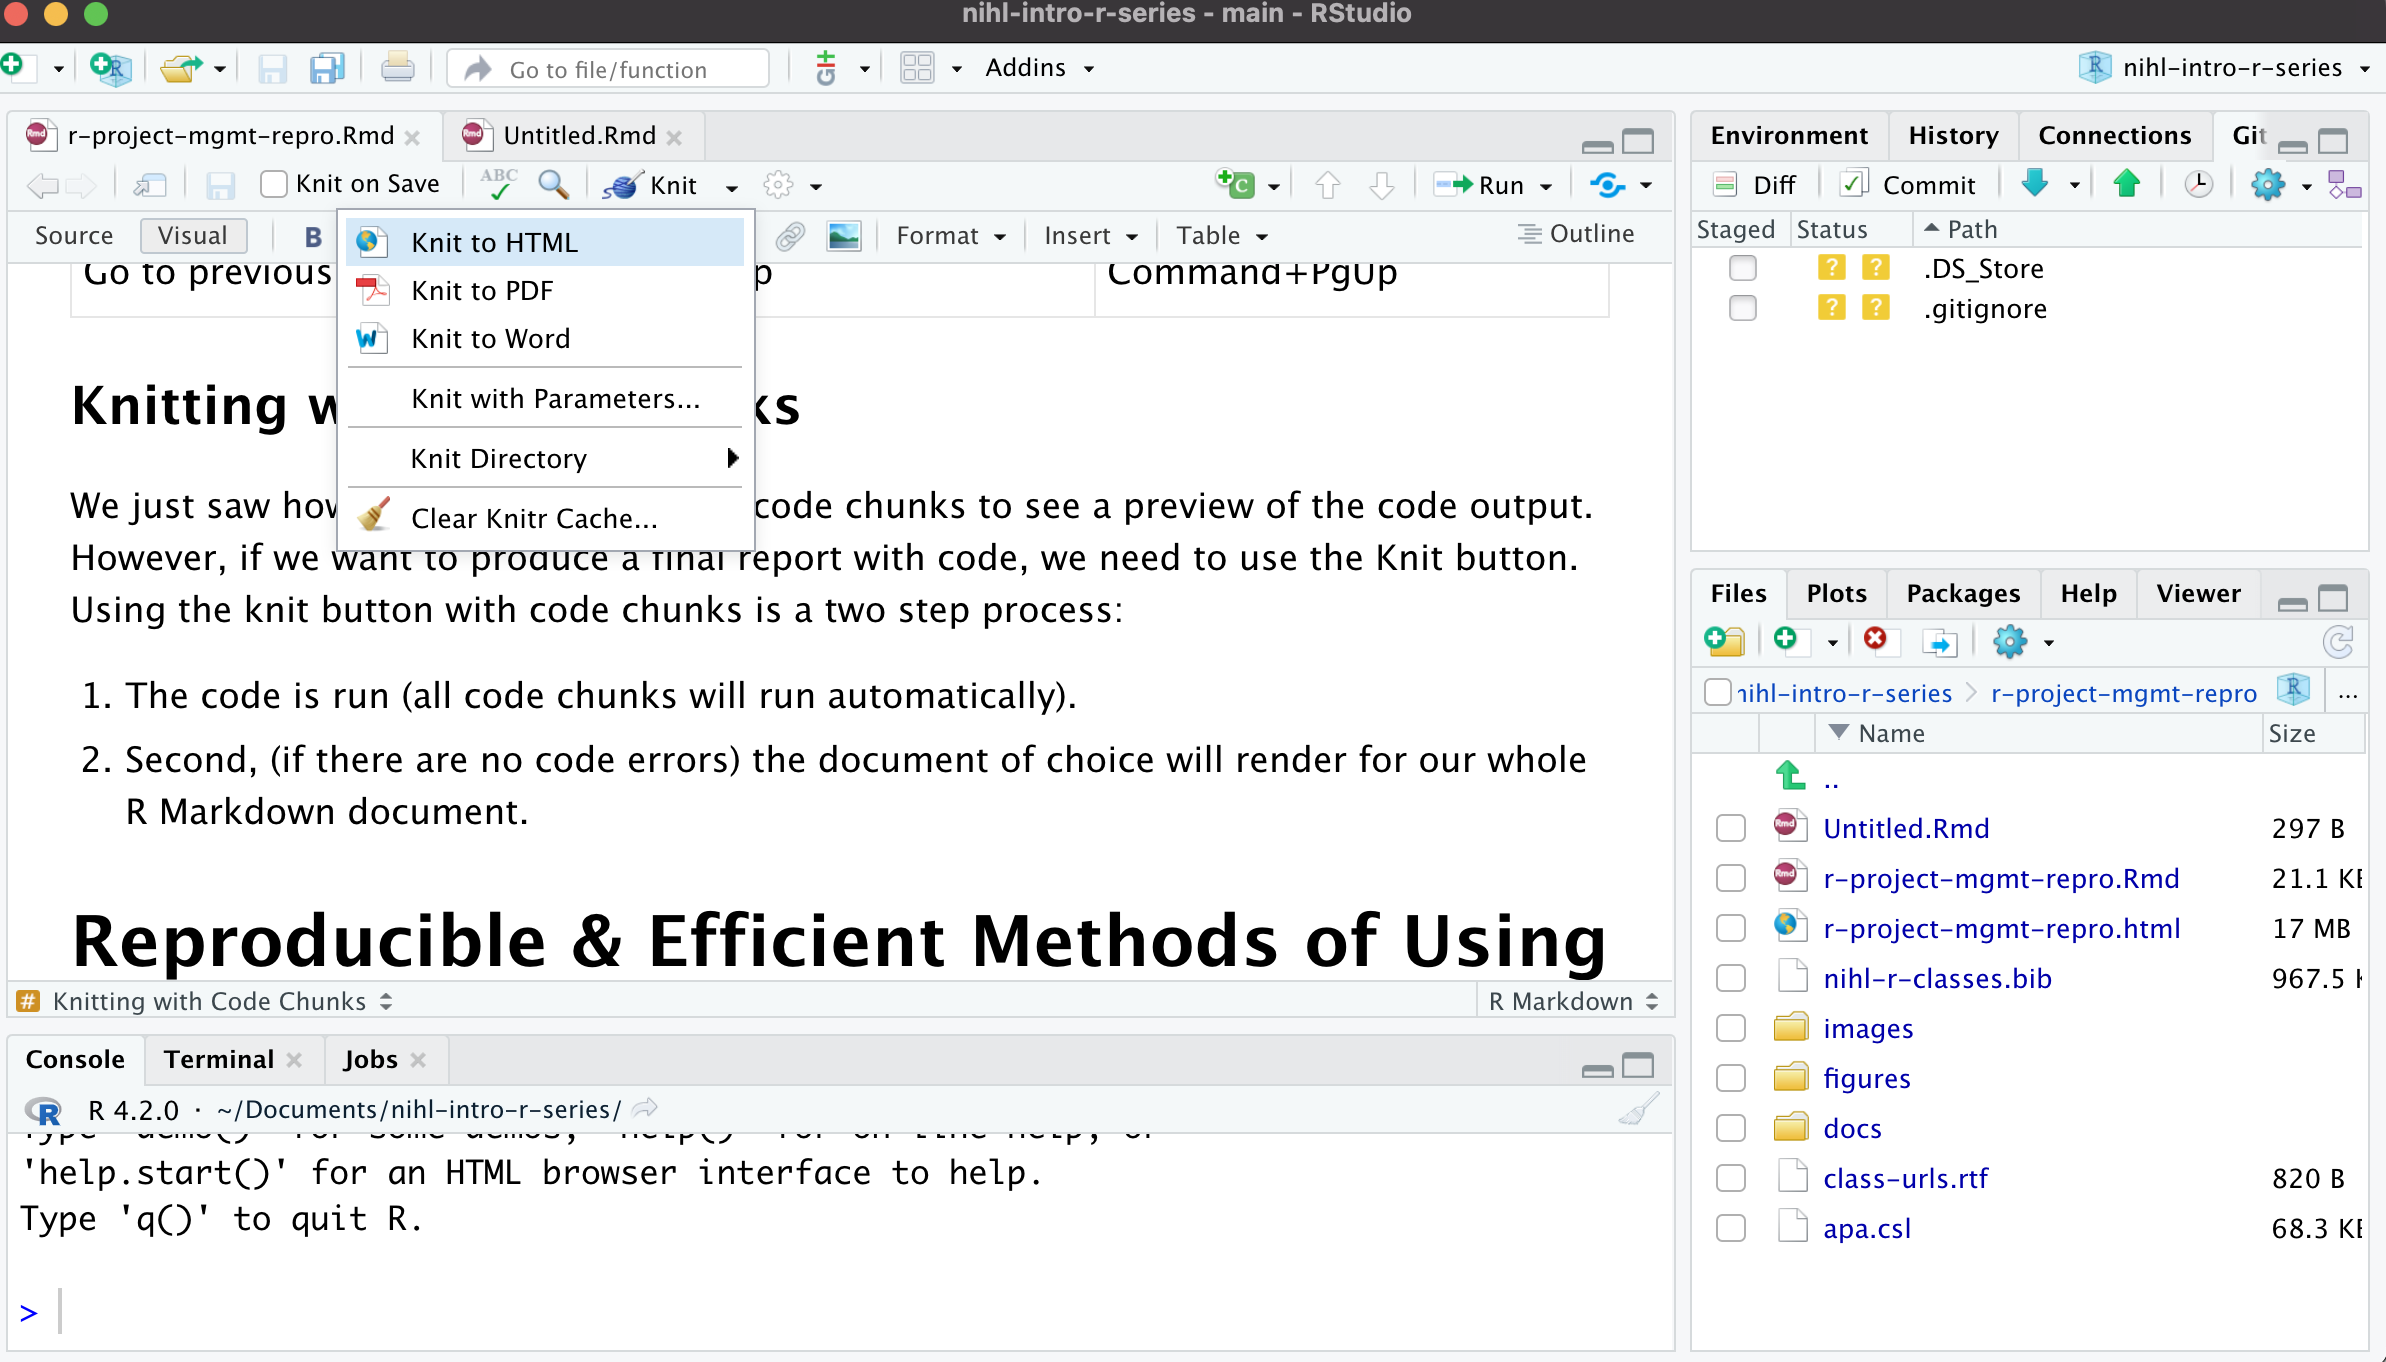
\includegraphics[width=6.5in,height=\textheight]{images/knit-01.png}

Figure 15: Knitr options in R-markdown.

\hypertarget{global-code-chunk-options}{%
\section{\texorpdfstring{\textbf{Global Code Chunk
Options}}{Global Code Chunk Options}}\label{global-code-chunk-options}}

Let's direct our attention back to the first code chunk in this document
that I asked you not to delete.

The code looks like:

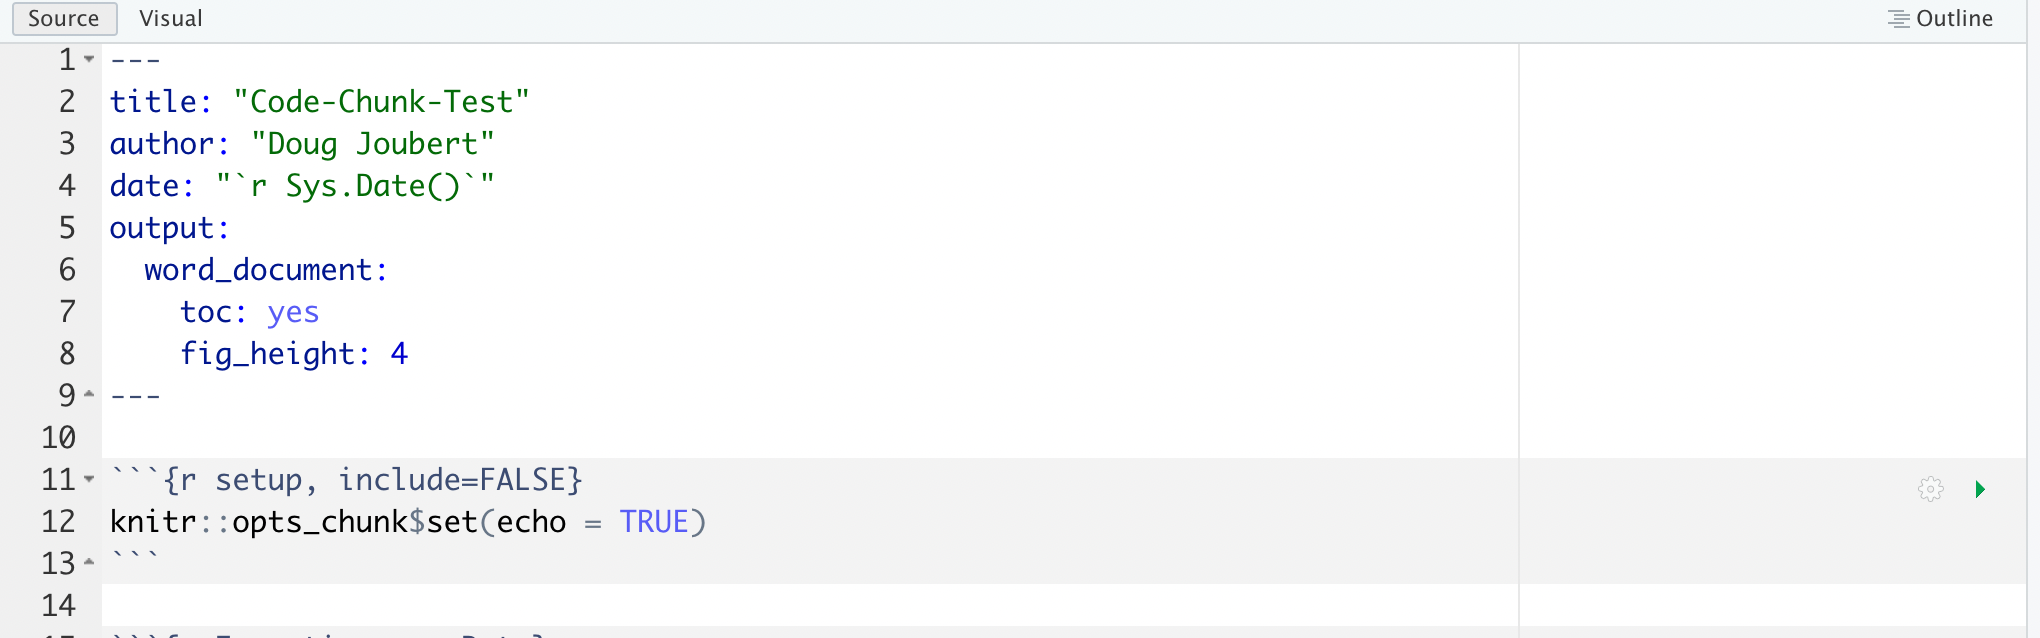
\includegraphics[width=6.5in,height=\textheight]{images/code-chunk-03.png}

Figure 16: Example of a global code chunk.

This is an option to globally set options for the entire R Markdown
document. Can you imagine how much work it would be to add the chunk
options each time? Also, what if we need different options for different
figures. We can automate setting options by adding this special code
chunk at the beginning of the document. Then, each code chunk we add
will refer to those ``global'' options when it runs.

\hypertarget{reproducible-efficient-methods-of-using-code-chunks}{%
\section{Reproducible \& Efficient Methods of Using Code
Chunks}\label{reproducible-efficient-methods-of-using-code-chunks}}

I think this should be an advanced class. I will need to identify
``breakpoints'' after I do the dry run and teach the class for the first
time.

\hypertarget{bibliography-citations-cross-referencing}{%
\section{Bibliography, Citations \&
Cross-Referencing}\label{bibliography-citations-cross-referencing}}

Older versions of RStudio require
\href{https://pandoc.org/MANUAL.html\#citation-syntax}{Pandoc's}
citation syntax to render bibliographies correctly. We won't be covering
this approach extensively in this workshop, since the new visual editor
has made this process much more simple. You can refer to our
\href{https://ucsbcarpentry.github.io/R-markdown/06-citations-bib/index.html}{previous
workshop on R Markdown} pre-visual editor for more information.

The new visual editor in RStudio 1.4 has made citations and
cross-referencing much easier, by offering different options for
referencing various types of sources. Before getting into these
different features, let's first learn how you can call the citation
window dialog on Rstudio and how to navigate these different options.

\hypertarget{creating-your-reference-list}{%
\subsection{Creating Your Reference
List}\label{creating-your-reference-list}}

You need to have a list of references saved to a bib file before you can
insert citations into your R-markdown document. A file with the BIB file
extension is a BibTeX Bibliographical Database file. It's a specially
formatted text file that lists references pertaining to a particular
source of information. Each item can be edited, in case there is any
metadata incorrect or missing.

There are a number of ways to create your bib file.

\begin{enumerate}
\def\labelenumi{\arabic{enumi}.}
\tightlist
\item
  Manually
\item
  Use a citation tool like Endnote or Zotero
\item
  Use the lookup feature to search for publications by DOI (Digital
  Object Identifier), Crossref, DataCite, or PubMed ID
\end{enumerate}

Most citation and reference management tools such as Refworks, Endnote,
Mendeley and Zotero, as well as some most scientific databases allow you
to export citations as .bib
\href{https://en.wikipedia.org/wiki/BibTeX}{BibteX} files.. I am going
to show you how to export references from Endnote to your bib file.
Figure 17 is displaying all of the references in my Endnote Library. I
have highlighted the Bioinformatics folder since I only want to explore
these records.

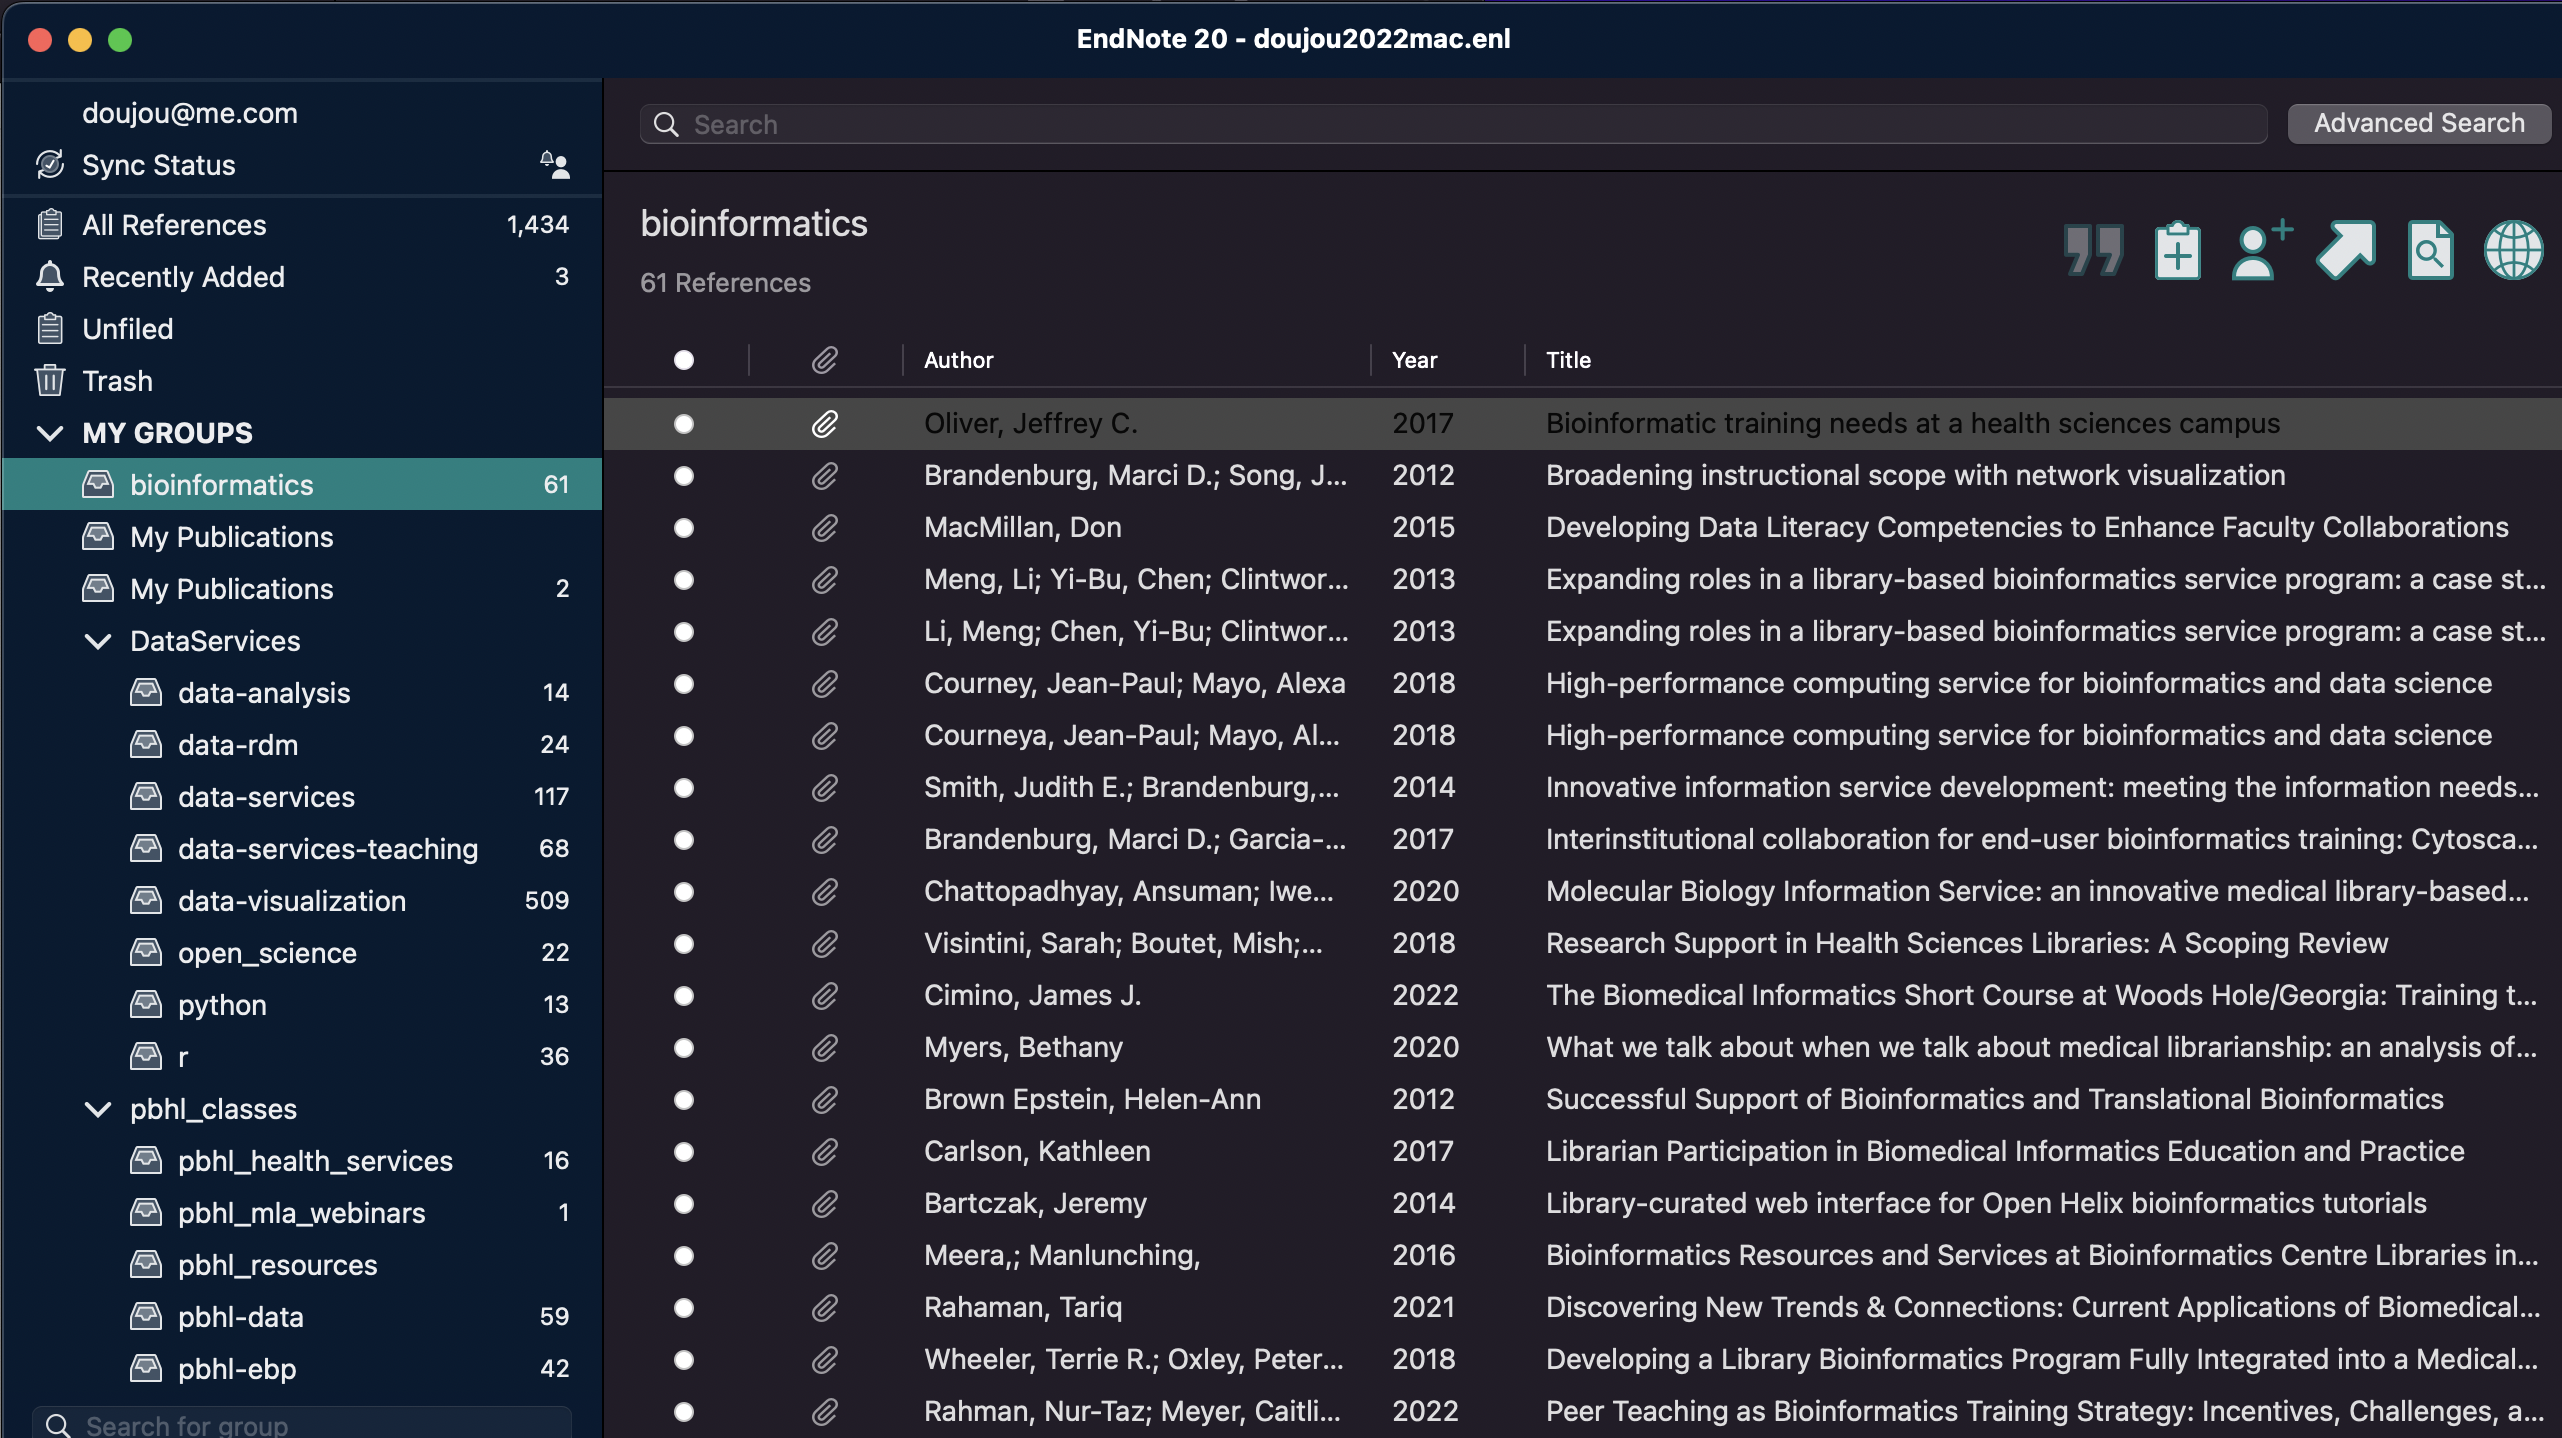
\includegraphics[width=6.66667in,height=\textheight]{images/bib-01.png}

Figure 17: Example of an Endnote Library.

The first thing I need to do is to get the records in the correct format
(bibtex). The Output Style Manager is locating under the Tools Menu (I
am on Mac OS) {[}Figure 18{]}.

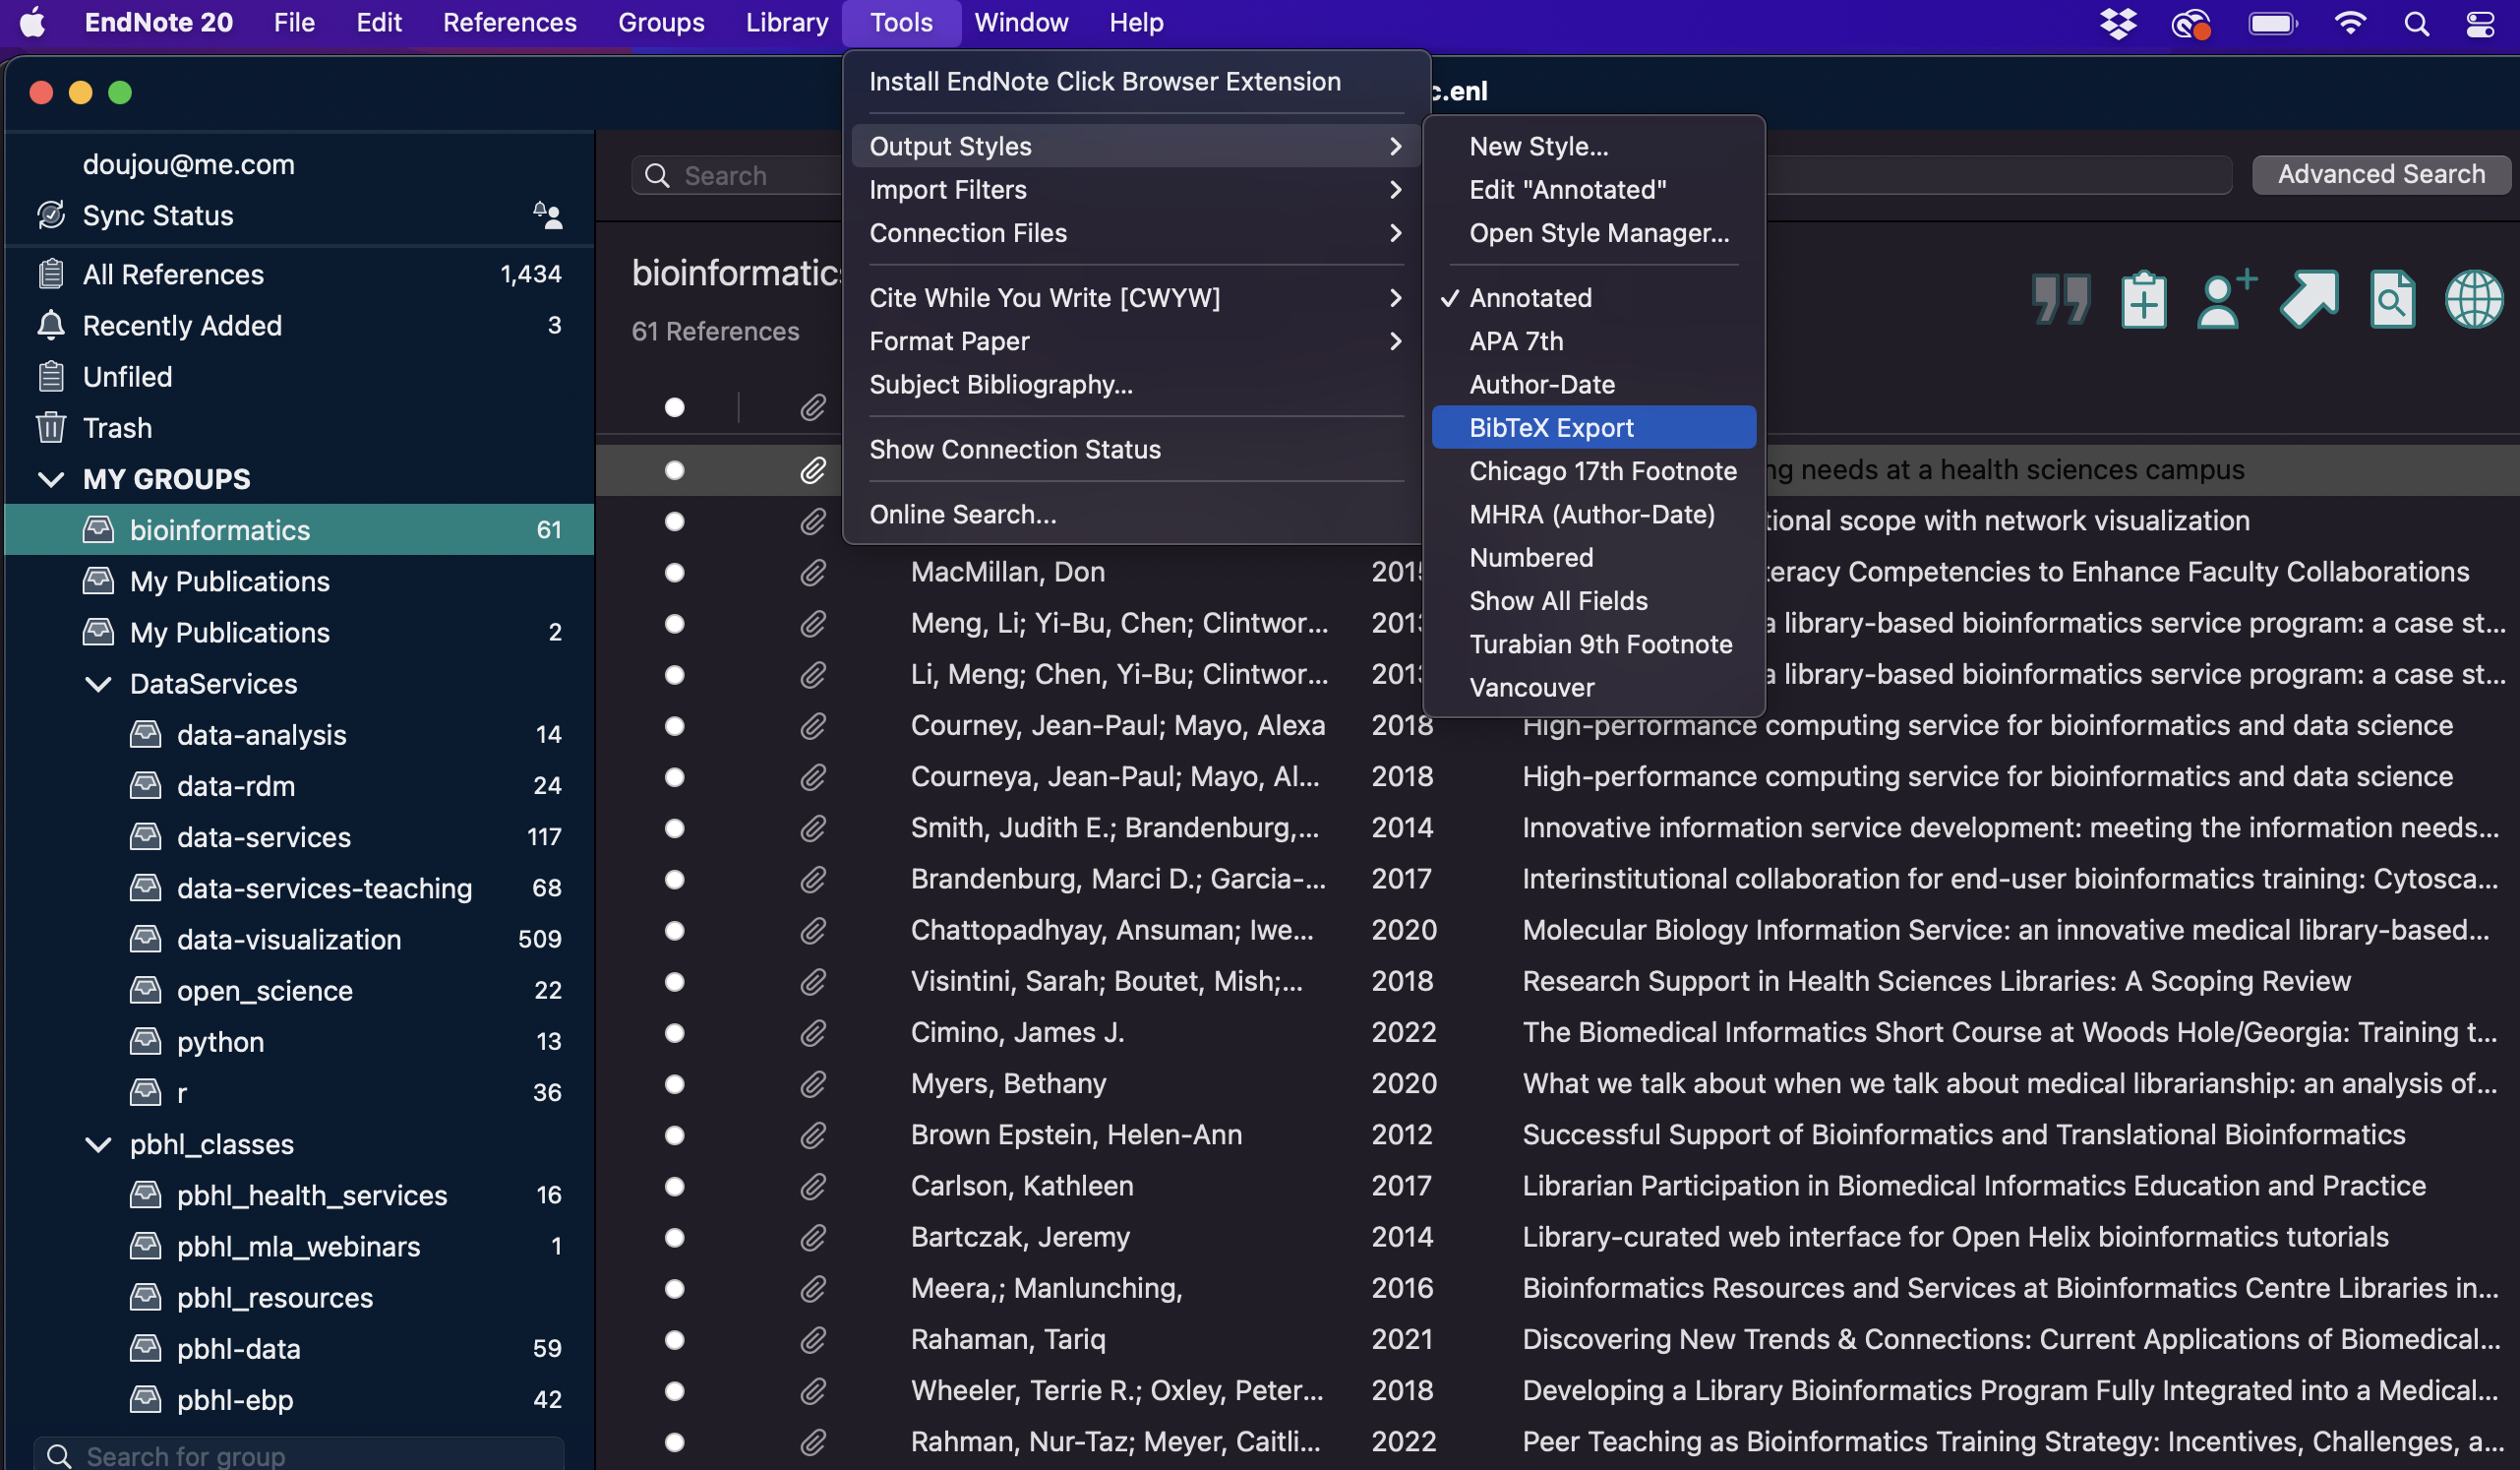
\includegraphics[width=6.5in,height=\textheight]{images/bib-02.png}

Figure 18: Selecting the bibtext output format in Endnote.

If \emph{bibtext} format is not in the list of styles, you can use
\textbf{Open Style Manager} to search for the \emph{bibtex} format.

The next step is to select all of the references that you want in your
bib file and choose the \textbf{Copy Formatted Reference} option
{[}Figure 19{]}. Please note that using \textbf{Copy} will not work.

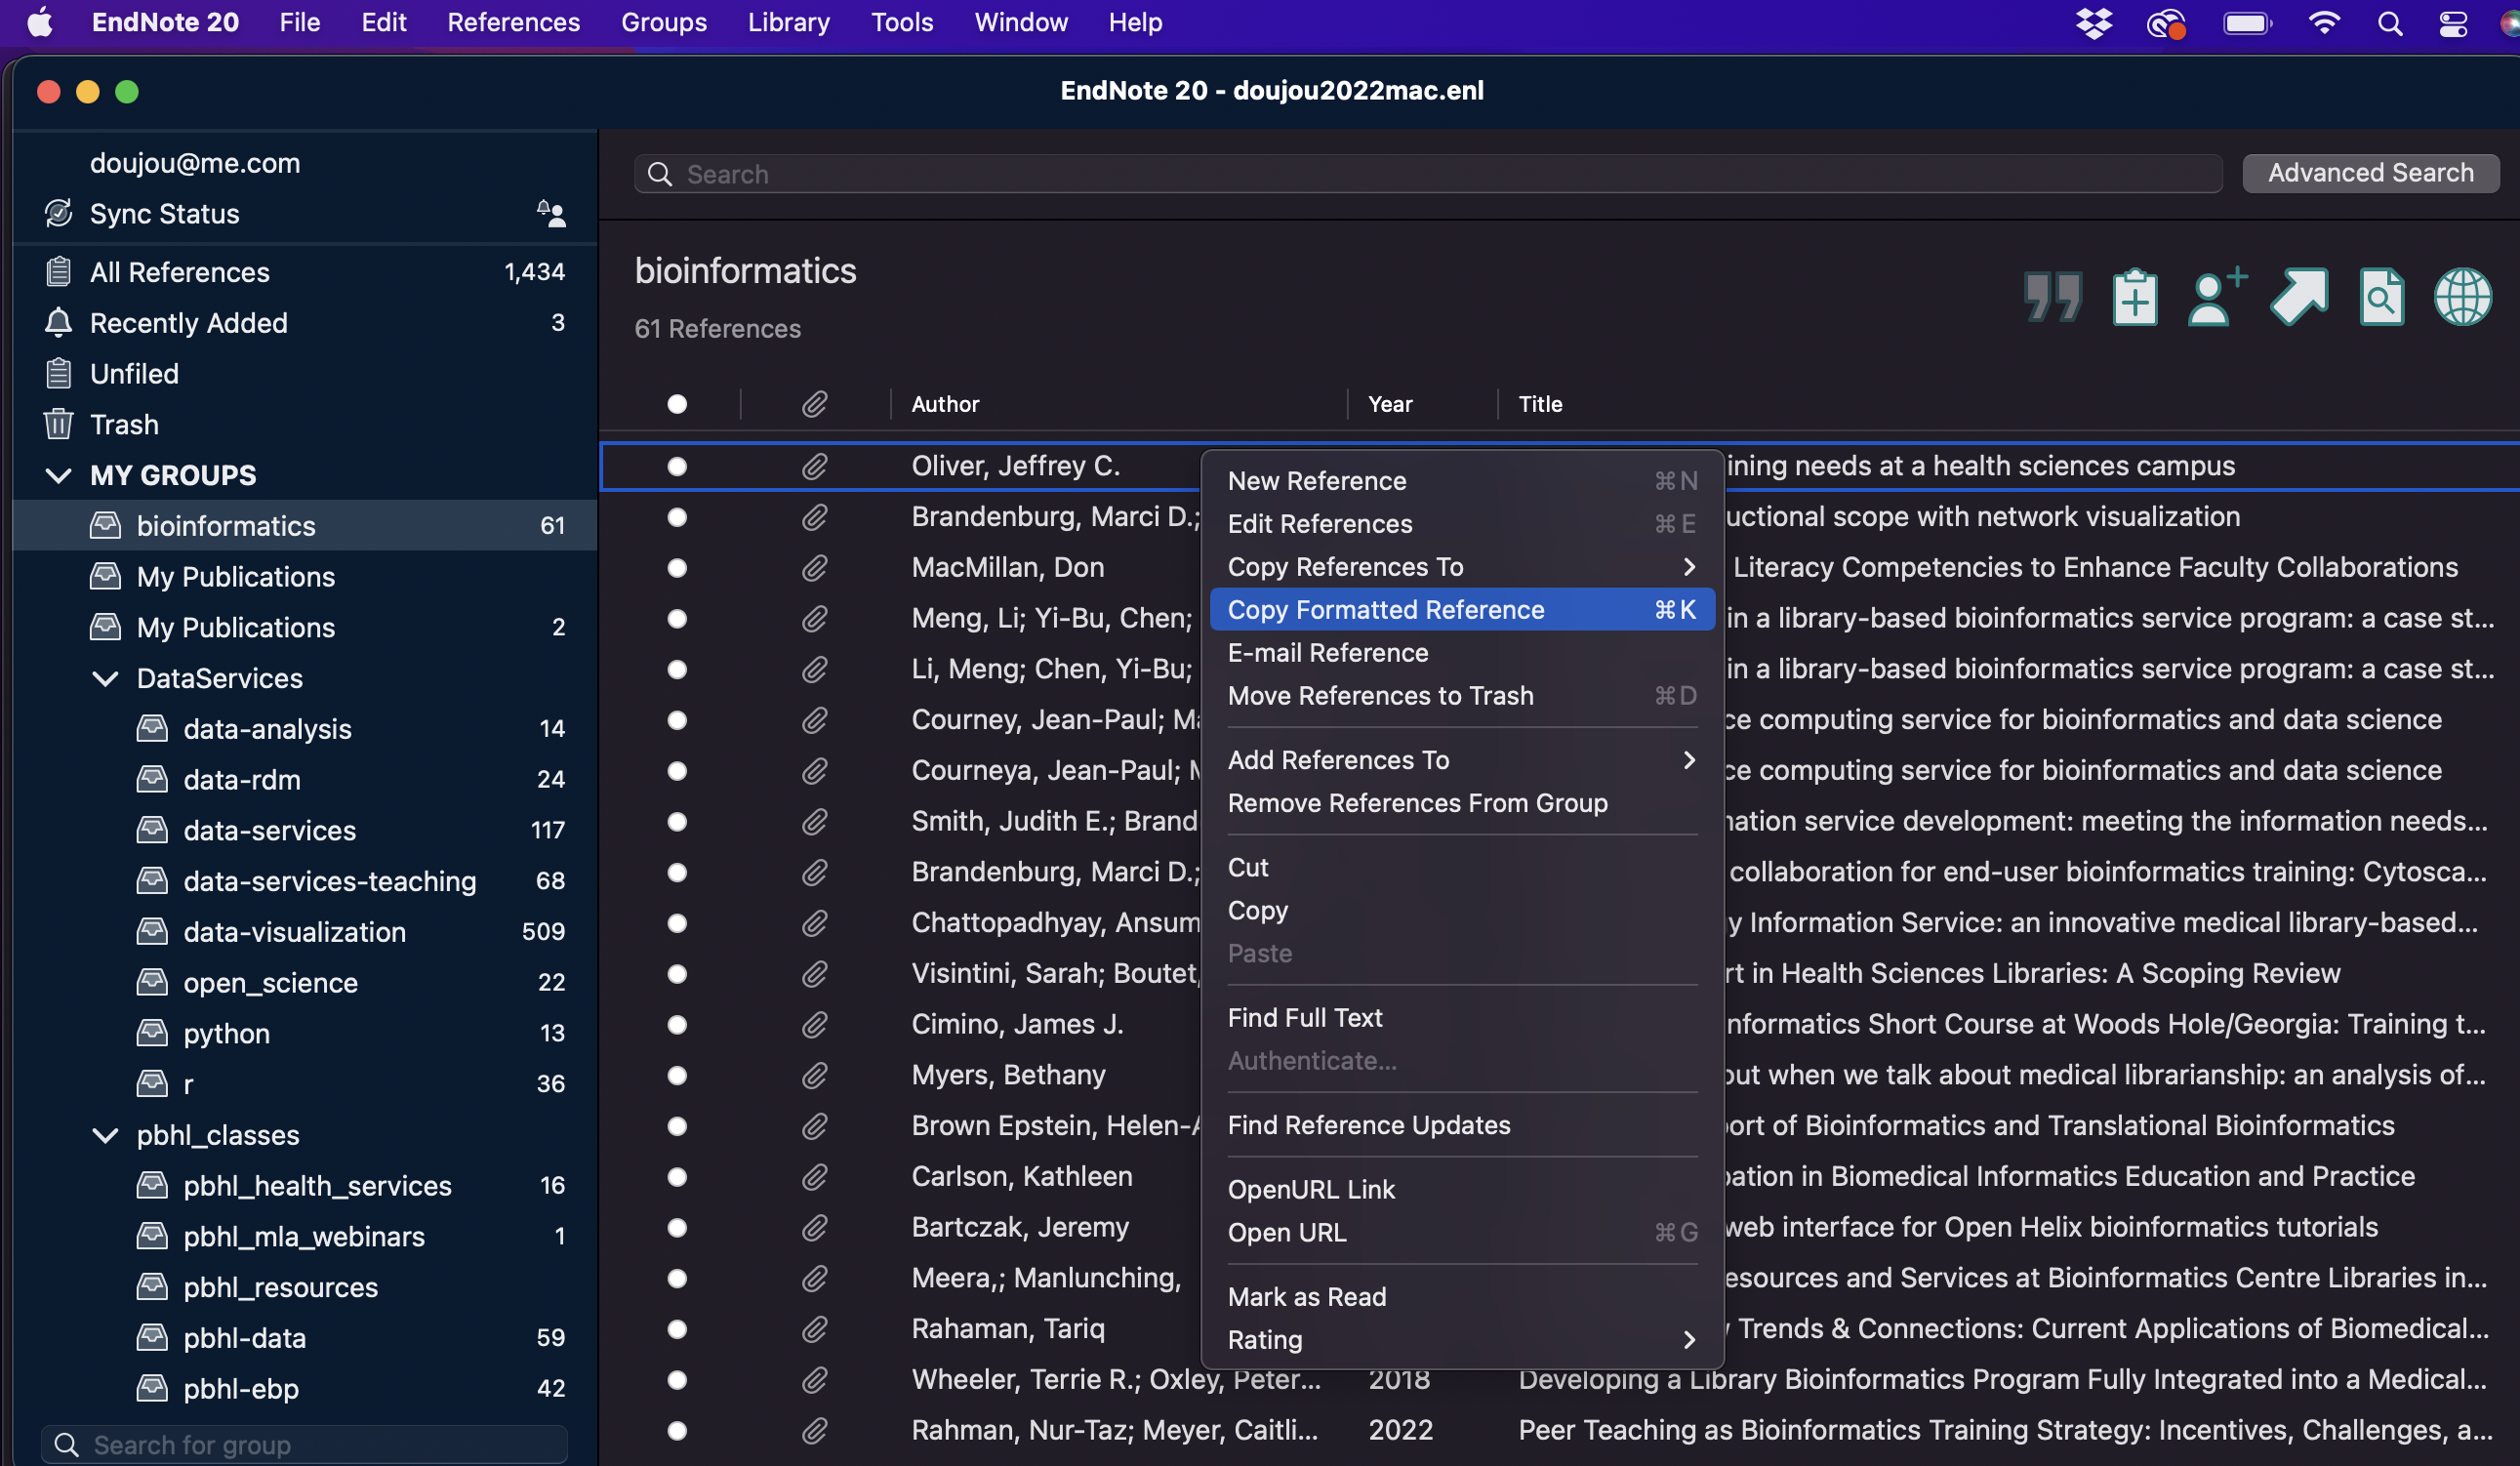
\includegraphics[width=6.6875in,height=\textheight]{images/bib-03.png}

Figure 19: Copying references from an Endnote Library in \emph{bibtext}
format.

Figure 20 i showing single reference that I pasted into a text editor.
As you can see in Figure 20, the \emph{bibtext} format is a tagged
format that starts with an \emph{article tag}.

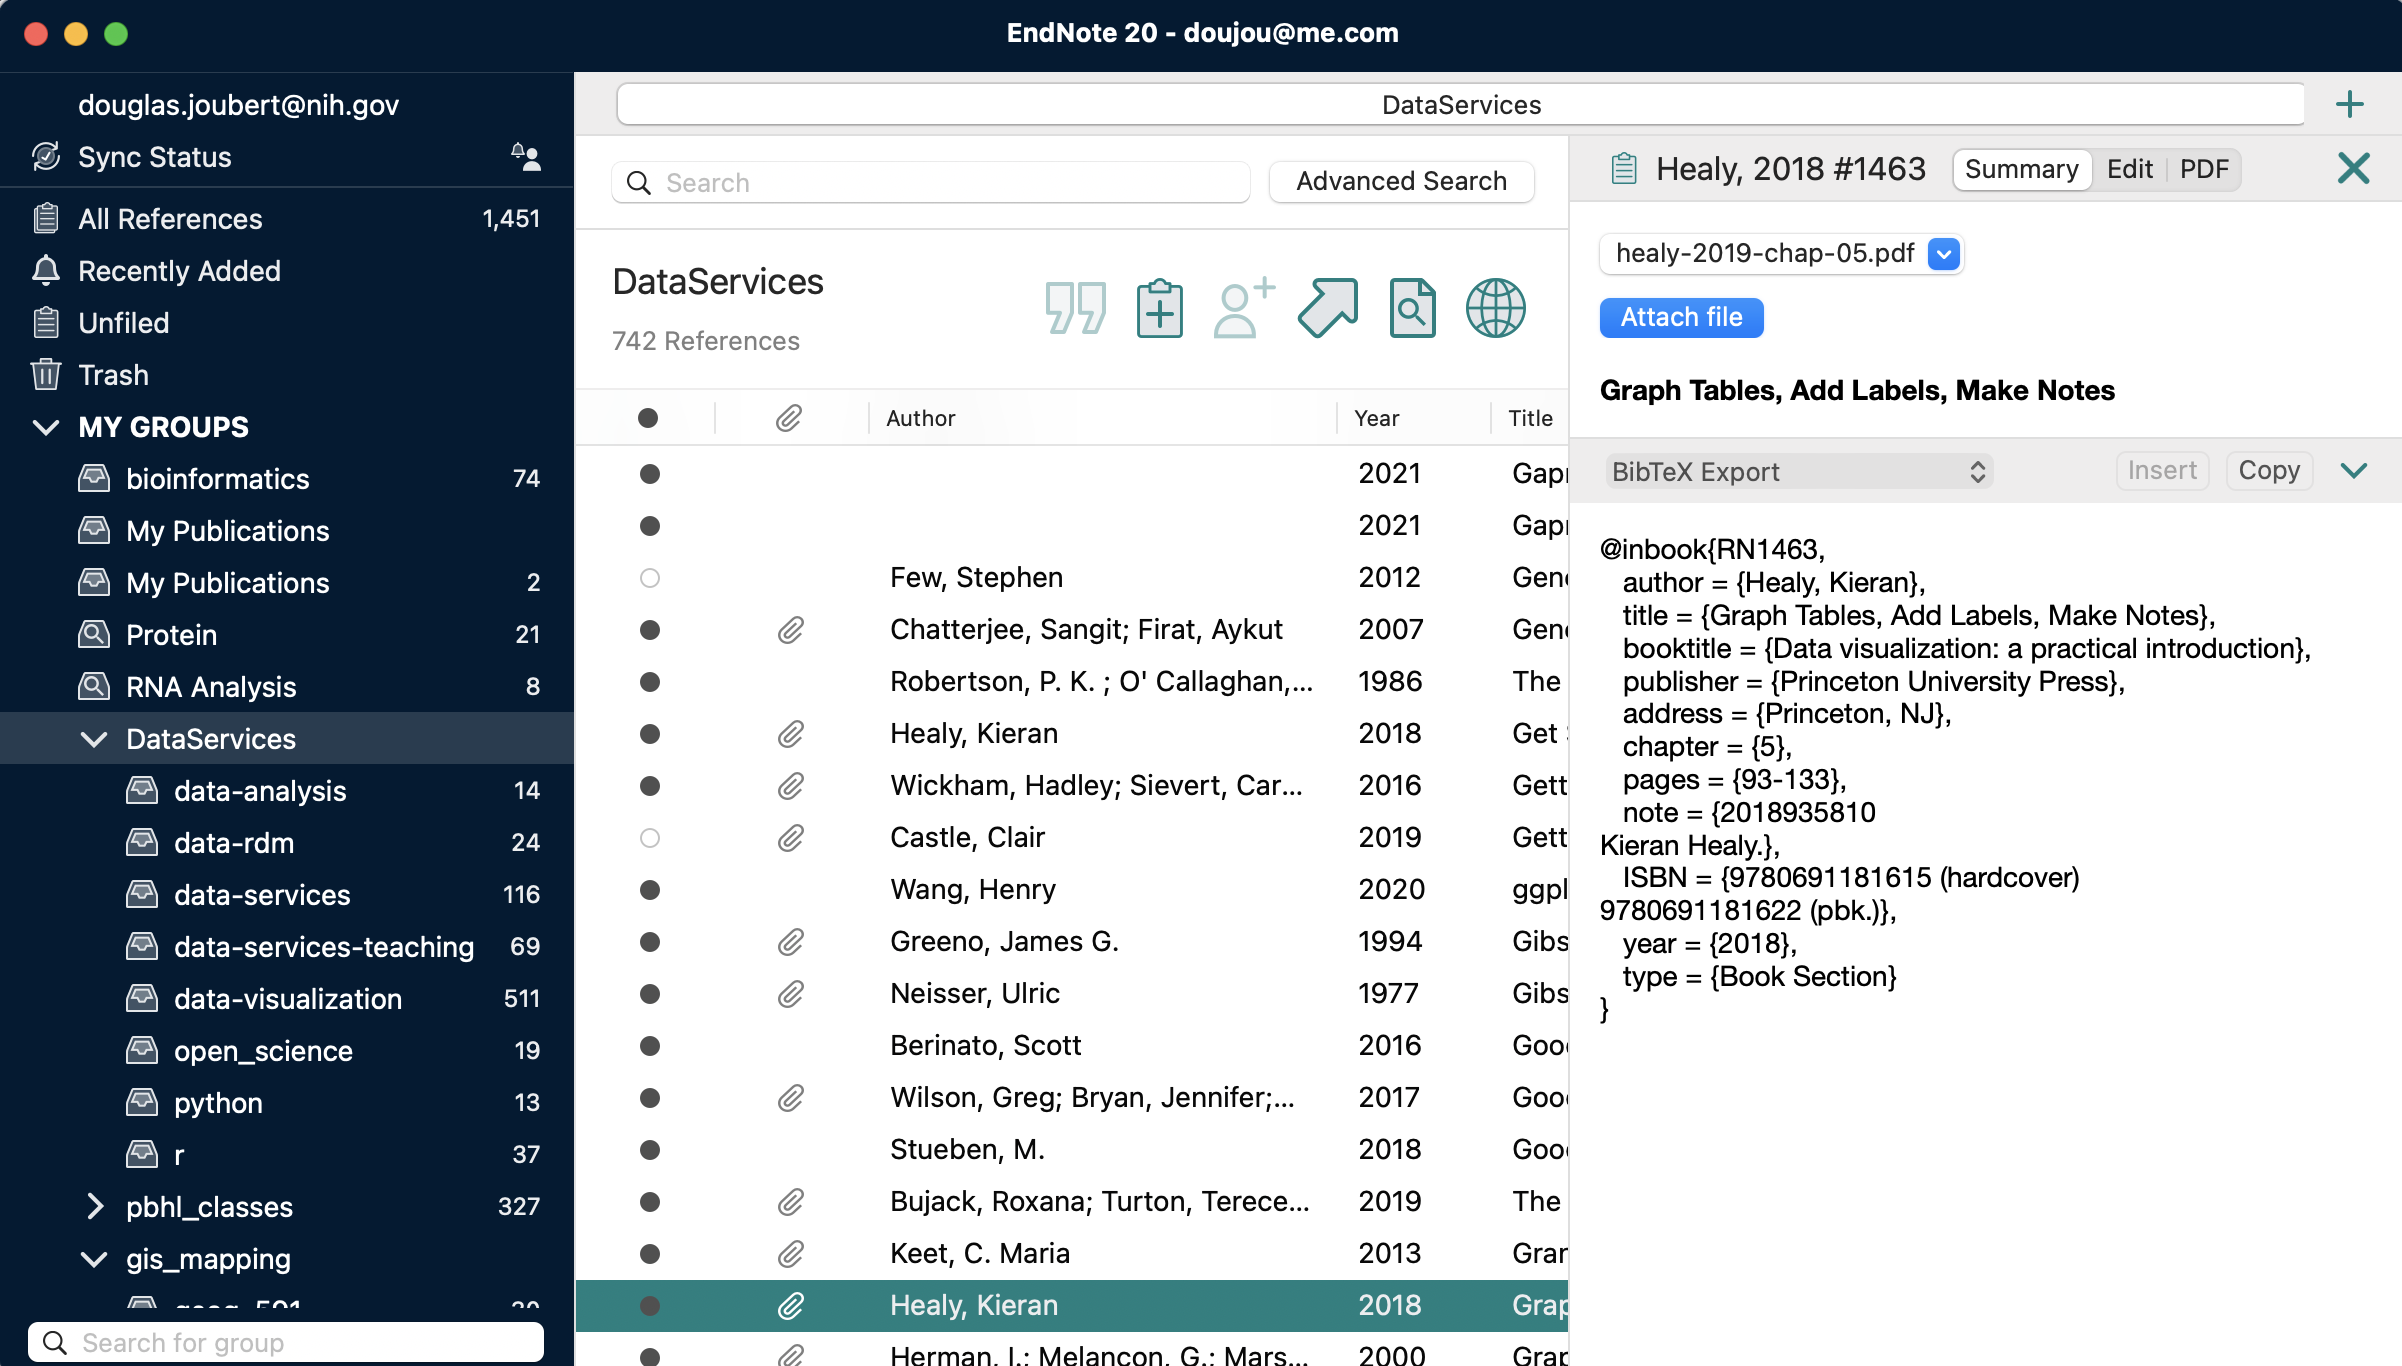
\includegraphics[width=6.66667in,height=\textheight]{images/bib-04.png}

Figure 20: Example of a record in bibtext format.

The BibTeX \href{http://www.bibtex.org/Format/}{website} is a great
resources for learning more about formatting options. Overleaf is
another great
\href{Bibliography\%20management\%20with\%20bibtex}{resource} with a
focus on bibliographic management.

\hypertarget{saving-your-reference-list}{%
\subsection{Saving Your Reference
List}\label{saving-your-reference-list}}

There are two ways to export the selected references from Endnote:

\begin{enumerate}
\def\labelenumi{\arabic{enumi}.}
\tightlist
\item
  Copy and past into a text document
\item
  Using the Export feature in Endnote
\end{enumerate}

I will cover using the Export feature from Endnote. These steps are very
similar in Zotero, Refworks or Mendeley {[}Figure 21{]}:

\begin{enumerate}
\def\labelenumi{\arabic{enumi}.}
\tightlist
\item
  Make sure you have selected your records
\item
  Choose File-\textgreater Export in Endnote
\item
  Make sure the Output Style says BibTeX
\item
  Make sure the file extension is bib
\item
  Make sure you are saving the file in the same folder as your RMD file.
\item
  Click Save
\item
  Make sure the file was saved to the correct directory. Note, that you
  might have to manually check the file extensions after you export it.
\end{enumerate}

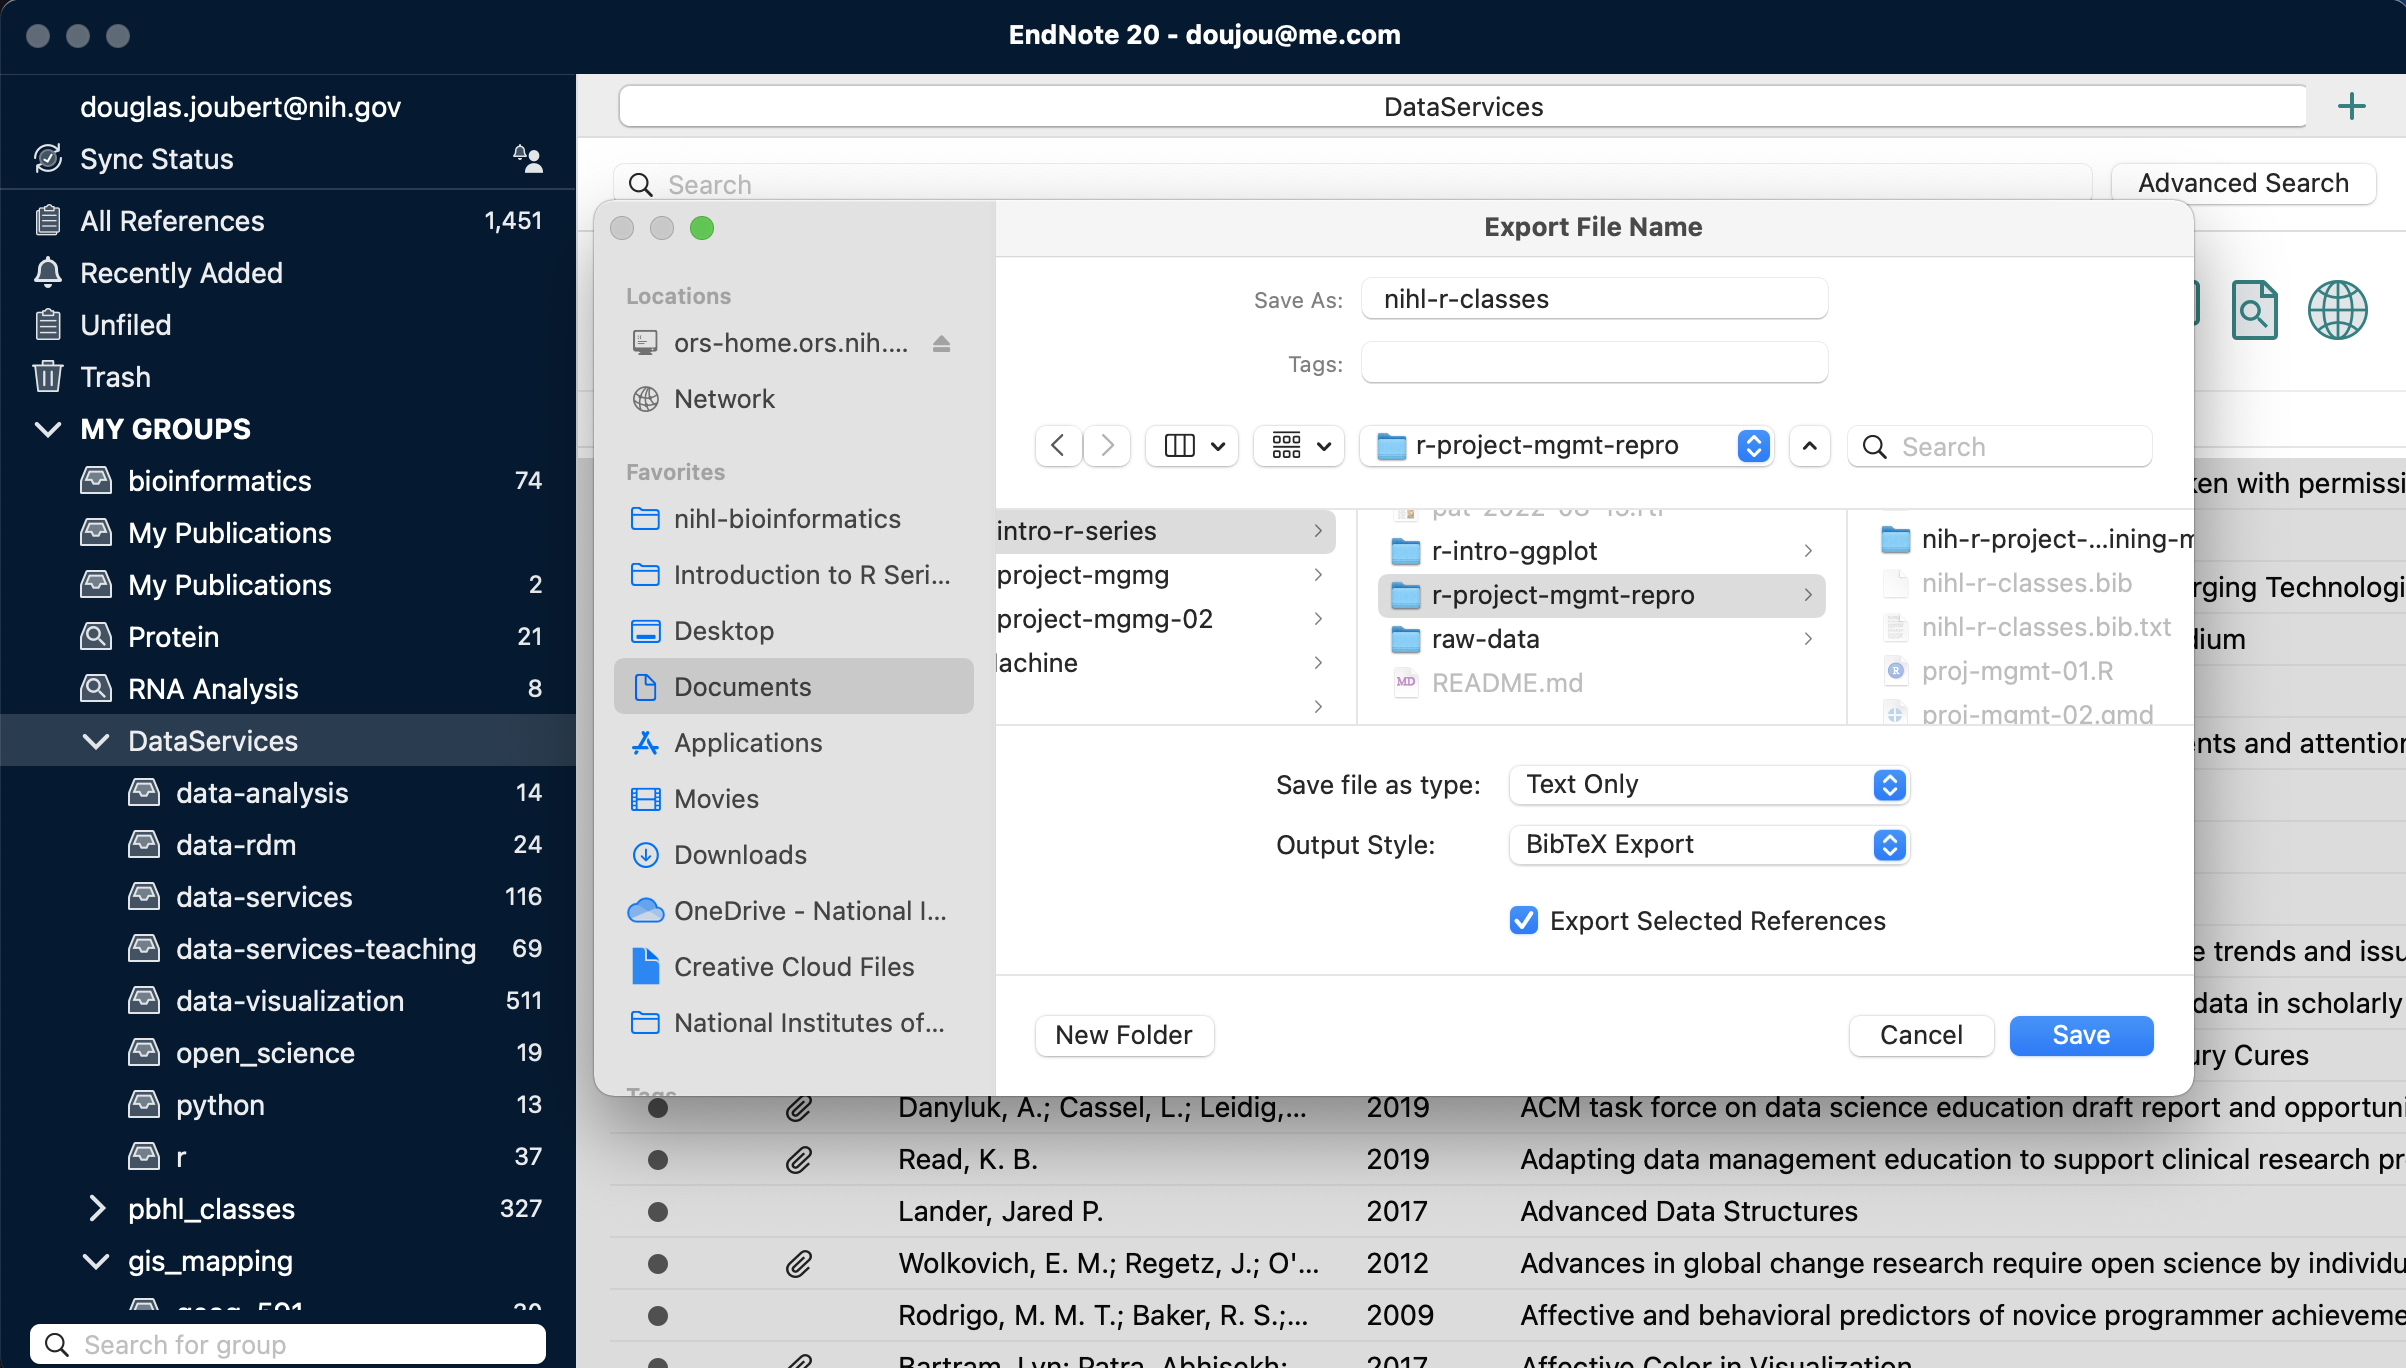
\includegraphics[width=6.66667in,height=\textheight]{images/bib-05.png}

Figure 21: Using the Export feature in Endnote.

\hypertarget{linking-the-bib-file-to-your-rmd-file}{%
\subsection{Linking the Bib File to Your RMD
file}\label{linking-the-bib-file-to-your-rmd-file}}

You must link the bib file and any associated output styles in the
Header of your RMD file. You need to add the following lines of code in
the Header {[}Figure 22{]}.

\texttt{bibliography:\ nihl-r-classes.bib}

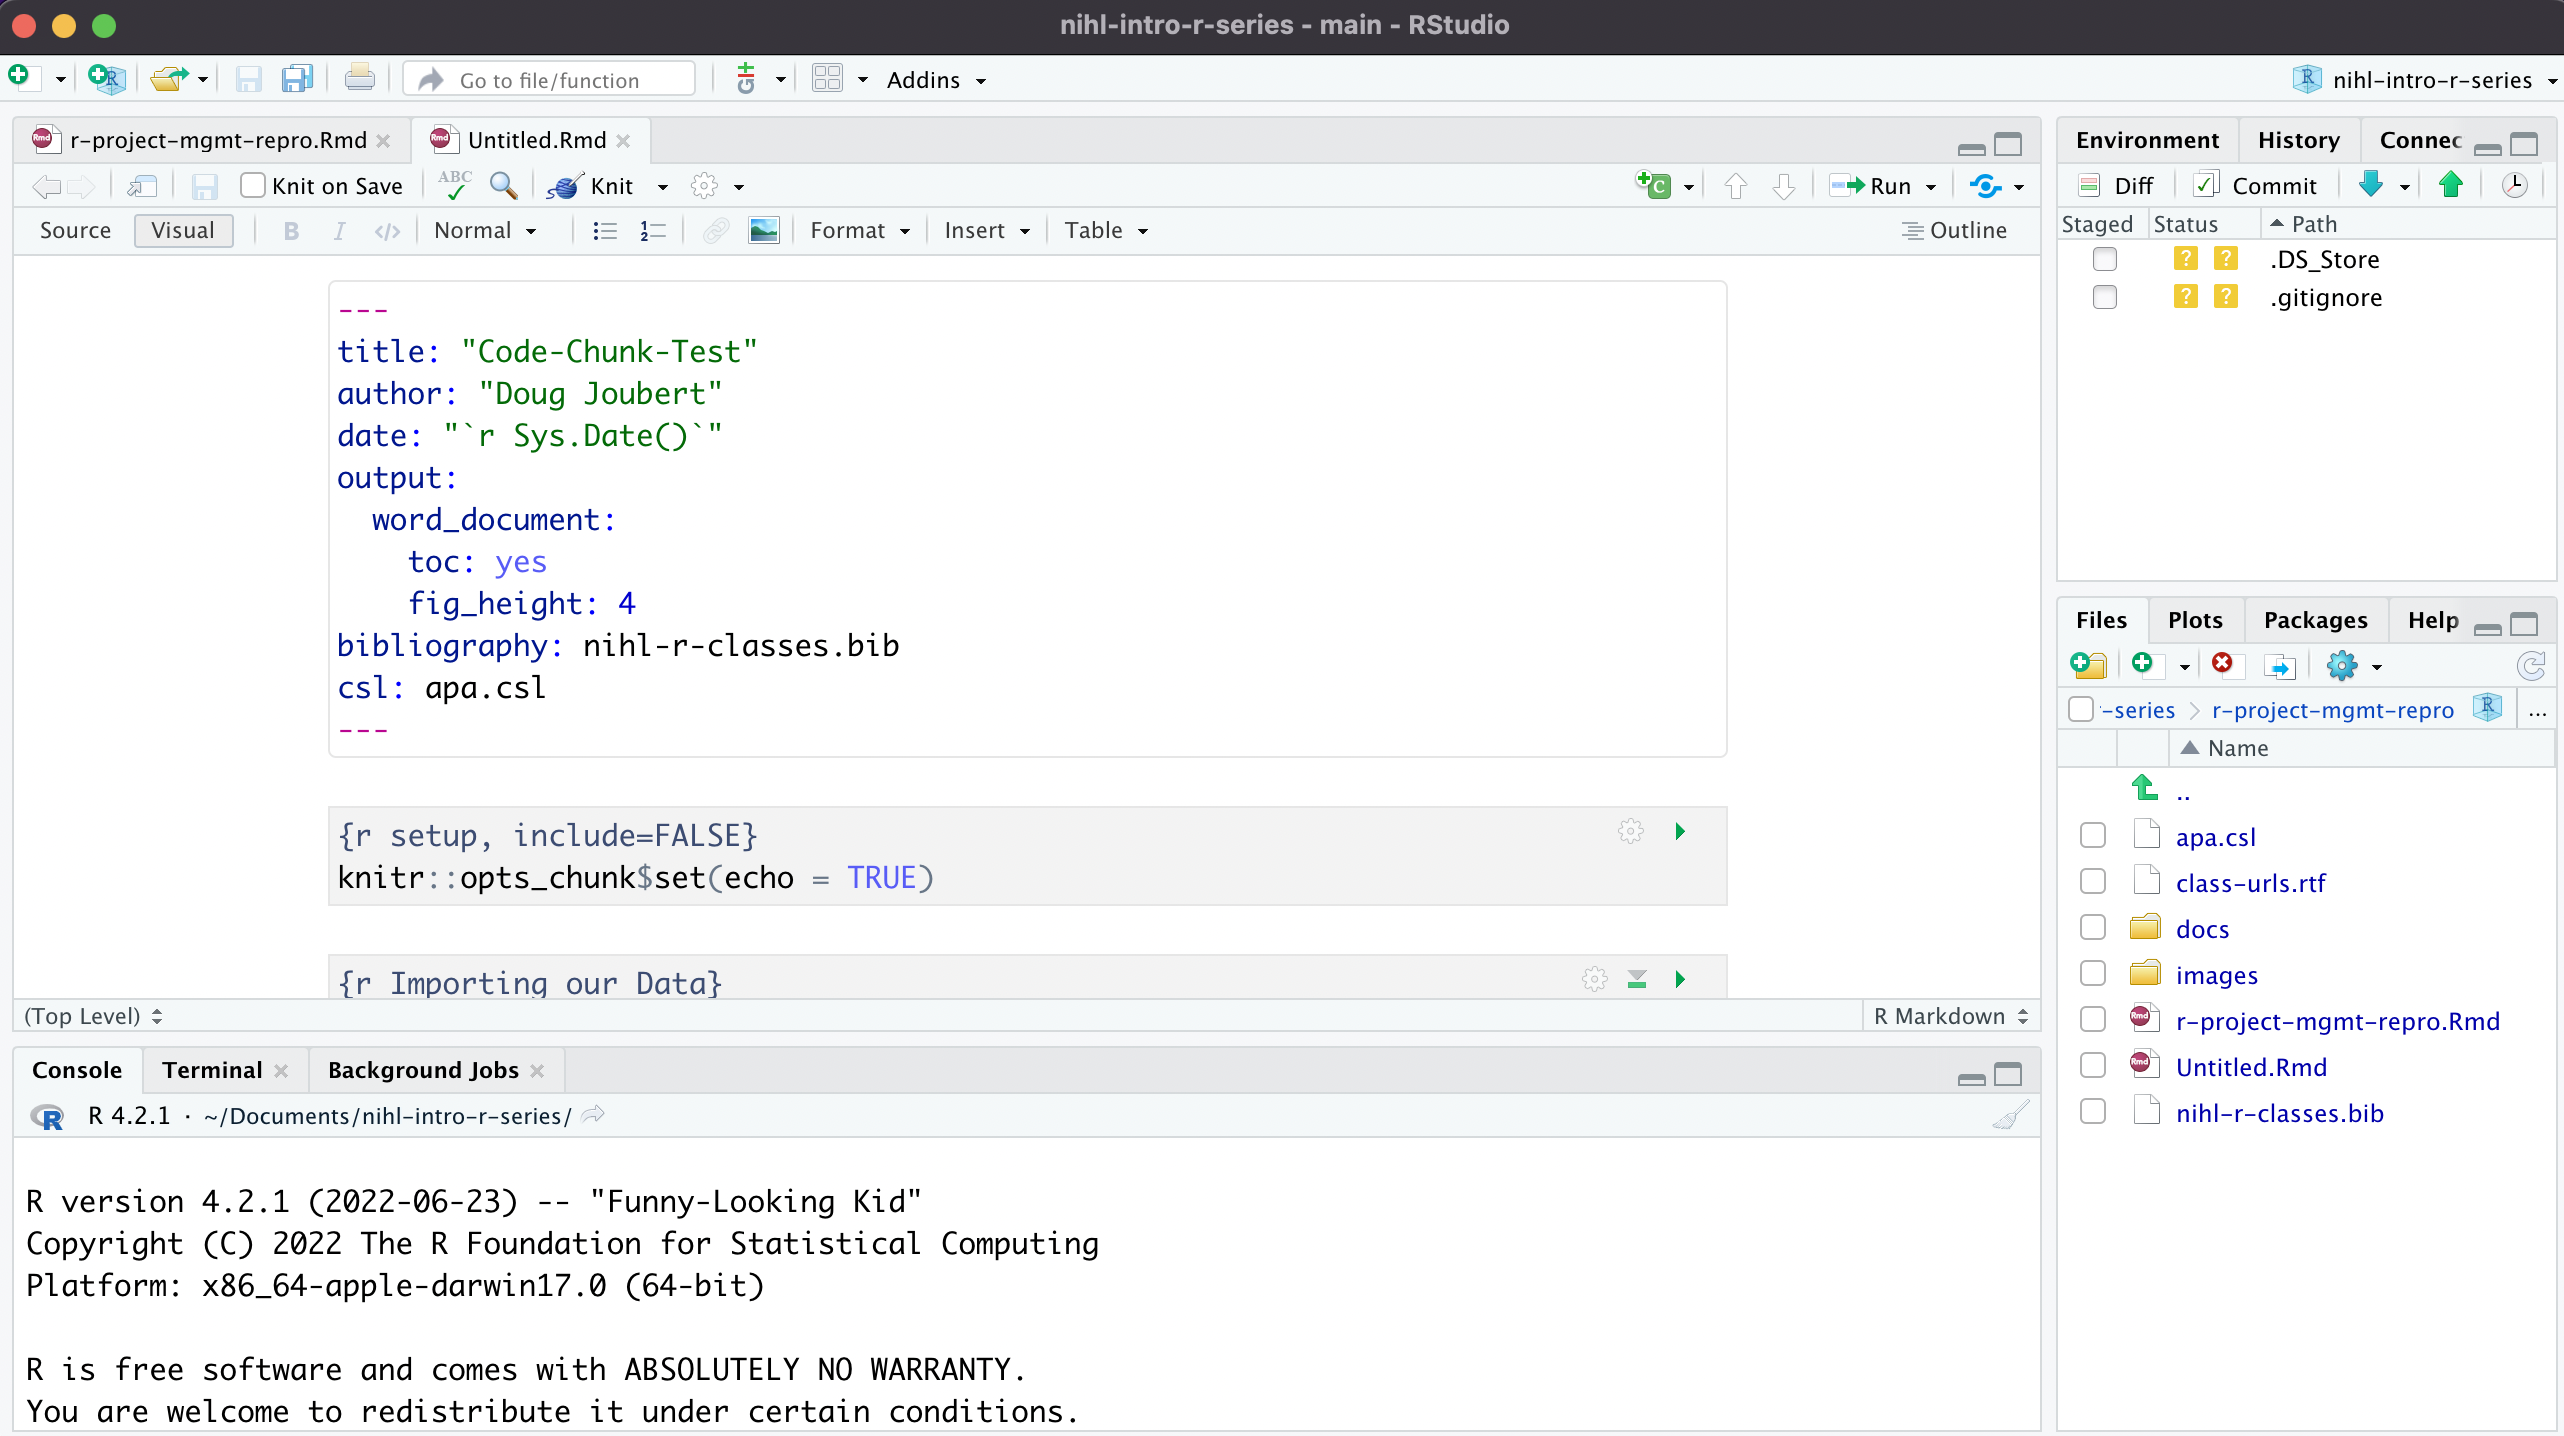
\includegraphics[width=6.6875in,height=\textheight]{images/bib-06.png}

Figure 22: Modifying the RMD header.

Choose Insert\textgreater Citation within RStudio. When you do this, you
should see the records in the linked bib file {[}Figure 23{]}.

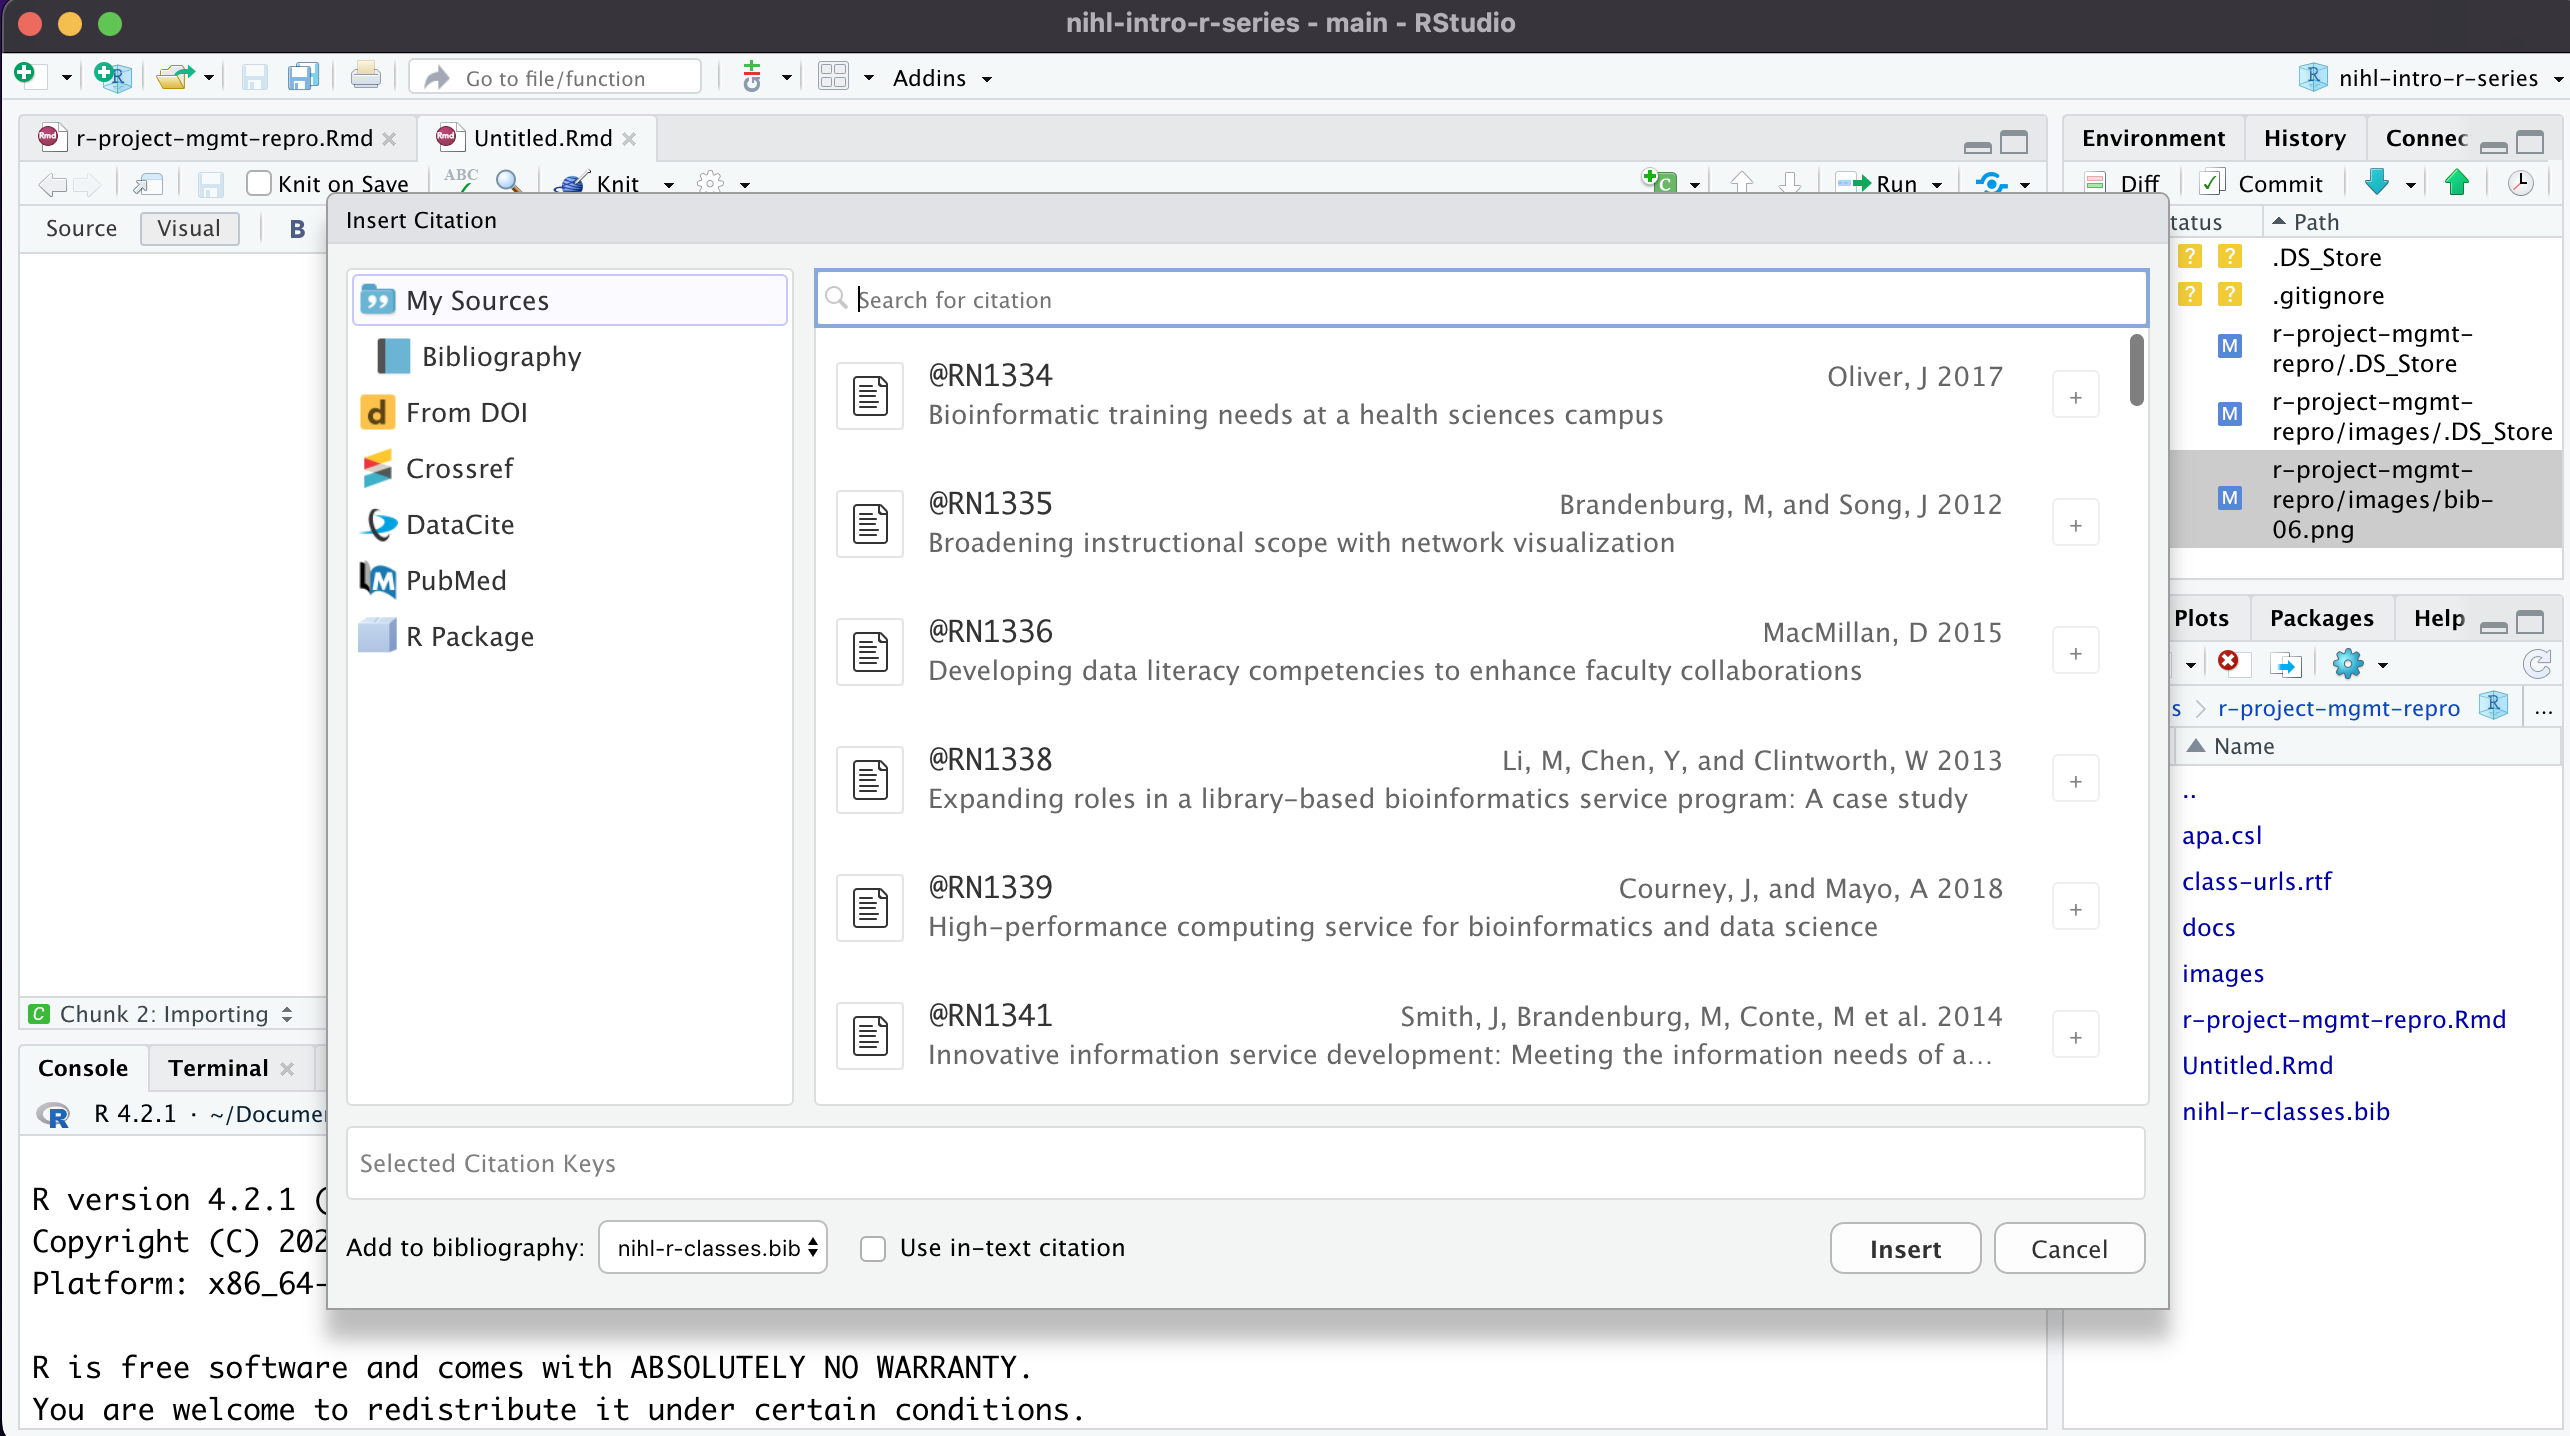
\includegraphics[width=6.66667in,height=\textheight]{images/bib-07.png}

Figure 23: Inserting a citation in RStudio in Visual Mode.

The search box in Figure 23 is a free text search. This means that it
will search on the Author names and the title. Thus, if I search for the
name \textbf{Cimino}, the reference list will filter to contain records
that match my search string {[}Figure 24.

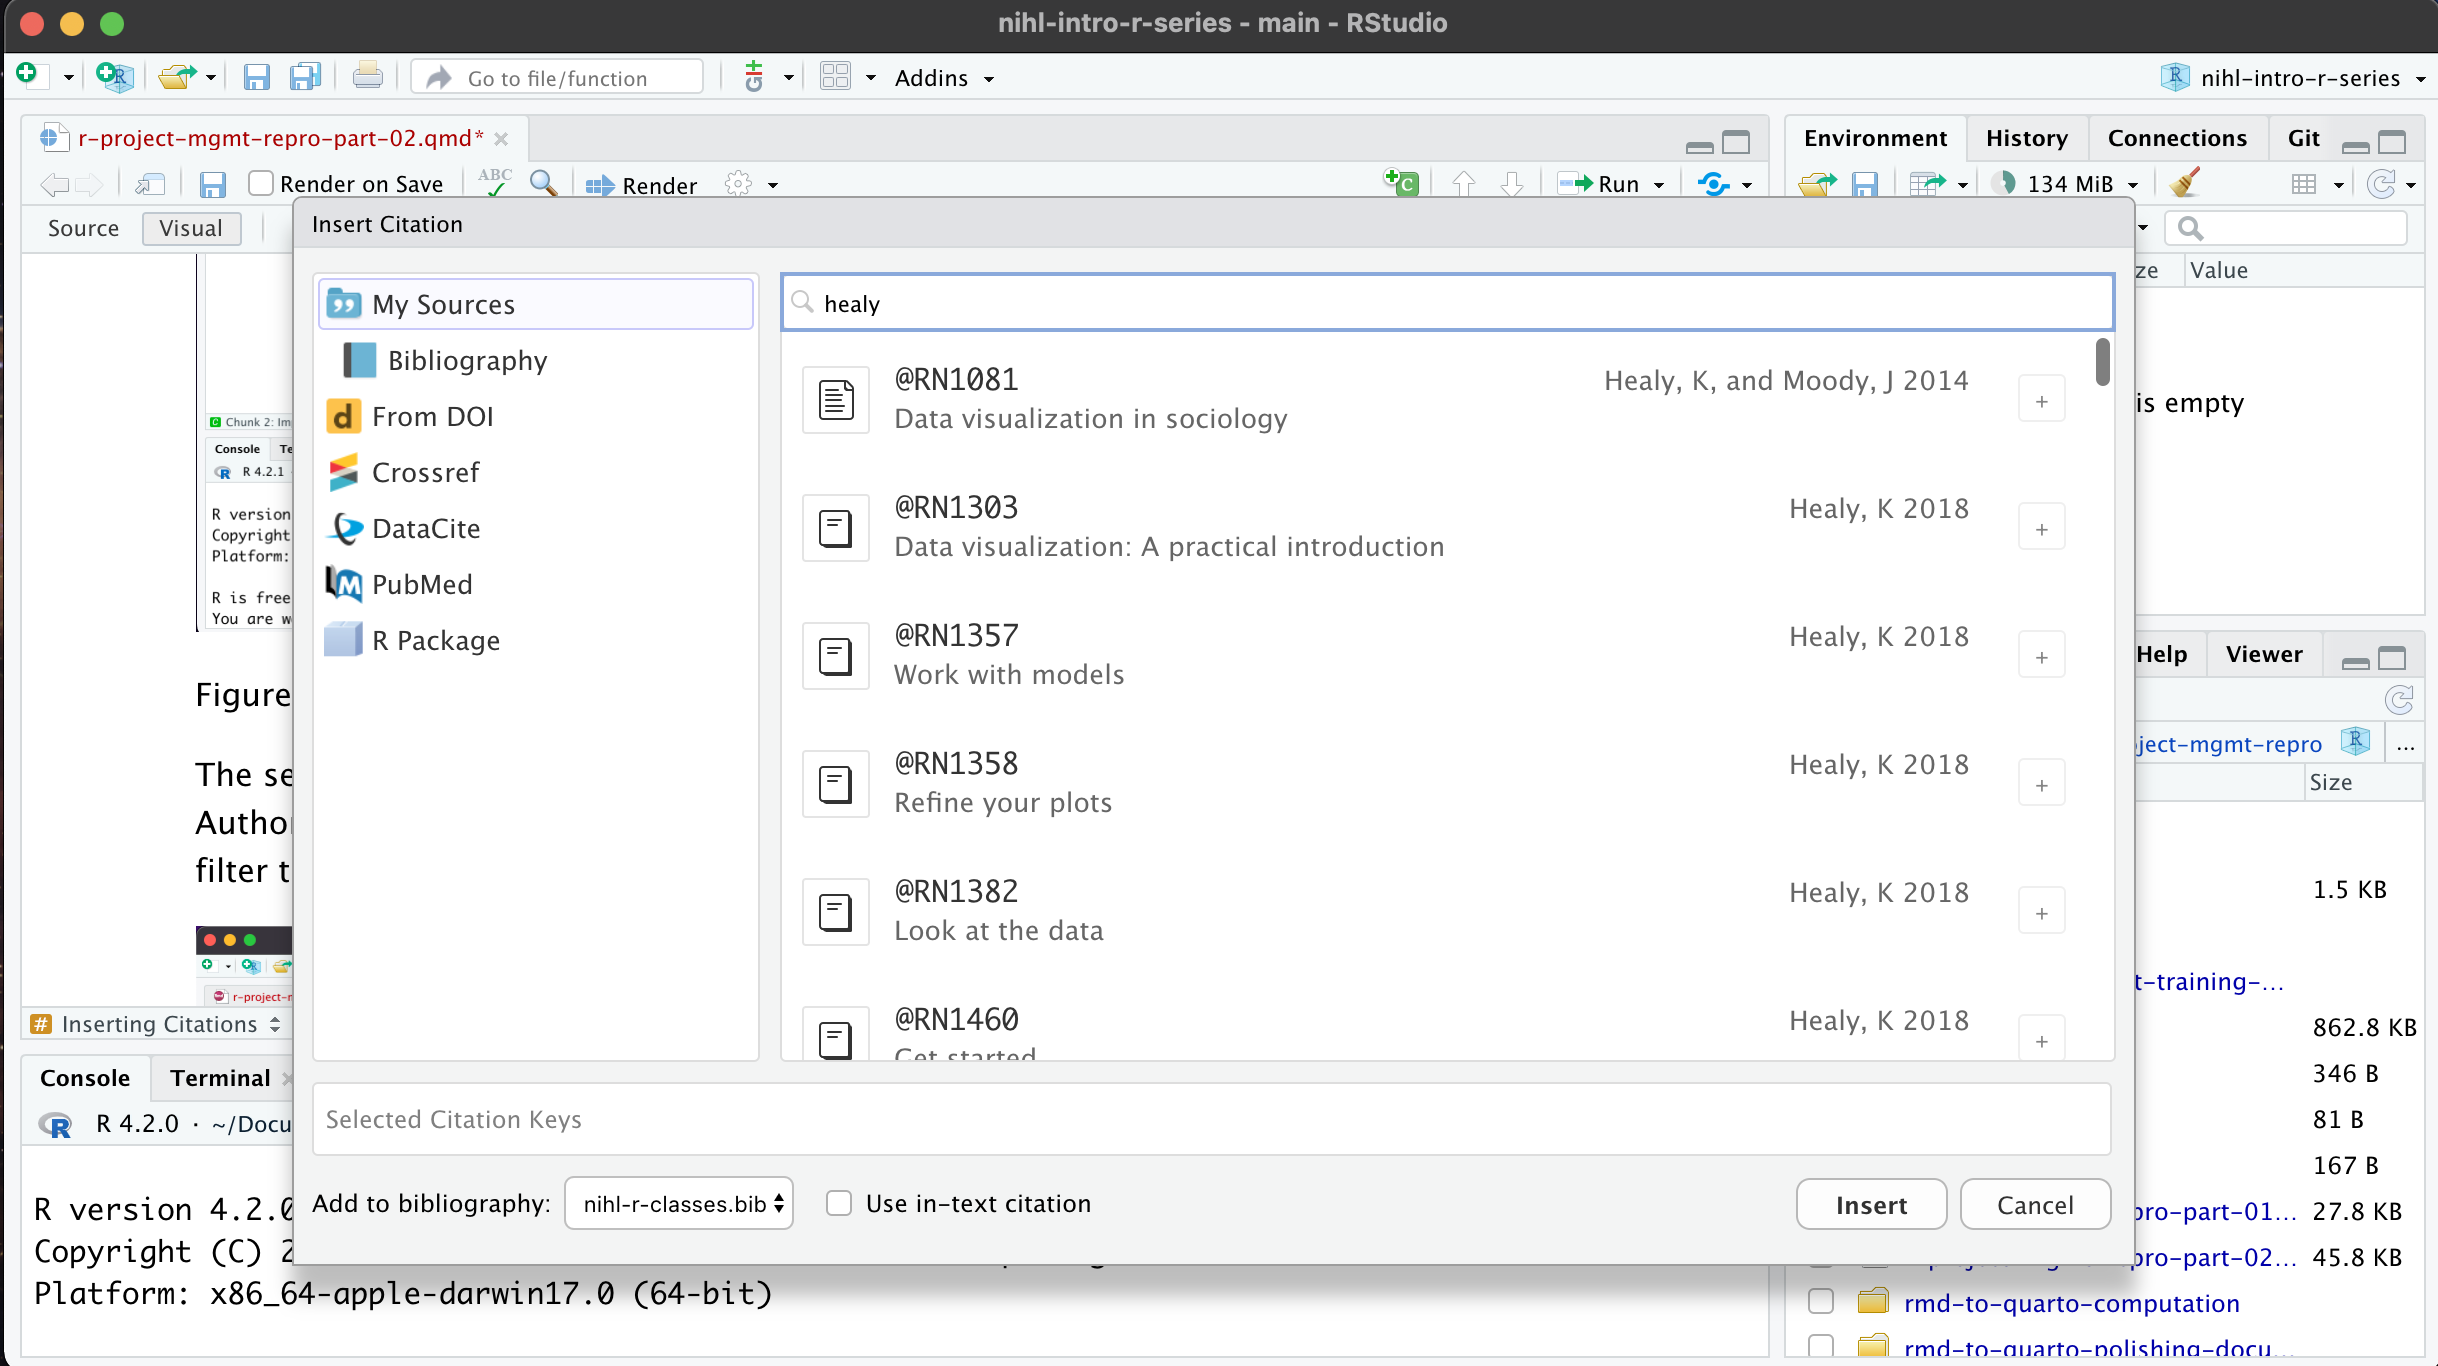
\includegraphics[width=6.66667in,height=\textheight]{images/bib-08.png}

Figure 24: Searching for a record in your bib file.

The record number should appear at the insertion point in your RMD file
{[}Figure 25{]}.

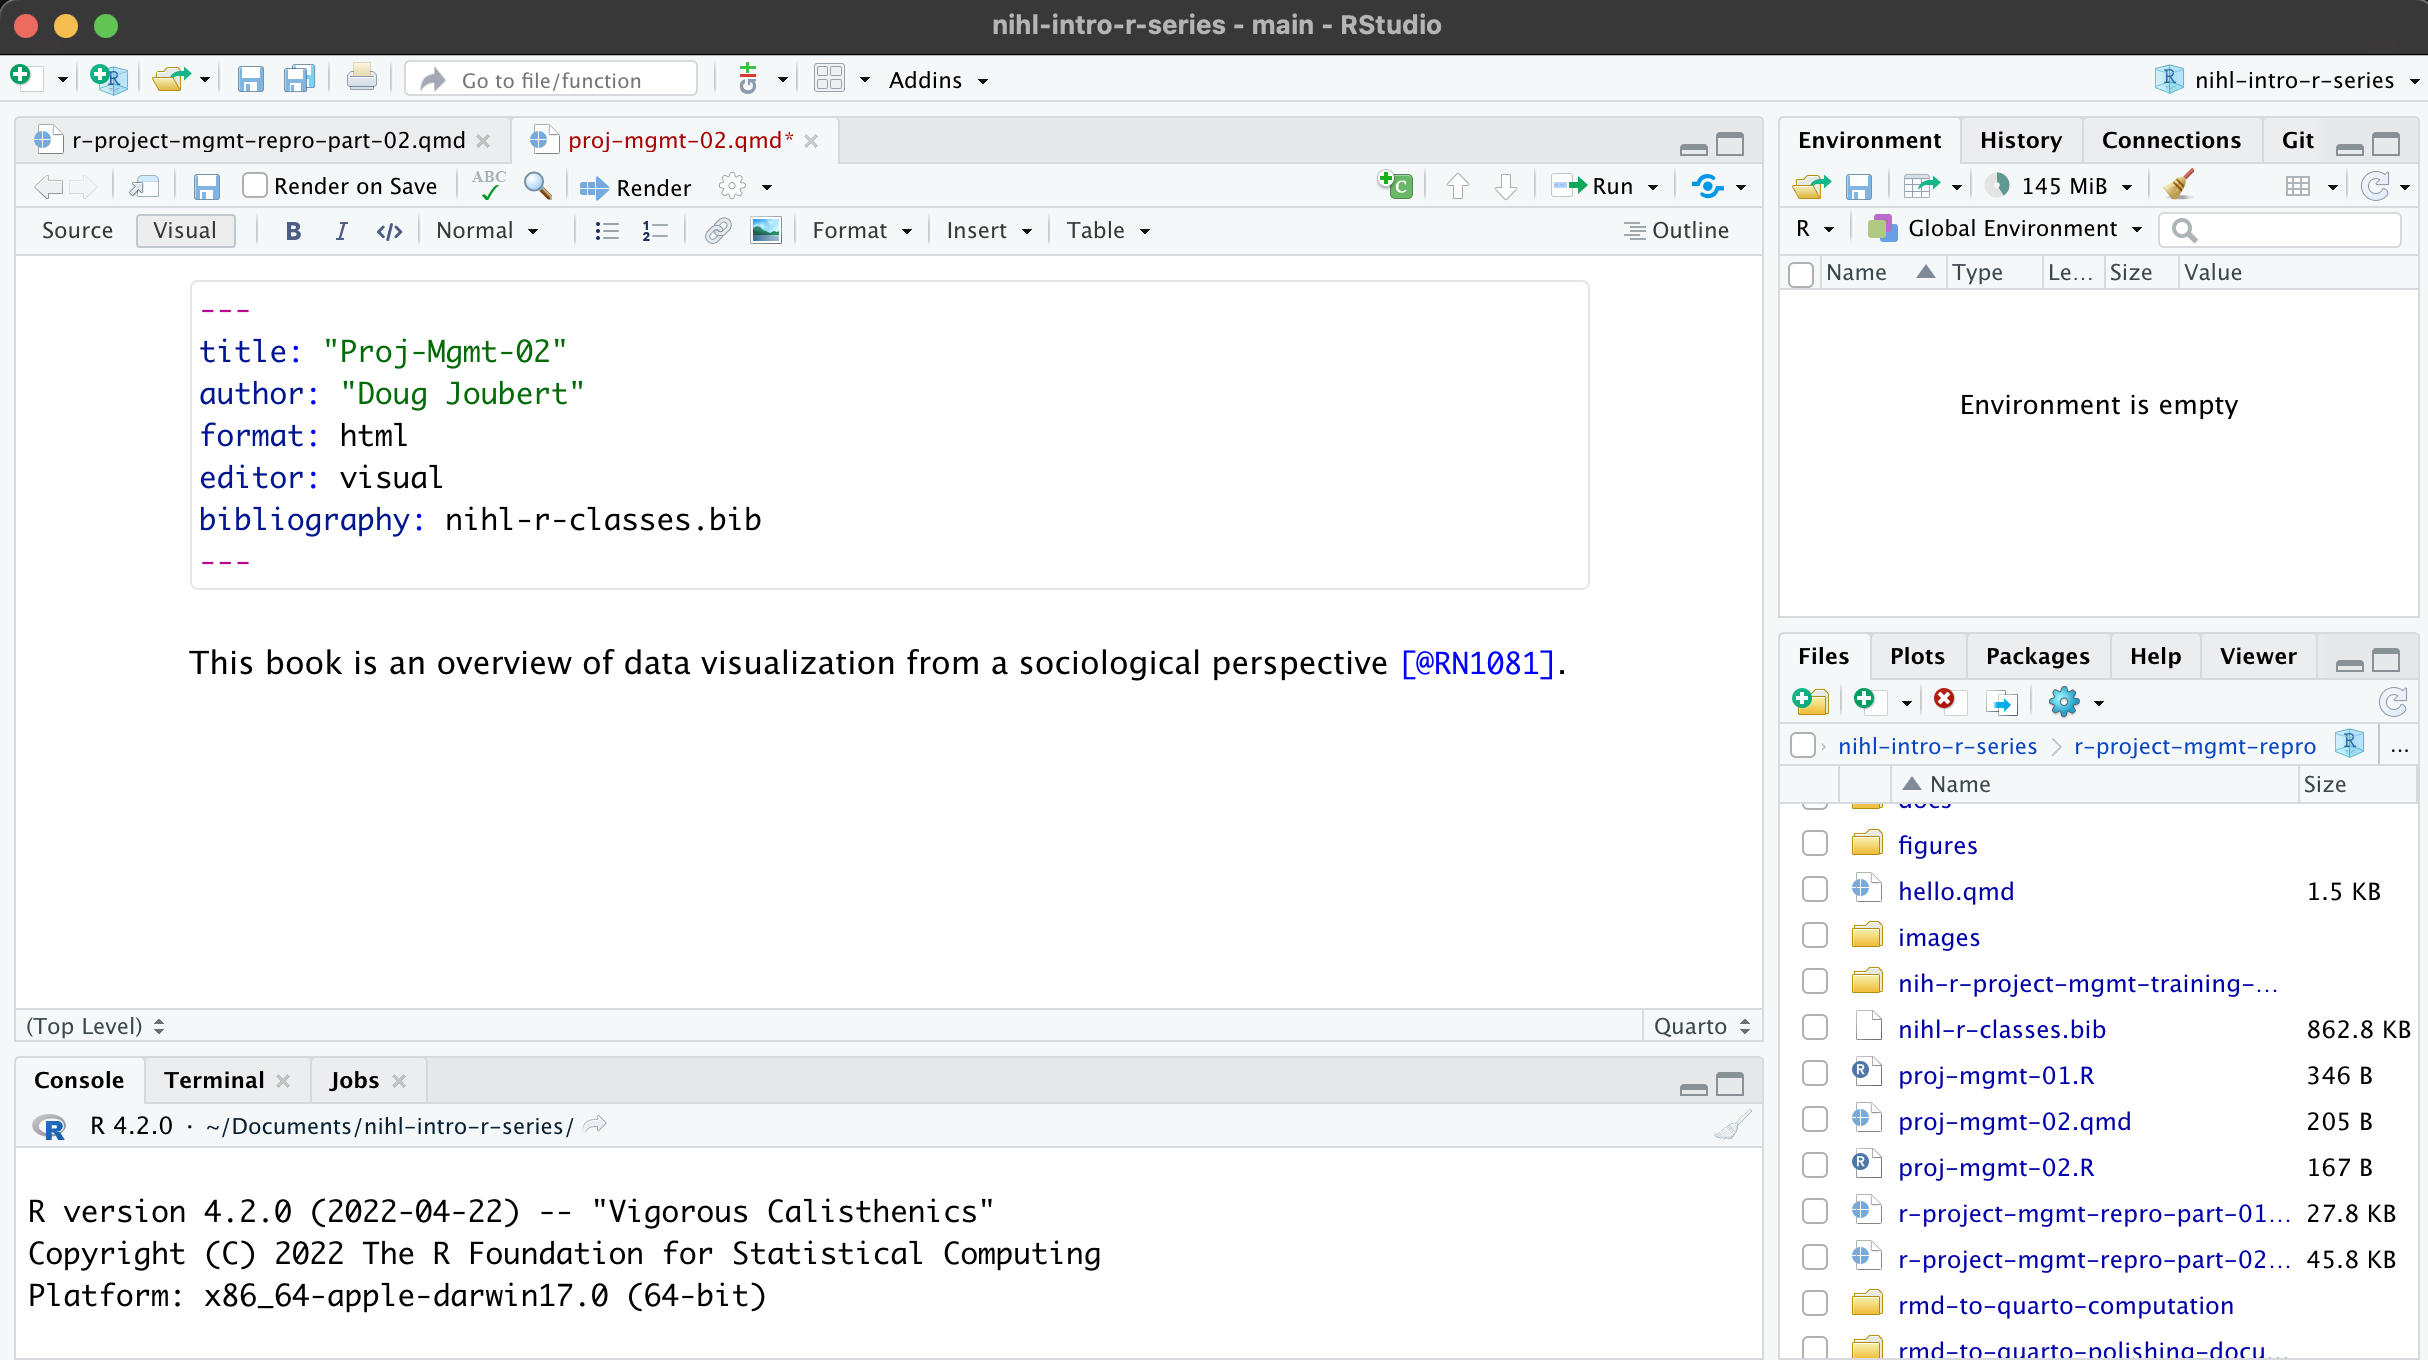
\includegraphics[width=6.66667in,height=\textheight]{images/bib-09.png}

Figure 25: Reference inserted into a RMD document.

\hypertarget{changing-citation-styles}{%
\subsection{\texorpdfstring{\textbf{Changing Citation
Styles}}{Changing Citation Styles}}\label{changing-citation-styles}}

By default, RStudio via Pandoc will use a Chicago author-date format for
citations and references. To use another style, you will need to specify
a CSL (Citation Style Language) file in the csl metadata field in the
YAML.

You can find CSL formats on the
\href{https://www.zotero.org/styles}{Zotero Style Repository}, which
makes it easy to search for and download your desired style.

Download the format you wish to use and call it out in the YAML. I have
already saved the APA CSL file in the project folder. But if you would
like to follow the process or try another style, go to the Zotero Style
repo and select \href{https://www.zotero.org/styles/apa}{American
Psychological Association 7th edition} or any other style of your
choice. You will notice that it will automatically download the file
(e.g.~\texttt{apa.csl}). Make sure to save it to your project directory
in report/source folder. In the YAML we have to call the exact name of
the file preceded by ``csl:'' The Header of your RMD file should now
look like this {[}Figure 26{]}:

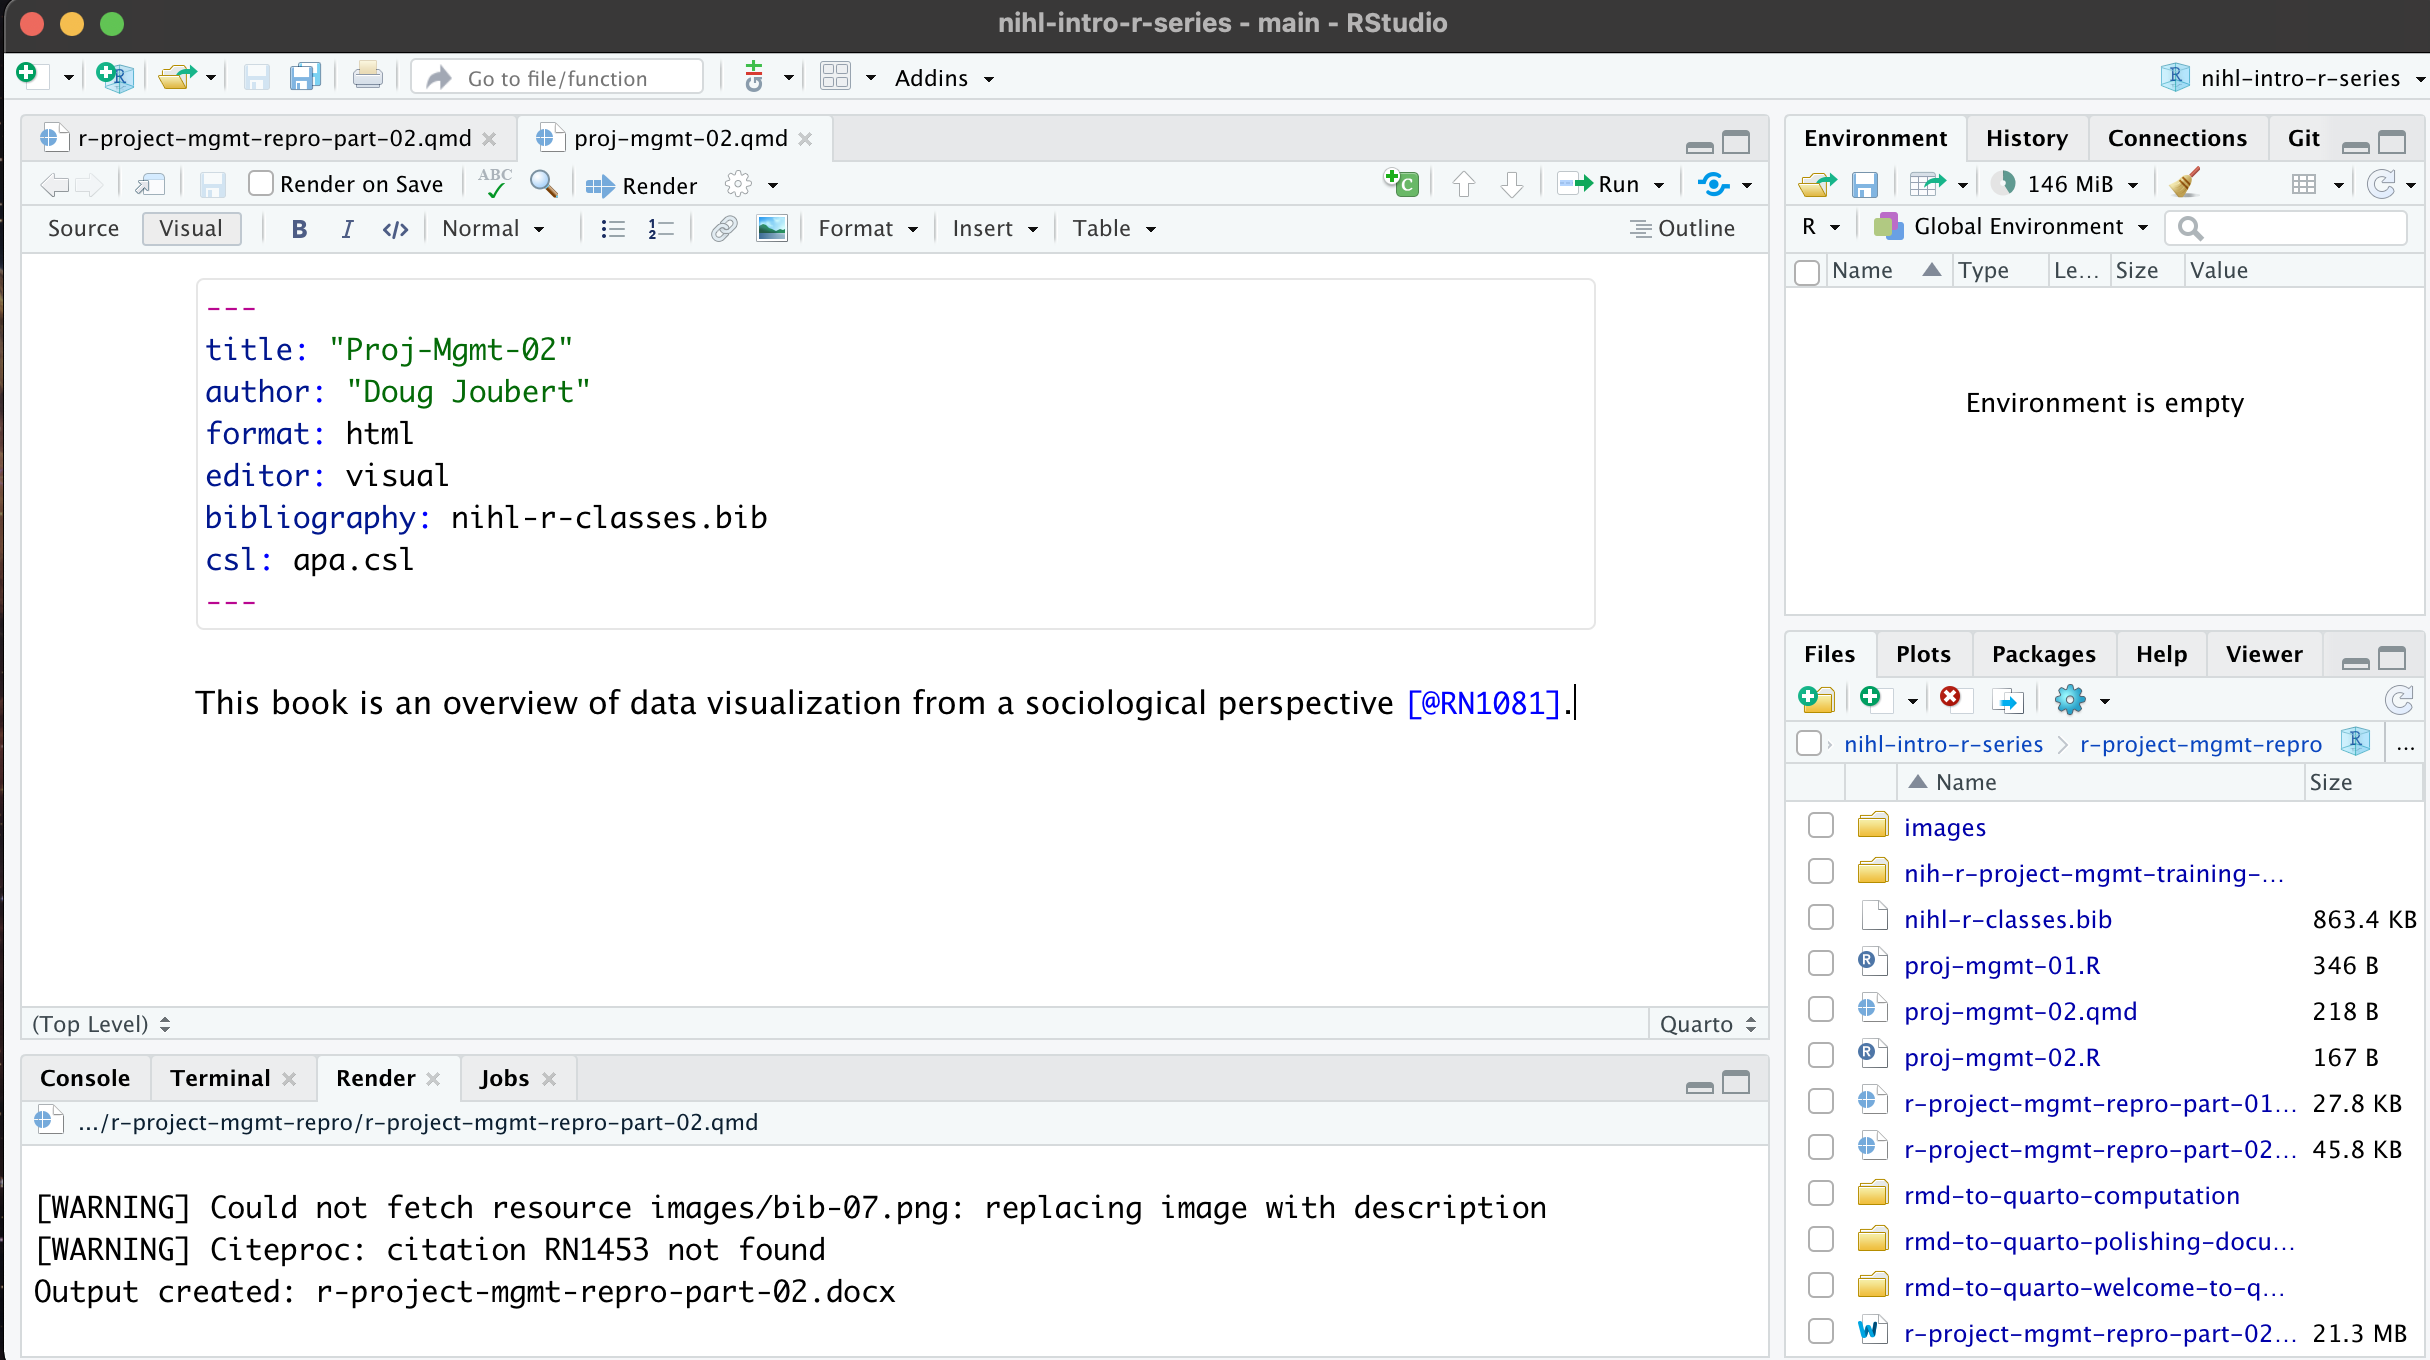
\includegraphics[width=6.66667in,height=\textheight]{images/bib-10.png}

Figure 26: RMD Header with a linked bib file and output style.

The bibliography will be formatted when you Knit your RMD file {[}Figure
27{]}. In Figure 27 I have knitted the RMD document in html format.

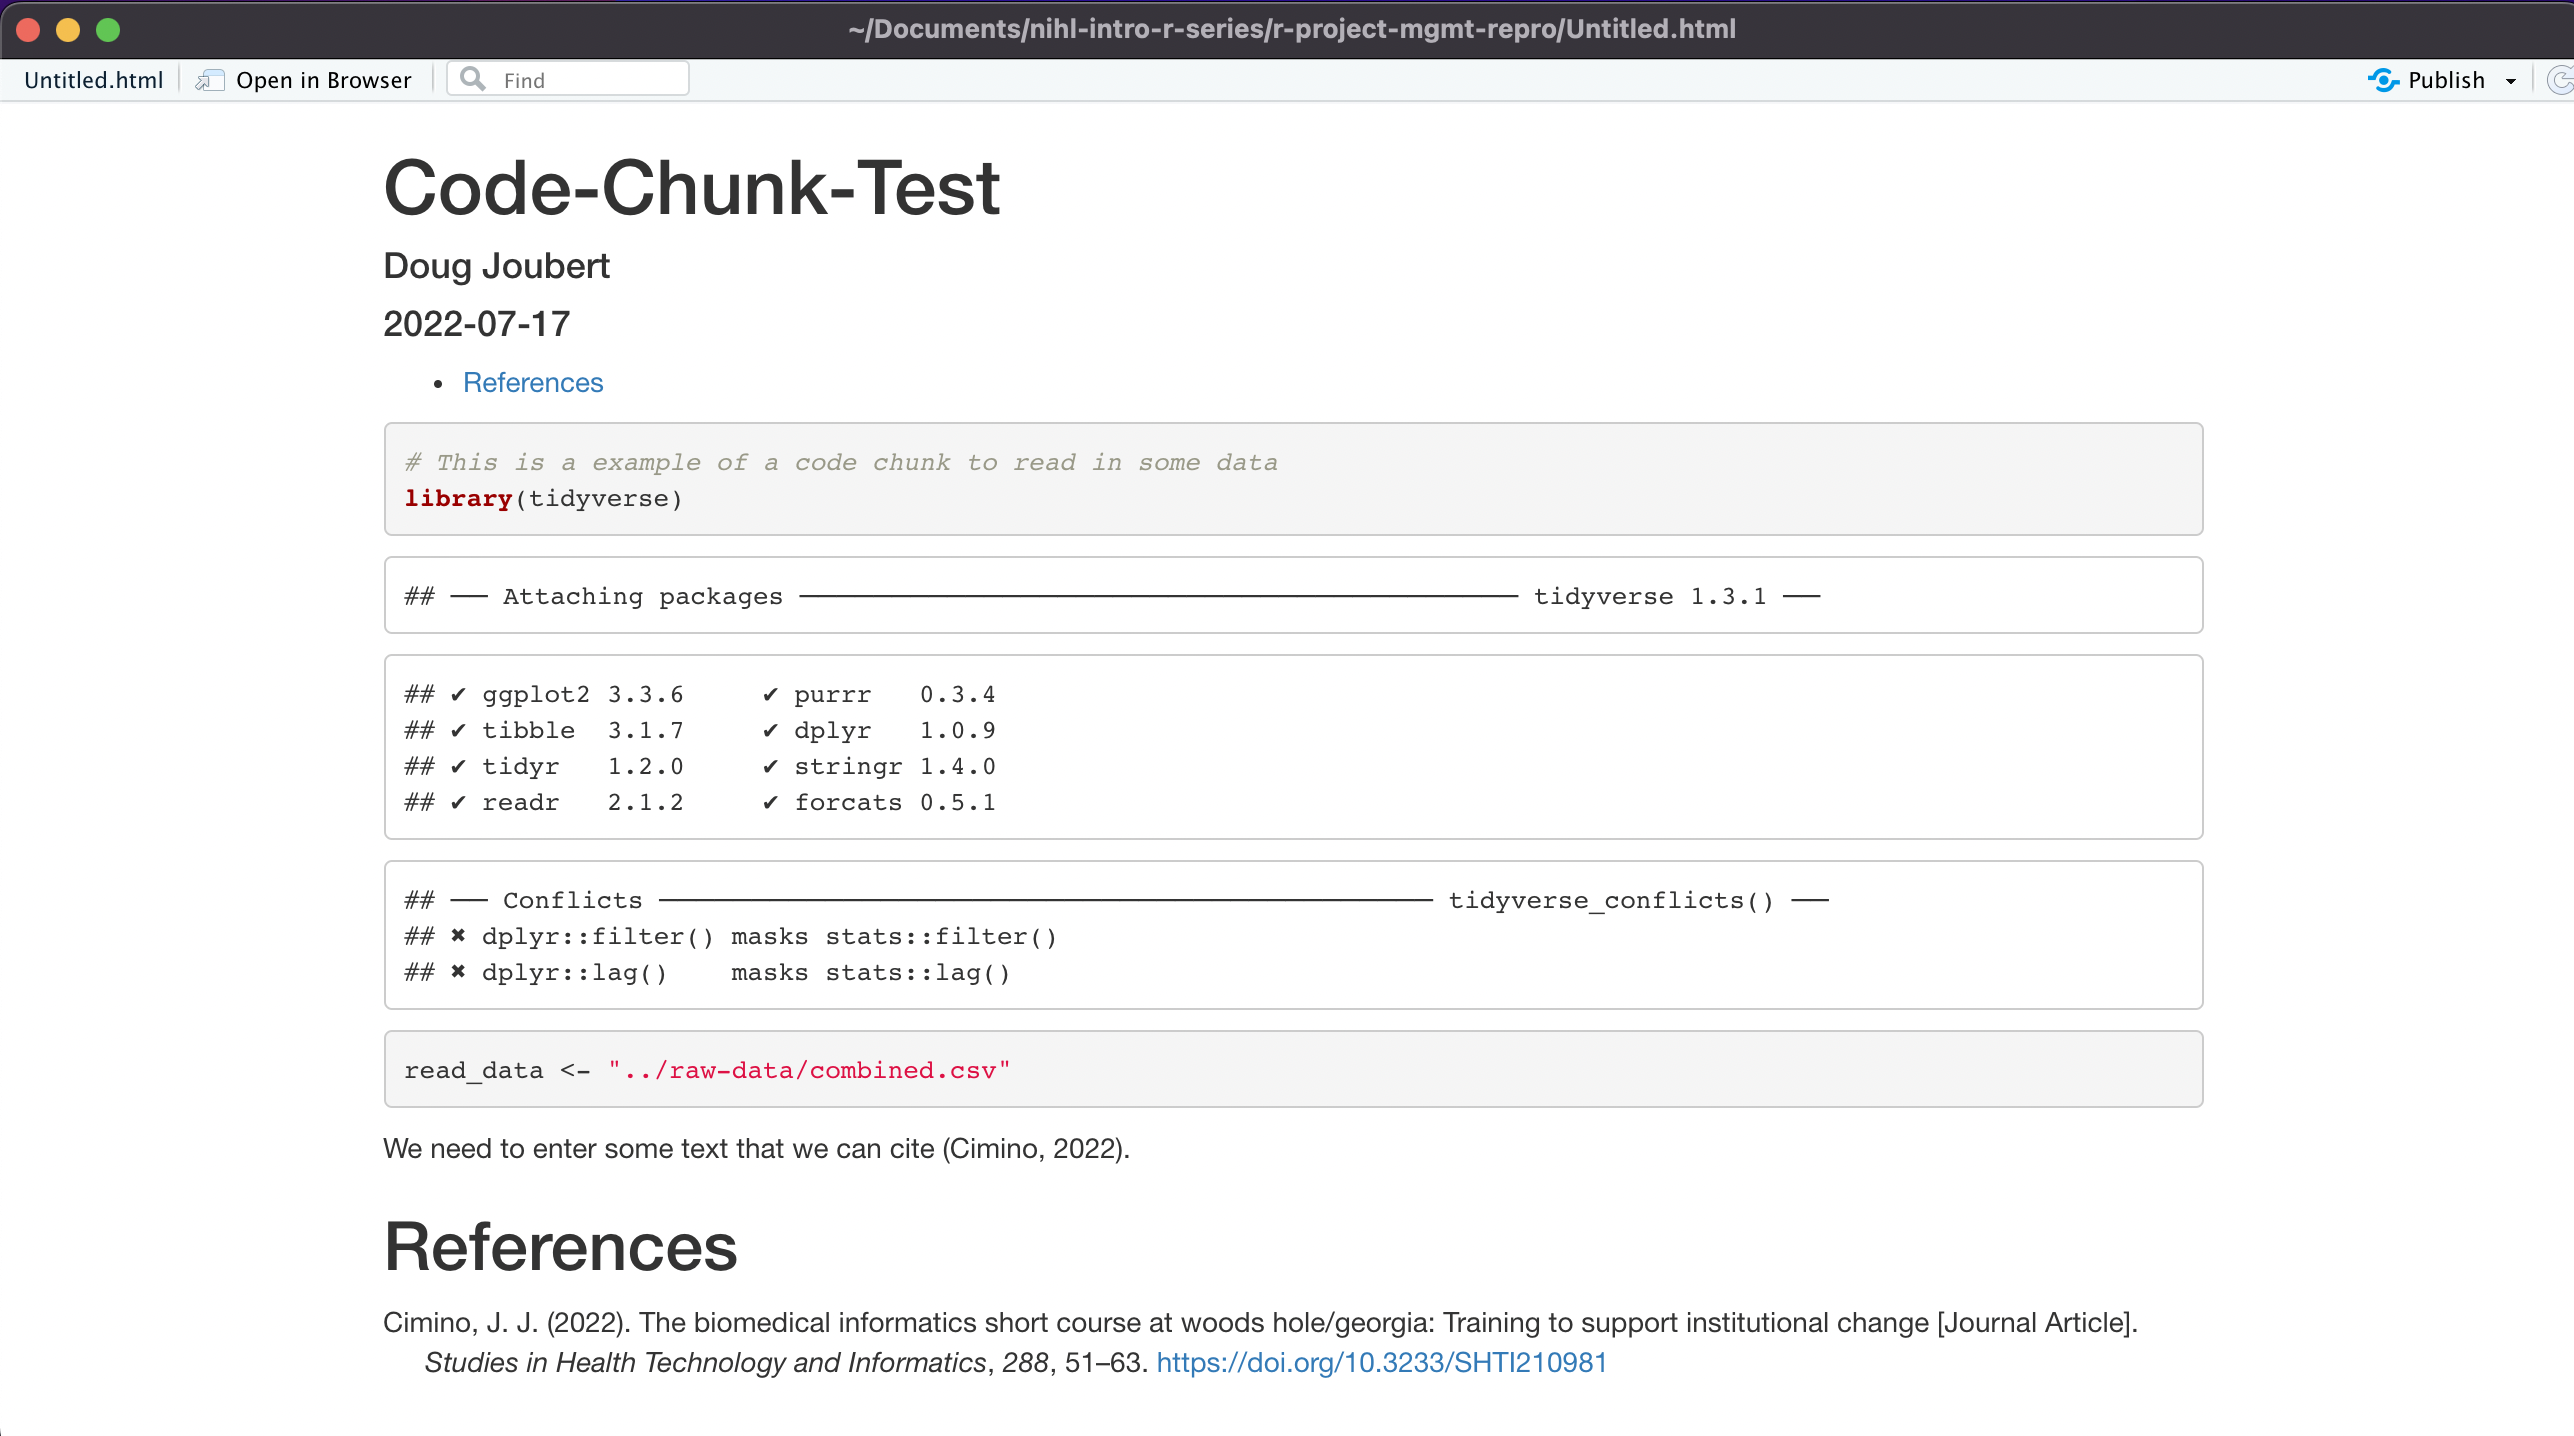
\includegraphics[width=6.66667in,height=\textheight]{images/bib-11.png}

Figure 27: Knitted document with formatted bibliography.

\hypertarget{publishing-your-project}{%
\section{Publishing your project}\label{publishing-your-project}}

\hypertarget{licenses}{%
\section{Licenses}\label{licenses}}

Licensed under \href{https://creativecommons.org/licenses/by/4.0/}{CC-BY
4.0} 2022 by
\href{https://carpentries-incubator.github.io/Reproducible-Publications-with-RStudio/CITATION}{the
authors}.

\hypertarget{references}{%
\section*{References}\label{references}}
\addcontentsline{toc}{section}{References}

\hypertarget{refs}{}
\begin{CSLReferences}{1}{0}
\leavevmode\vadjust pre{\hypertarget{ref-RN1683}{}}%
Baker, M. (2016). 1,500 scientists lift the lid on reproducibility
{[}Journal Article{]}. \emph{Nature}, \emph{533}(7604), 452--454.
\url{https://doi.org/10.1038/533452a}

\end{CSLReferences}

\end{document}
